\chapter{Dataset and Event Reconstruction}\label{ch:dataset-reconstruction}
\begin{figure}[htbp]
	\centering
	\hfill
	\subfloat[] {\label{fig:reco-luminosity-runI}
		\resizebox{0.4\textwidth}{!}{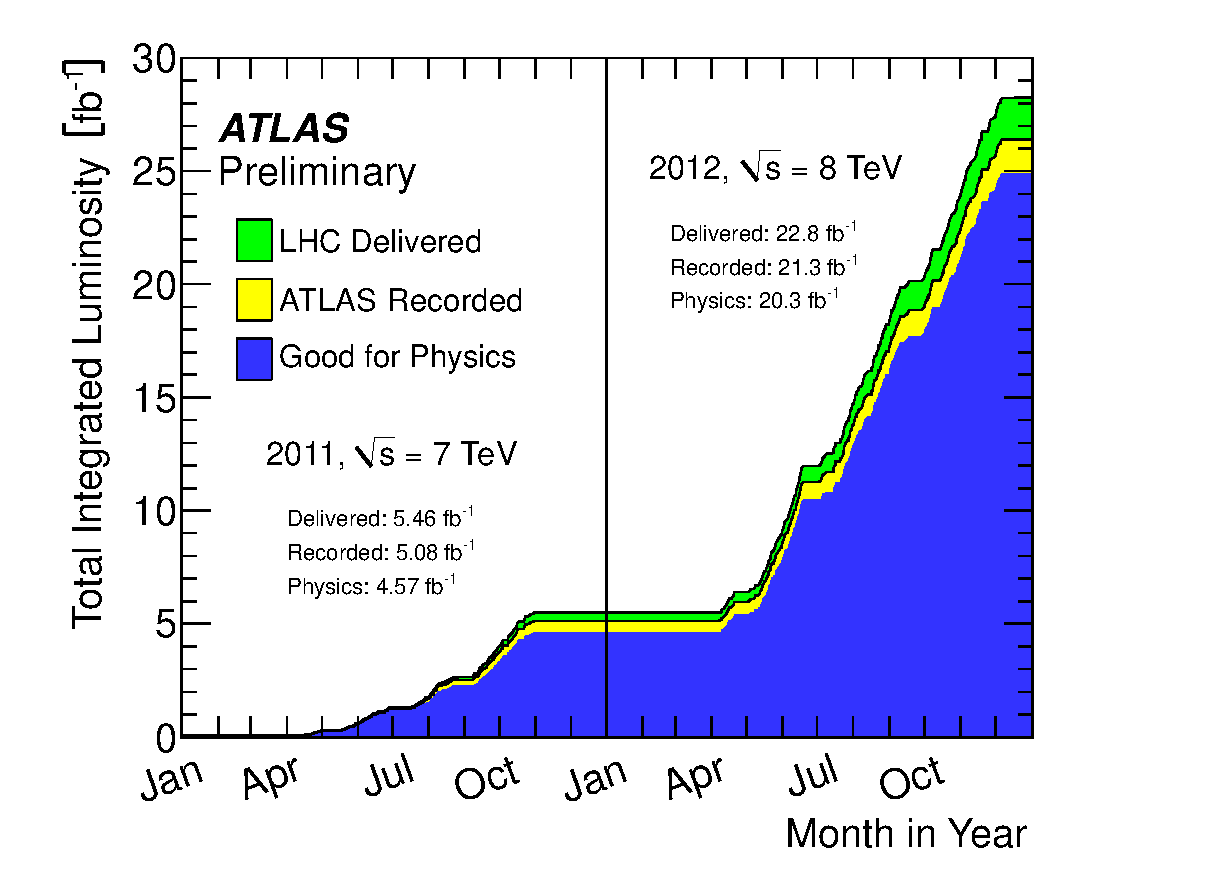
\includegraphics{figures/ch4-reconstruction/intlumivstime2011-2012DQ.eps}}
	}
	\hfill
	\subfloat[] {\label{fig:reco-luminosity-pileup}
		\resizebox{0.4\textwidth}{!}{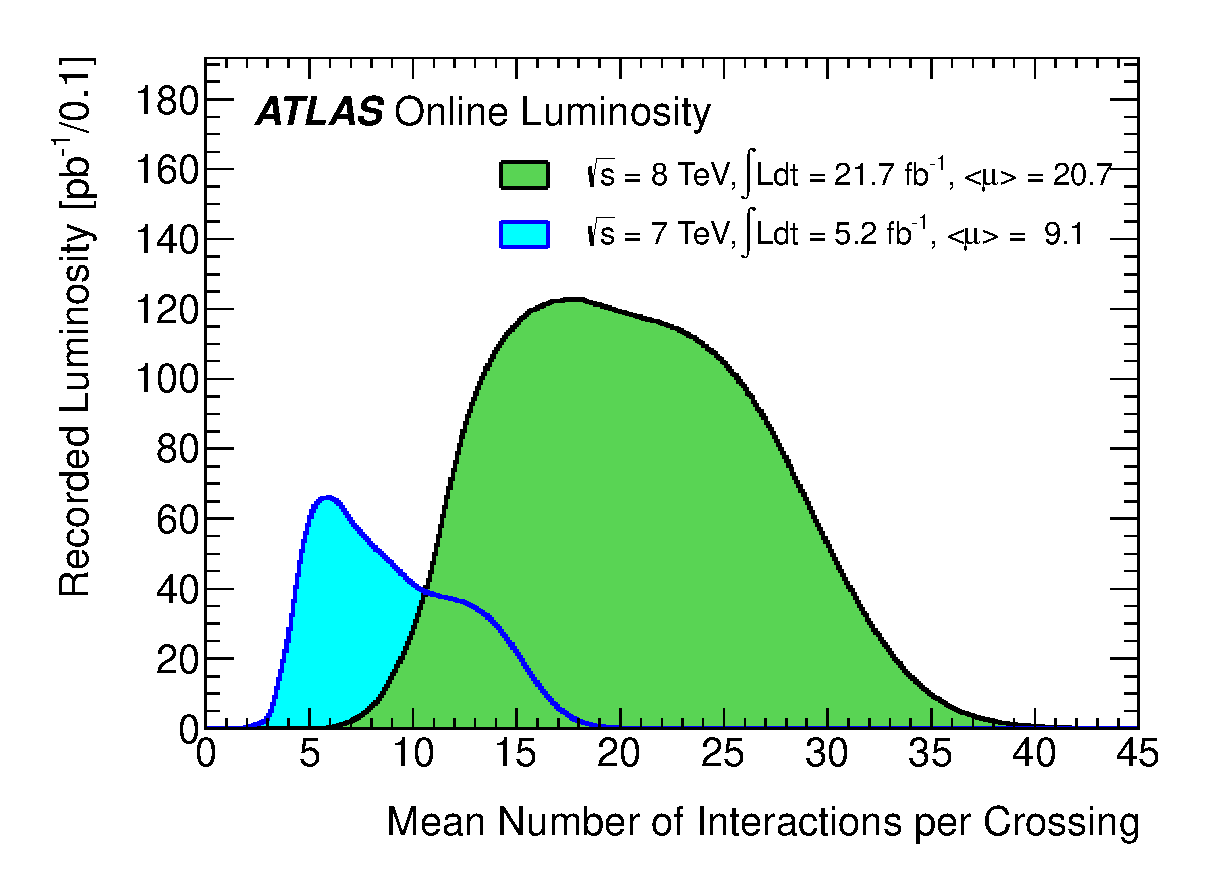
\includegraphics{figures/ch4-reconstruction/mu_2011_2012-dec.eps}}
	}
	\hfill
	\caption{Left: The cumulative delivered, recorded, and physics-ready integrated luminosity versus time in 2011-2011. Right: Distribution of the number of interactions per bunch crossing in events recorded in 2011-2012.}
	
\end{figure}

The ATLAS Run I data were recorded from 2011 to 2012, with a center-of-mass collision energy of $\sqrt{s}=7 \TeV$ in 2011 and $\sqrt{s}=8 \TeV$ during 2012. Integrated luminosities of $\int L dt=5.46 \ifb$, and $22.8 \ifb$ were delivered by the LHC in the two years, of which $5.08 \ifb$ and $21.3 \ifb$ were recorded by the ATLAS detector. The recorded luminosity accounts for the DAQ inefficiency, as well as the \emph{warm start} period after the declaration of stable beams, during which the tracking detectors are ramped to high voltage and the pixel detector preamplifiers are turned on. After masking data recorded while one or more detector subsystems were not functioning properly, $4.57 \ifb$ and $20.3 \ifb$ of data are considered ready for physics analyses. The volume of delivered, recorded, and physics-ready data are shown as a function of time in figure~\ref{fig:reco-luminosity-runI}. 

During Run I, the LHC was operated with a bunch spacing of $50 \ns$. The increases in the data-taking rate generally correspond to an increase in the number of simultaneous $pp$ interactions per bunch crossing, or \emph{pileup}, denoted $\mu$. The distribution of pileup values for 2011 and 2012 data are shown in figure~\ref{fig:reco-luminosity-pileup}. 


\section{Luminosity Measurement}\label{sec:luminosity-measurement}
The instantaneous luminosity at a $pp$ collider is given by:

\begin{equation}
	\mathcal{L} = \frac{R_{\mathrm{inel}}}{\sigma_{\mathrm{inel}}},
\end{equation}

where $R_{\mathrm{inel}}$ is the rate of inelastic $pp$ collisions, and $\sigma_{\mathrm{inel}}$ is the $pp$ inelastic cross section. For a storage ring with a revolution frequency $f_r$ and $n_b$ colliding bunch pairs, the instantaneous luminosity can be written in terms of the average number of inelastic $pp$ collisions per bunch cross, $\mu$, as 

\begin{equation}
	\mathcal{L} = \frac{\mu f_r n_b}{\sigma_{\mathrm{inel}}}.
\end{equation}

The instantaneous luminosity is measured by ATLAS using several detectors and algorithms, which have some efficiency $\epsilon$ to detect a $pp$ interaction, and measure the \emph{visible} number of interactions per bunch crossing, $\mu_{\mathrm{vis}} = \epsilon \mu$. Defining the visible cross section to be $\sigma_{\mathrm{vis}}\equiv \epsilon \sigma_{\mathrm{vis}}$, the instantaneous luminosity as measured by a particular detector is:

\begin{equation}\label{eqn:reco-luminosity-detected}
	\mathcal{L} = \frac{\mu_{\mathrm{vis}} f_r n_b}{\sigma_{\mathrm{vis}}}.
\end{equation}

The visible cross section is a calibration constant for a particular detector, which is determined during dedicated calibration runs in which the luminosity is determined directly from the geometry of the beams. The calibration procedure is described in section~\ref{sec:reco-luminosity-calibration}. 

\subsection{Luminosity Detectors}\label{sec:reco-luminosity-detectors}
ATLAS performs many redundant luminosity measurements using several detectors. The detectors fall into two categories. \emph{Event counting} detectors have a binary response, returning a 0 or 1 depending on whether a bunch crossing satisfies a set of criteria defined to detect an inelastic $pp$ collision. Such detectors essentially measure $p(0;\,\mu)$, the probability that an event falls in the first bin of a Poisson distribution, from which the mean $\mu$ be calculated. \emph{Hit counting} detectors, on the other hand, count some quantity proportional to the number of interactions in a given bunch crossing, such as the number of particles identified by a particular detector subsystem. A hit counting measurement typically yields more information about an event at the cost of additional systematic uncertainties.

Ideally, a luminosity detector exhibits the following features: 

\begin{itemize}
	\item The efficiency of the detector should be insensitive to pileup. The visible cross sections are typically measured at $\mu\approx \mathcal{O}(1)$, while a typical data-taking run has $10\lesssim\mu\lesssim50$; it is essential that the visible cross section be constant across this range of pileup values.
	\item The efficiency of the detector should also be constant over long timescales.
	\item The response of the detector and the readout should be very fast. As the LHC bunches are not identical, with different numbers of protons and emittances, it is useful to measure luminosity for each colliding bunch pair, as often as once every $25 \ns$. The colliding bunch pairs are labeled by the bunch crossing identification number, or BCID; consecutive BCIDs are separated by $25 \ns$. 
	\item The efficiency should be high enough to yield sufficient statistics. The data are used in increments as shorts at $20~$s, so the statistics collected over this time scale scale should be high enough that the total uncertainty is dominated by systematic effects. On the other hand, for event counting detectors, the efficiency should not be so high that the detector is saturated. The determination of the mean of a Poisson distribution from the first two bins requires that the first two bins both have adequate statistics. 
	\item The backgrounds should be low and understandable. Detectors can be sensitive to a wide range of phenomena aside from $pp$ collisions, which should not be counted as luminosity. For example, some detectors observe a phenomenon called afterglow, characterized by a small amount of activity in the BCIDs immediately following a collision and likely due to photons from nuclear de-excitations in the detector material. The background can be estimated using the observation that the level of afterglow background is proportional to the luminosity in the colliding BCIDs, and decays away with several time constants. Collisions between a beam and residual gas in the beam pipe, called beam-gas interactions, can also contribute a low level of background, and can be estimated by observing non-colliding bunches passing through the interaction region.
\end{itemize}

The central value of the luminosity measurement is determined by the \emph{beam conditions monitor} (BCM), which fulfills most of these desired criteria. The BCM consists of eight diamond-based particle detectors, four on each side of the interaction point at $|z|=184 \cm$ and $|\eta|=4.2$. The detectors are have a physical cross section of approximately $1 \cm^2$, and are arranged in a cross pattern, with two readouts corresponding to the vertical and horizontal pairs. The design goal of the BCM is to monitor backgrounds and to trigger a beam dump if beam losses towards the inner detector become too high; accordingly, the detector has a very fast readout, and can provide a bunch-by-bunch luminosity measurement with a time resolution of $\sim 0.7 \ns$. The luminosity is measured using event counting, and can be measured using any combination of the readouts. The configurations used require hits in either the vertical pair (BCMV) or the horizontal pair (BCMH), and either coincident hits on both sides of the interaction point (AND) or a single hit on either side (OR). The small size of the readouts leads to an efficiency of approximately 7\% in the OR configuration, which allows for sufficient statistics without saturating the detector. 

The LUCID detector provides a supplementary, bunch-by-bunch, event counting-based luminosity measurement using sixteen Cherenkov detectors surrounding the beampipe on each side of the interaction point at $|z|=17~\mbox{m}$, covering a pseudorapidity range of $5.6<|\eta|<6.0$. The Cherenkov detectors are polished aluminum tubes filled with C$_4$F$_{10}$ gas. The Cherekov photons induced by charged particles traversing the gas are collected by photomultiplier tubes (PMTs) located at the far end of the tubes. Additional Cherenkov photons are produced in the quartz window separating the tube volume from the PMT. In this initial configuration, the typical single-particle yield is 60-70 photoelectrons due to photons created in the gas, and about 40 photoelectrons due to the quartz window. A hit is recorded if the PMT signal exceeds a preset threshold, corresponding to about 15 photoelectrons. However, the higher per-bunch instantaneous luminosities due to the LHC operating with $50 \ns$ spacing rather than the design $25 \ns$ spacing led to saturation of the detectors, and hence on 30 July 2011, the gas was removed from the Cherenkov tubes to reduce the efficiency. The removal of the gas also improved the detector's stability and linearity with respect to pileup. Relative comparisons with other detectors were used to reestablish the detector calibration.

Several detector subsystems nominally designed for physics object reconstruction are also used for hit counting-based luminosity measurements. Algorithms using the tile calorimeter and the forward calorimeters (see section~\ref{sec:ATLAS-calorimeters}) determine the luminosity from detector currents proportional to the total particle flux in small regions of the calorimeters. The tile calorimeter algorithm monitors the PMT currents corresponding to a few selected cells near $|\eta|=1.25$, where the highest sensitivity to changes in the luminosity is observed. Similarly, the forward calorimeter algorithm monitors the currents in the high voltage lines. In both cases, the detector response is too slow to provide a bunch-by-bunch measurement, and the current response is not sensitive to the low instantaneous luminosities during the dedicated calibration runs, requiring the calibration to be set using a relative comparison with LUCID. On the other hand, the detectors exhibit good linearity of response with pileup, and good short-term stability. 

Finally, algorithms using the inner detector measure the luminosity by counting reconstructed vertices\footnote{Pixel cluster counting, used by the CMS experiment, was also considered, but was not commissioned due to the difficulty of the background subtraction.}. The vertex counting algorithm is expected to have good long-term stability and very low backgrounds. A primary drawback is that the data must be read out through the standard ATLAS data acquisition system, and hence the rate is limited to a few hundred Hz, sufficient only for a bunch-integrated measurement performed over several luminosity blocks. Further, the efficiency drops significantly with pileup, up to $\sim30\%$ at pileup values of $\mu=30$. Therefore, the vertex counting algorithm is useful primarily for luminosity measurements during runs with low pileup. 


\subsection{Luminosity Calibration: van der Meer Scans}\label{sec:reco-luminosity-calibration}
The visible cross sections for the detectors and algorithms described in section~\ref{sec:reco-luminosity-detectors} are calibrated during dedicated runs known as van der Meer (vdM) scans. The calibration procedure uses the definition of luminosity in terms of the beam parameters, given for a single colliding bunch by:

\begin{equation}\label{eqn:luminosity-geometrical}
	\mathcal{L} = f_r n_1 n_2 K \int \rho_1(x,y,z,t) \rho_2(x,y,z,t) dx\,dy\,dz\,dt,
\end{equation}

where $f_r$ is the revolution frequency, $n_{1,2}$ are the number of particles in the colliding bunches, and $\rho_{1,2}(x,y,z,t)$ are the time- and position-dependent particle density distribution, normalized so that $\int \rho_{1,2}(x,y,z,t)dx\,dy\,dz = 1$. $K$ is a kinematic factor,

\begin{equation}
	K=\sqrt{(\vec{v}_1-\vec{v}_2)^2 - \frac{(\vec{v}_1\times\vec{v}_2)^2}{c^2}},
\end{equation}

which, in the limit $|\vec{v}_{1,2}|\rightarrow c$, reduces to $2c\cos\alpha$, where $\alpha$ is the crossing angle between the beams. For simplicity, the crossing angle is assumed to be zero, and the bunch densities are assumed to be functions of $x$, $y$, and $z\pm ct$, i.e. that the transverse bunch profiles are constant over the duration of the collision
\footnote{Specifically, the \emph{hourglass effect} is neglected. The collisions occur in a drift space, where the beams are typically focused, or squeezed, onto the interaction point. The transverse size of the beam in direction $i$ as a function of $z$ is given by $\sigma_{i}^2(z)=\epsilon_{i} \beta^*_{i} \left(1+\frac{(z-z_{i}^w)^2}{{\beta^*_{i}}^2}\right)$, where $\epsilon_{i}$ is the transverse emittance, $z_i^w$ is location of the optical waist, and $\beta^*_i$ is the betatron function at $z=z_i^w$. The effect is significant when $\beta^*_i\lesssim \sigma_z$; during the vdM scans, $\sigma_z\approx 50 \mm$, while $\beta^*=1.5~\mbox{m}$-$11~\mbox{m}$, and hence the hourglass effect is neglected.}. The luminosity can then be expressed as:

\begin{equation}
	\mathcal{L}=f_r n_1 n_2 \int \hat{\rho}_1(x,\,y)\hat{\rho}_2(x,\,y) dx\,dy,
\end{equation}

where $\hat{\rho}_{1,2}(x,\,y)$ are the transverse particle densities, normalized to unity. Under the further assumption that the transverse particle densities factorize in the horizontal and vertical directions, $\hat{\rho}(x,\,y)=\rho_x(x)\rho_y(y)$, the luminosity can be written as:

\begin{equation}
	\mathcal{L} = f_r n_1 n_2 \Omega_x(\rho_{x1},\,\rho_{x2}) \Omega_y(\rho_{y1},\,\rho_{y2}),
\end{equation}

where $\Omega_x(\rho_{x1},\,\rho_{x2})=\int \rho_{x1}(x) \rho_{x2}(x) dx$, and similarly for the $y$ direction. As first proposed by van der Meer~\cite{vdm}, the $\Omega_{x,y}$ parameters can be determined by measuring the interaction rate $R$ as a function of transverse beam displacement $\delta$,

\begin{equation}
	\Omega_x (\rho_{x1},\,\rho_{x2}) = \frac{R_x(0)}{\int R_x(\delta) d\delta}.
\end{equation}

For convenience, define $\Sigma_{x,y}$ to be the characteristic widths of $R_{x,y}(\delta$, given by:

\begin{equation}\label{eqn:reco-luminosity-CapSigma}
	\Sigma_{x,y}=\frac{1}{\sqrt{2\pi}} \frac{\int R_{x,y}(\delta)\,d\delta}{R_{x,y}(0)}.
\end{equation}

For Gaussian beams, $\Sigma_{x,y}$ correspond to the standard deviation of $R_{x,y}(\delta)$. Finally, the luminosity is given by

\begin{equation}
	\mathcal{L} = \frac{f_r n_1 n_2}{2\pi \Sigma_x \Sigma_y}.
\end{equation}

Equating this with the luminosity defined in equation~\ref{eqn:reco-luminosity-detected}, the visible cross section for a given detector and algorithm is given by

\begin{equation}
	\sigma_{\mathrm{vis}} = \mu_{\mathrm{vis}}^{\mathrm{MAX}} \frac{2\pi \Sigma_x \Sigma_y}{n_1 n_2},
\end{equation}

where $\mu_{\mathrm{vis}}^{\mathrm{MAX}}$ is the visible interaction rate per bunch crossing at the maximum of the scan curve, $R(\delta)$. The numbers of particles per bunch, $n_{1,2}$, are measured by the LHC Bunch Current Normalization Working Group using bunch current transformers (BCTs)~\cite{BCNWG}. 

As an example, the 2011 $pp$ calibration is derived from two pairs of scans in the $x$- and $y$-directions, performed during the same LHC fill on 15 May 2011. The beams had 14 colliding bunch pairs, $\sim0.8\times 10^11$ protons per bunch, $\beta^*=1.5~\mbox{m}$, and a crossing angle of $\alpha=240~\mu\mbox{rad}$. The resulting transverse beam size is approximately $\sigma_{x}\approx\sigma_{y}\approx 40 \micron$, and the average number of interactions per cross with head-on collisions is $\mu\approx 2.3$. The scan was performed in 25 equal steps over a displacement range of $\delta=\pm 233 \micron$.

An example scan curve showing $\mu_{\mathrm{vis}}^{\mathrm{sp}}\equiv \mu_{\mathrm{vis}}/(n_1n_2)$ as a function of transverse beam separation for the BCMV\_OR algorithm is shown in figure~\ref{fig:reco-vdm-curve}. The vdM scan curve is fitted with a Gaussian plus a constant, which is used as $R_{x,y}(\delta)$ to calculate $\Sigma_{x,y}$ in equation~\ref{eqn:reco-luminosity-CapSigma}. $\mu_{\mathrm{vis}}^{\mathrm{MAX}}$ is determined from the peak of the fitted function. The measured $\sigma_{\mathrm{vis}}$ values for both scans and all 14 colliding bunch pairs are shown in figure~\ref{fig:reco-vdm-sigmavis-bcm-2011}. The luminosity-weighted mean $\sigma_{\mathrm{vis}}$ is taken as the central value, while the scatter of the 28 measurements, which is not consistent with statistical variation, is taken as a systematic uncertainty on the reproducibility of the measurement. 

The visible cross sections for several algorithms using during 2011 are shown in table~\ref{table:reco-luminosity-sigmavis-summary}, along with the efficiency assuming a total inelastic cross section of $\sigma_{\mathrm{inel}}= 71.34~\mbox{mb}$~\cite{TheATLASCollaboration:2014jo}.

\begin{table}[htbp]
	\centering
	\begin{tabular}{|l|c|c|}
		\hline
		Algorithm & $\sigma_{\mathrm{vis}}$ (2011) & $\frac{\sigma_{\mathrm{vis}}}{\sigma_{\mathrm{inel}}}$ \\
		\hline
		BCM\_VOR					&	$4.82\pm0.07$	&	$0.068$ \\
		\hline
		BCM\_HOR					&	$4.78\pm0.07$	&	$0.067$ \\
		\hline
		BCM\_VAND					&	$0.142\pm0.002$	&	$0.002$ \\
		\hline
		BCM\_HAND					&	$0.140\pm0.002$	&	$0.002$ \\
		\hline
		LUCID\_OR					&	$43.3\pm0.7$	&	$0.607$ \\
		\hline
		LUCID\_AND					&	$13.7\pm0.2$	&	$0.192$ \\
		\hline
		Vertexing ($\geq5$ tracks)	&	$39.1\pm0.6$	&	$0.548$ \\
		\hline
	\end{tabular}
	\caption{Visible cross sections for $pp$ luminosity measurement algorithms used in 2011. The efficiency of detecting a $pp$ collision is also shown for $\sigma_{\mathrm{inel}}=71.34~\mbox{mb}$.}
	\label{table:reco-luminosity-sigmavis-summary}
\end{table}


\subsection{Systematic Uncertainties}\label{sec:reco-luminosity-uncertainties}
The systematic uncertainty on the 2011 and 2012 luminosity measurements are 1.8\% and 2.8\%\footnote{Preliminary uncertainty. The final uncertainty is expected to be below 2\%.}, respectively. No single source of uncertainty dominates the total; rather, the uncertainty is due to many sources, each contributing less than $1\%$. The sources of uncertainty on the 2011 luminosity measurement are shown in table~\ref{table:reco-luminosity-uncertainties}, divided into uncertainties on the visible cross section measurement during vdM scans and uncertainties on the measurement performed over the course of data taking. 

The combined uncertainty on the visible cross sections due to the vdM calibration procedure is $1.5\%$. The largest source of uncertainty is due to emittance growth and non-reproducibility, reflected in the scatter between BCIDs and between scans in figure~\ref{fig:reco-vdm-sigmavis-bcm-2011}. Other significant sources, each roughly $0.5\%$, include beam-beam effects, where the two colliding beams deflect each other away from the nominal transverse separation; transverse correlations which violate the assumption that the transverse particle densities factorize as $\rho(x,\,y)=\rho_x(x)\rho_y(y)$; pileup dependence; and the measurement of the number of protons per bunch, $n_{1,2}$. 

Uncertainties on the luminosity measurement over the 2011 data-taking period total $0.9\%$. These uncertainties are dominated by variations in the detector calibrations during 2011, quantified using relative comparisons between algorithms across the entire year, and pileup dependence, quantified using relative comparisons between algorithms at different pileup values. The relative comparisons are shown in figure~\ref{fig:reco-luminosity-comparisons}.

\begin{table}[htbp]
	\centering
	\scriptsize
	\begin{tabular}{ccl}
		\hline
		Source & Uncertainty & \\
		\hline
		Bunch population product ($n_1n_2$) & {$0.5\%$} & \multirow{13}{*}{$\left.\begin{array}{c}\ \\ \ \\ \ \\ \ \\ \ \\ \ \\ \ \\ \ \\ \ \\ \ \\ \ \\ \ \\ \end{array}\right\}$ \begin{tabular}{c}vdM Calibration subtotal=$1.5\%$ \\ {Uncertainties from a single}\\ {measurement of $\sigma_{\textrm{vis}}$} \end{tabular}}\\
		Beam centering & $0.10\%$ & \\
		Beam position jitter & $0.30\%$ & \\
		{Emittance growth/non-reproducibility} & \multirow{2}{*}{{$\oplus$}\begin{tabular}{c}{$0.67\%$} \\ {$0.55\%$} \end{tabular}} & \\
		{Bunch-to-bunch $\sigma_{\textrm{vis}}$ consistency} &  & \\
		Fit model & $0.28\%$ & \\
		Background subtraction & $0.31\%$ & \\
		Specific luminosity & $0.29\%$ & \\
		Length scale calibration & $0.30\%$ & \\
		Absolute ID length scale & $0.30\%$ & \\
		{Beam-beam effects} & {$0.50\%$} & \\
		{Transverse correlations} & {$0.50\%$} & \\
		{Pileup dependence} & {$0.50\%$} & \\
		\hline
		Afterglow correction & $0.2\%$ & \multirow{4}{*}{$\left.\begin{array}{c}\ \\ \ \\ \ \\ \ \\ \end{array}\right\}$ \begin{tabular}{c}$\mathcal{L}$ measurement subtotal=$0.9\%$ \\ {Uncertainties evaluated from}\\{all 2011 physics runs}\end{tabular}}\\
		BCM Stability & $0.2\%$ & \\
		{Long-term consistency} & {$0.7\%$} & \\
		{Pileup dependence} & {$0.5\%$} & \\
		\hline
		\hline
		Total & 1.8\% & \\
		\hline
	\end{tabular}
\end{table}

\begin{figure}
	\centering
	\hfill
	\subfloat[] {\label{fig:reco-luminosity-comparisons-long-term-stability}
		\resizebox{0.45\textwidth}{!}{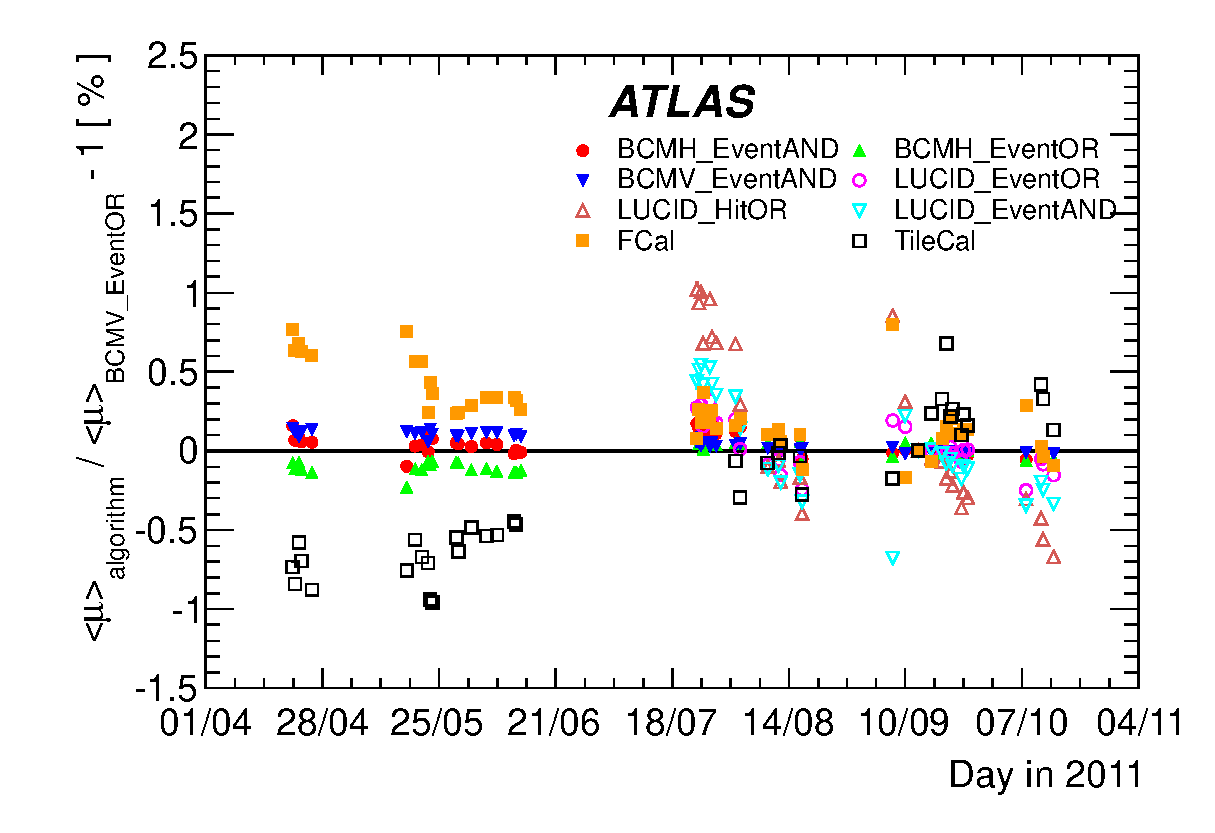
\includegraphics{figures/ch4-reconstruction/luminosity_long_term_stability}}
	}
	\hfill
	\subfloat[] {\label{fig:reco-luminosity-comparisons-pileup}
		\resizebox{0.45\textwidth}{!}{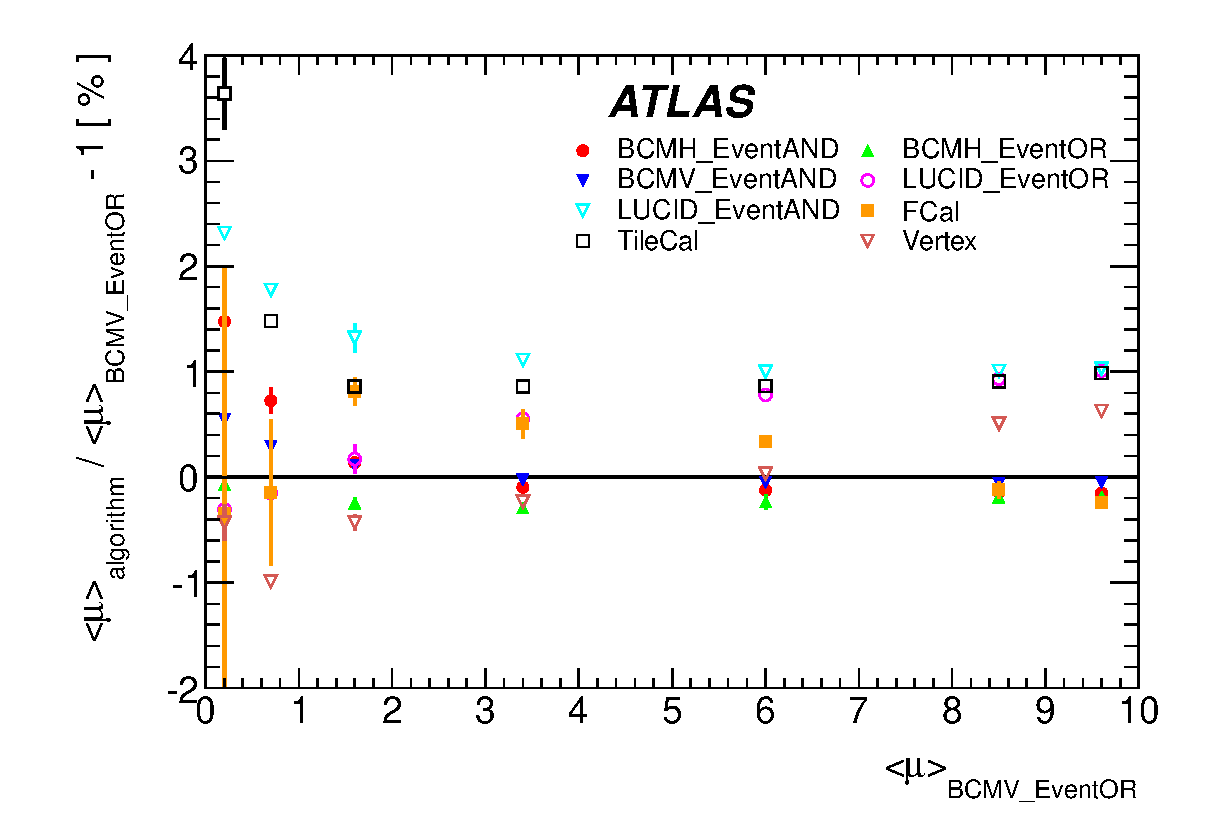
\includegraphics{figures/ch4-reconstruction/luminosity_pileup_muscan}}
	}
	\hfill
	\caption{Left:  Comparison of luminosities measured by different algorithms as a function of time in 2011. Right:  Comparison of luminosities measured by different algorithms as a function of the average number of interactions per bunch cross, $\mu$, as measured by BCM\_VOR. The data were taken during a single run by separating the beams in the transverse direction, similar to a van der Meer scan.}
	\label{fig:reco-luminosity-comparisons}
\end{figure}

\subsection{Vertex-Based Luminosity Measurement}

\subsubsection{Track and Vertex Reconstruction}

Vertices are points consistent with being the origin of a set of tracks reconstructed by the inner detector. The tracks, nominally due to charged particles traversing the inner detector, are reconstructed by a series of algorithms based on hits in inner detector~\cite{TheATLASCollaboration:2010vk}. The algorithm begins by constructing three-dimensional space points associated with the hits in the pixel and SCT layers. Track seeds are formed from sets of three space points in the first four layers of the inner detector (three pixel layers and the innermost SCT layer), constrained to be consistent with a track originating from the interaction region. The track seeds are extended through the remaining SCT layers using a combinatorial Kalman filter. After screening the track candidates to reduce random coincidences and ambiguities from very close tracks, the tracks are extended through the TRT. Finally, the track is refitted using all of the associated hits. 

The vertex reconstruction algorithm reconstructs vertices one by one, alternately finding a vertex seed and then fitting the corresponding tracks. The tracks are required to have $\pt>400 \MeV$, no missing hits where expected (\emph{holes}) in the pixel layers, and at most two holes in the SCT layers. The seed finding identifies the global maximum in the distribution of $z$ coordinates of the tracks. The vertex position is then determined by an adaptive vertex fitting algorithm~\cite{Fruhwirth:2007hz}, a $\chi^2$-based fit which suppresses the contribution from outlier tracks. In most cases, the position of the interaction region is also used as a constraint in the fit; however, for the luminosity measurement using vertices, the constraint is not applied to avoid biases due to changes in the size of the interaction region. Tracks whose impact parameter is inconsistent by more than $7\sigma$ with the vertex position are then reused to seed a new vertex, until no further seeds can be found. 

\subsubsection{Vertex Counting Method}
Vertex counting is an appealing luminosity measurement technique for a number of reasons. The backgrounds are very low, and can be controlled by requiring a minimum number of tracks per vertex, chosen to be at least five tracks in this analysis. Further, the vertex reconstruction efficiency is expected to be stable throughout the data-taking period. However, the technique has two significant drawbacks. First, the data is collected through the standard ATLAS data acquisition system, limiting the rate during normal physics runs to $\mathcal{O}(100~\mbox{Hz})$. Depending on the trigger used, a correction for the trigger deadtime may also be necessary. Second, the efficiency of the vertex reconstruction algorithm is significantly nonlinear with pileup, with the efficiency decreasing by $\sim20\%$ between pileup values of $\mu=1$ and $\mu=30$. 

The nonlinear efficiency with respect to pileup is due to three phenomena:

\begin{itemize}
	\item Vertex masking: a $pp$ interaction fails to be reconstructed as a vertex because some or all of its tracks are used by an earlier vertex in the iterative algorithm. 
	\item Fake vertices: a vertex passes the cut on the minimum number of tracks due to acquiring tracks from another nearby $pp$ interaction.
	\item Split vertices: a single interaction is reconstructed as two separate vertices.
\end{itemize}

Split vertices are a significant effect when considering all vertices with at least two tracks, but is negligible for vertices with at least five tracks. Fake vertices are a subdominant but significant effect. A correction is derived using truth matching in minimum bias Monte Carlo simulation. The simulation sample was generated using \pythia~8, with tune A2M~\cite{pythia}. For a given cut on the minimum number of tracks per vertex, $m$, a reconstructed vertex is labelled as fake if less than $m$ of its tracks are matched to charged particles originating from the same generated $pp$ interaction.

The average number of reconstructed vertices labelled as fake by Monte Carlo truth matching is shown as a function of pileup in figure~\ref{fig:fake-fractions}. The fake fractions show a significant dependence on $\mu$ and on the minimum number of tracks per vertex.

\begin{figure}[h]
	\centering
	\resizebox{5in}{!}{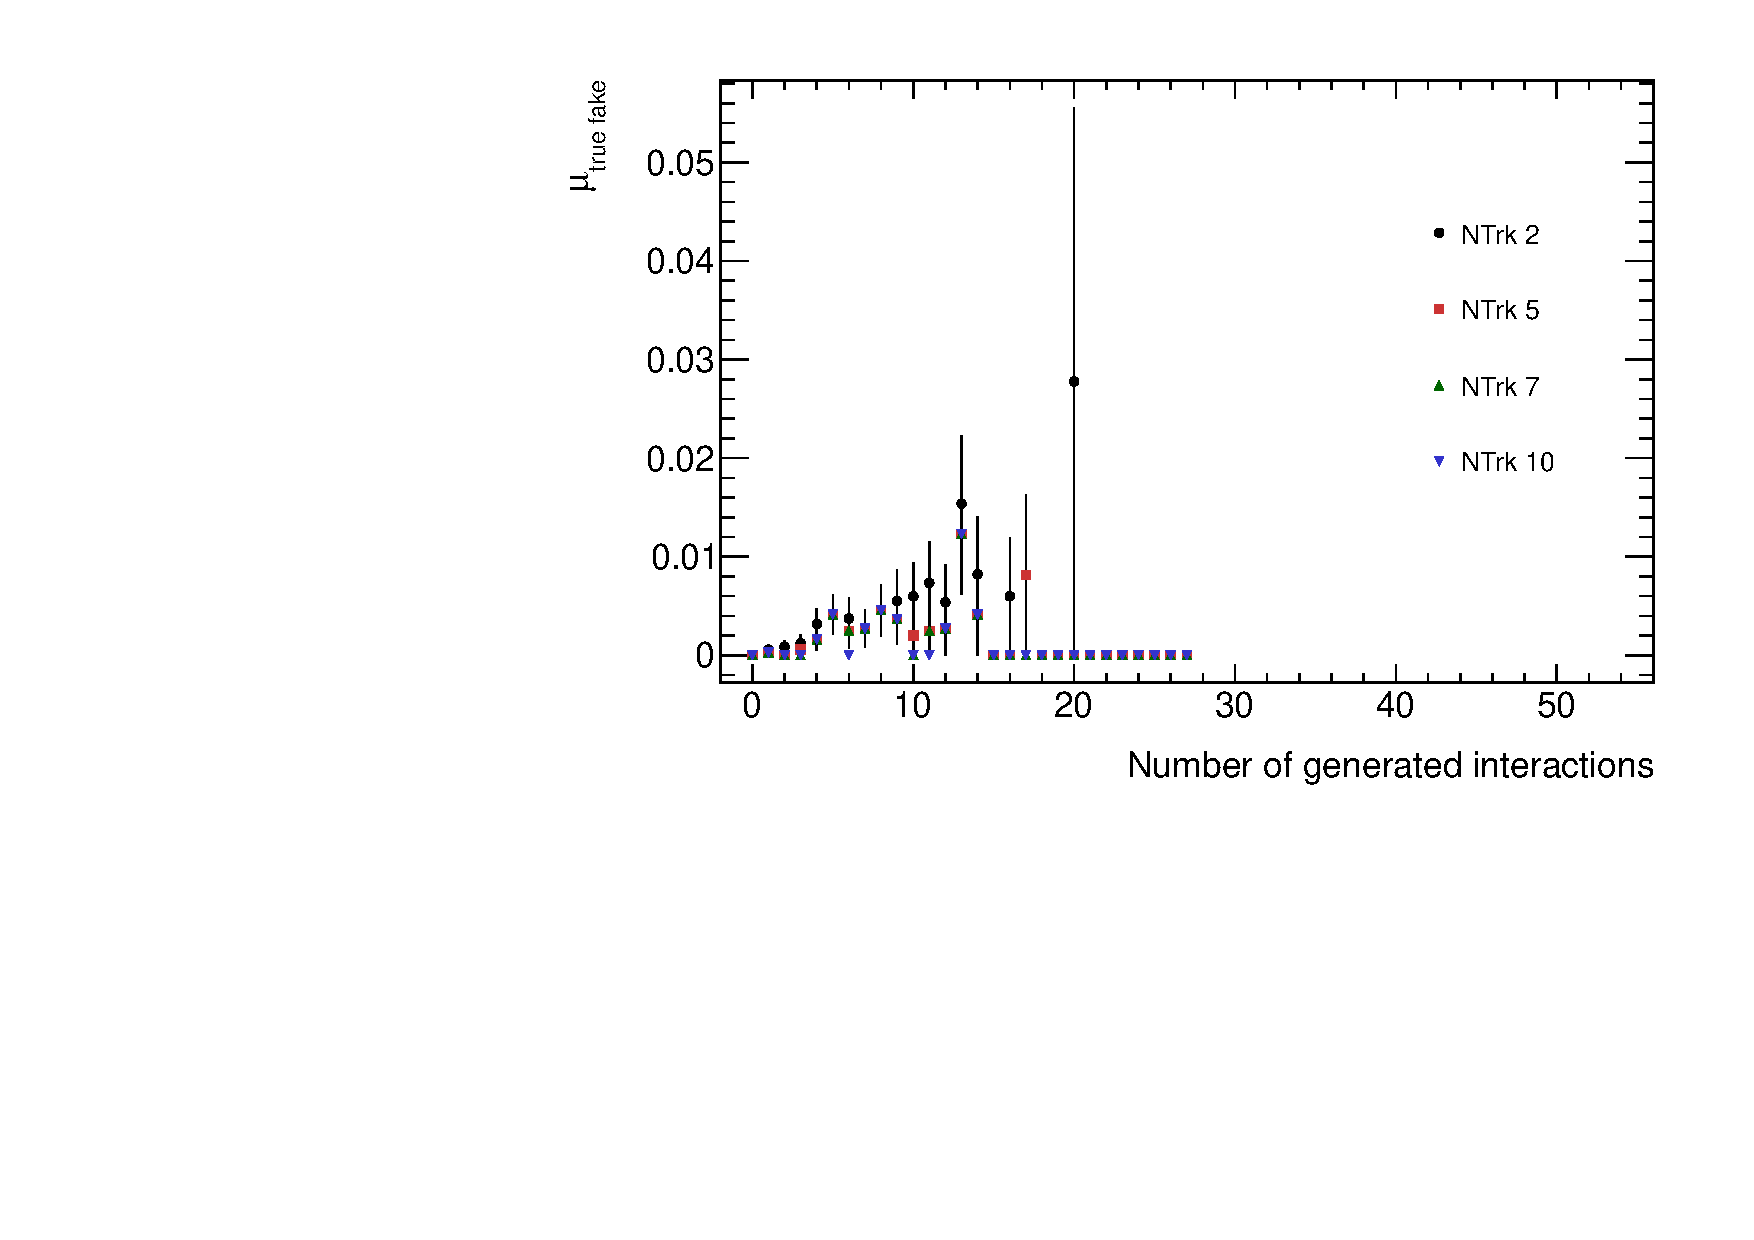
\includegraphics{figures/ch4-reconstruction/c_truefakemu_NGenInt.pdf}}
	\caption{Average number of reconstructed vertices without a matched truth interaction, as a function of number of generated interactions per event. The contribution is below 0.1\%.}
	\label{fig:truefakes}
\end{figure}

\begin{figure}[h]
	\centering
	\subfloat[$\mu_{\textrm{fake}}$ vs. number of generated interactions per event.] {
		\resizebox{3in}{!}{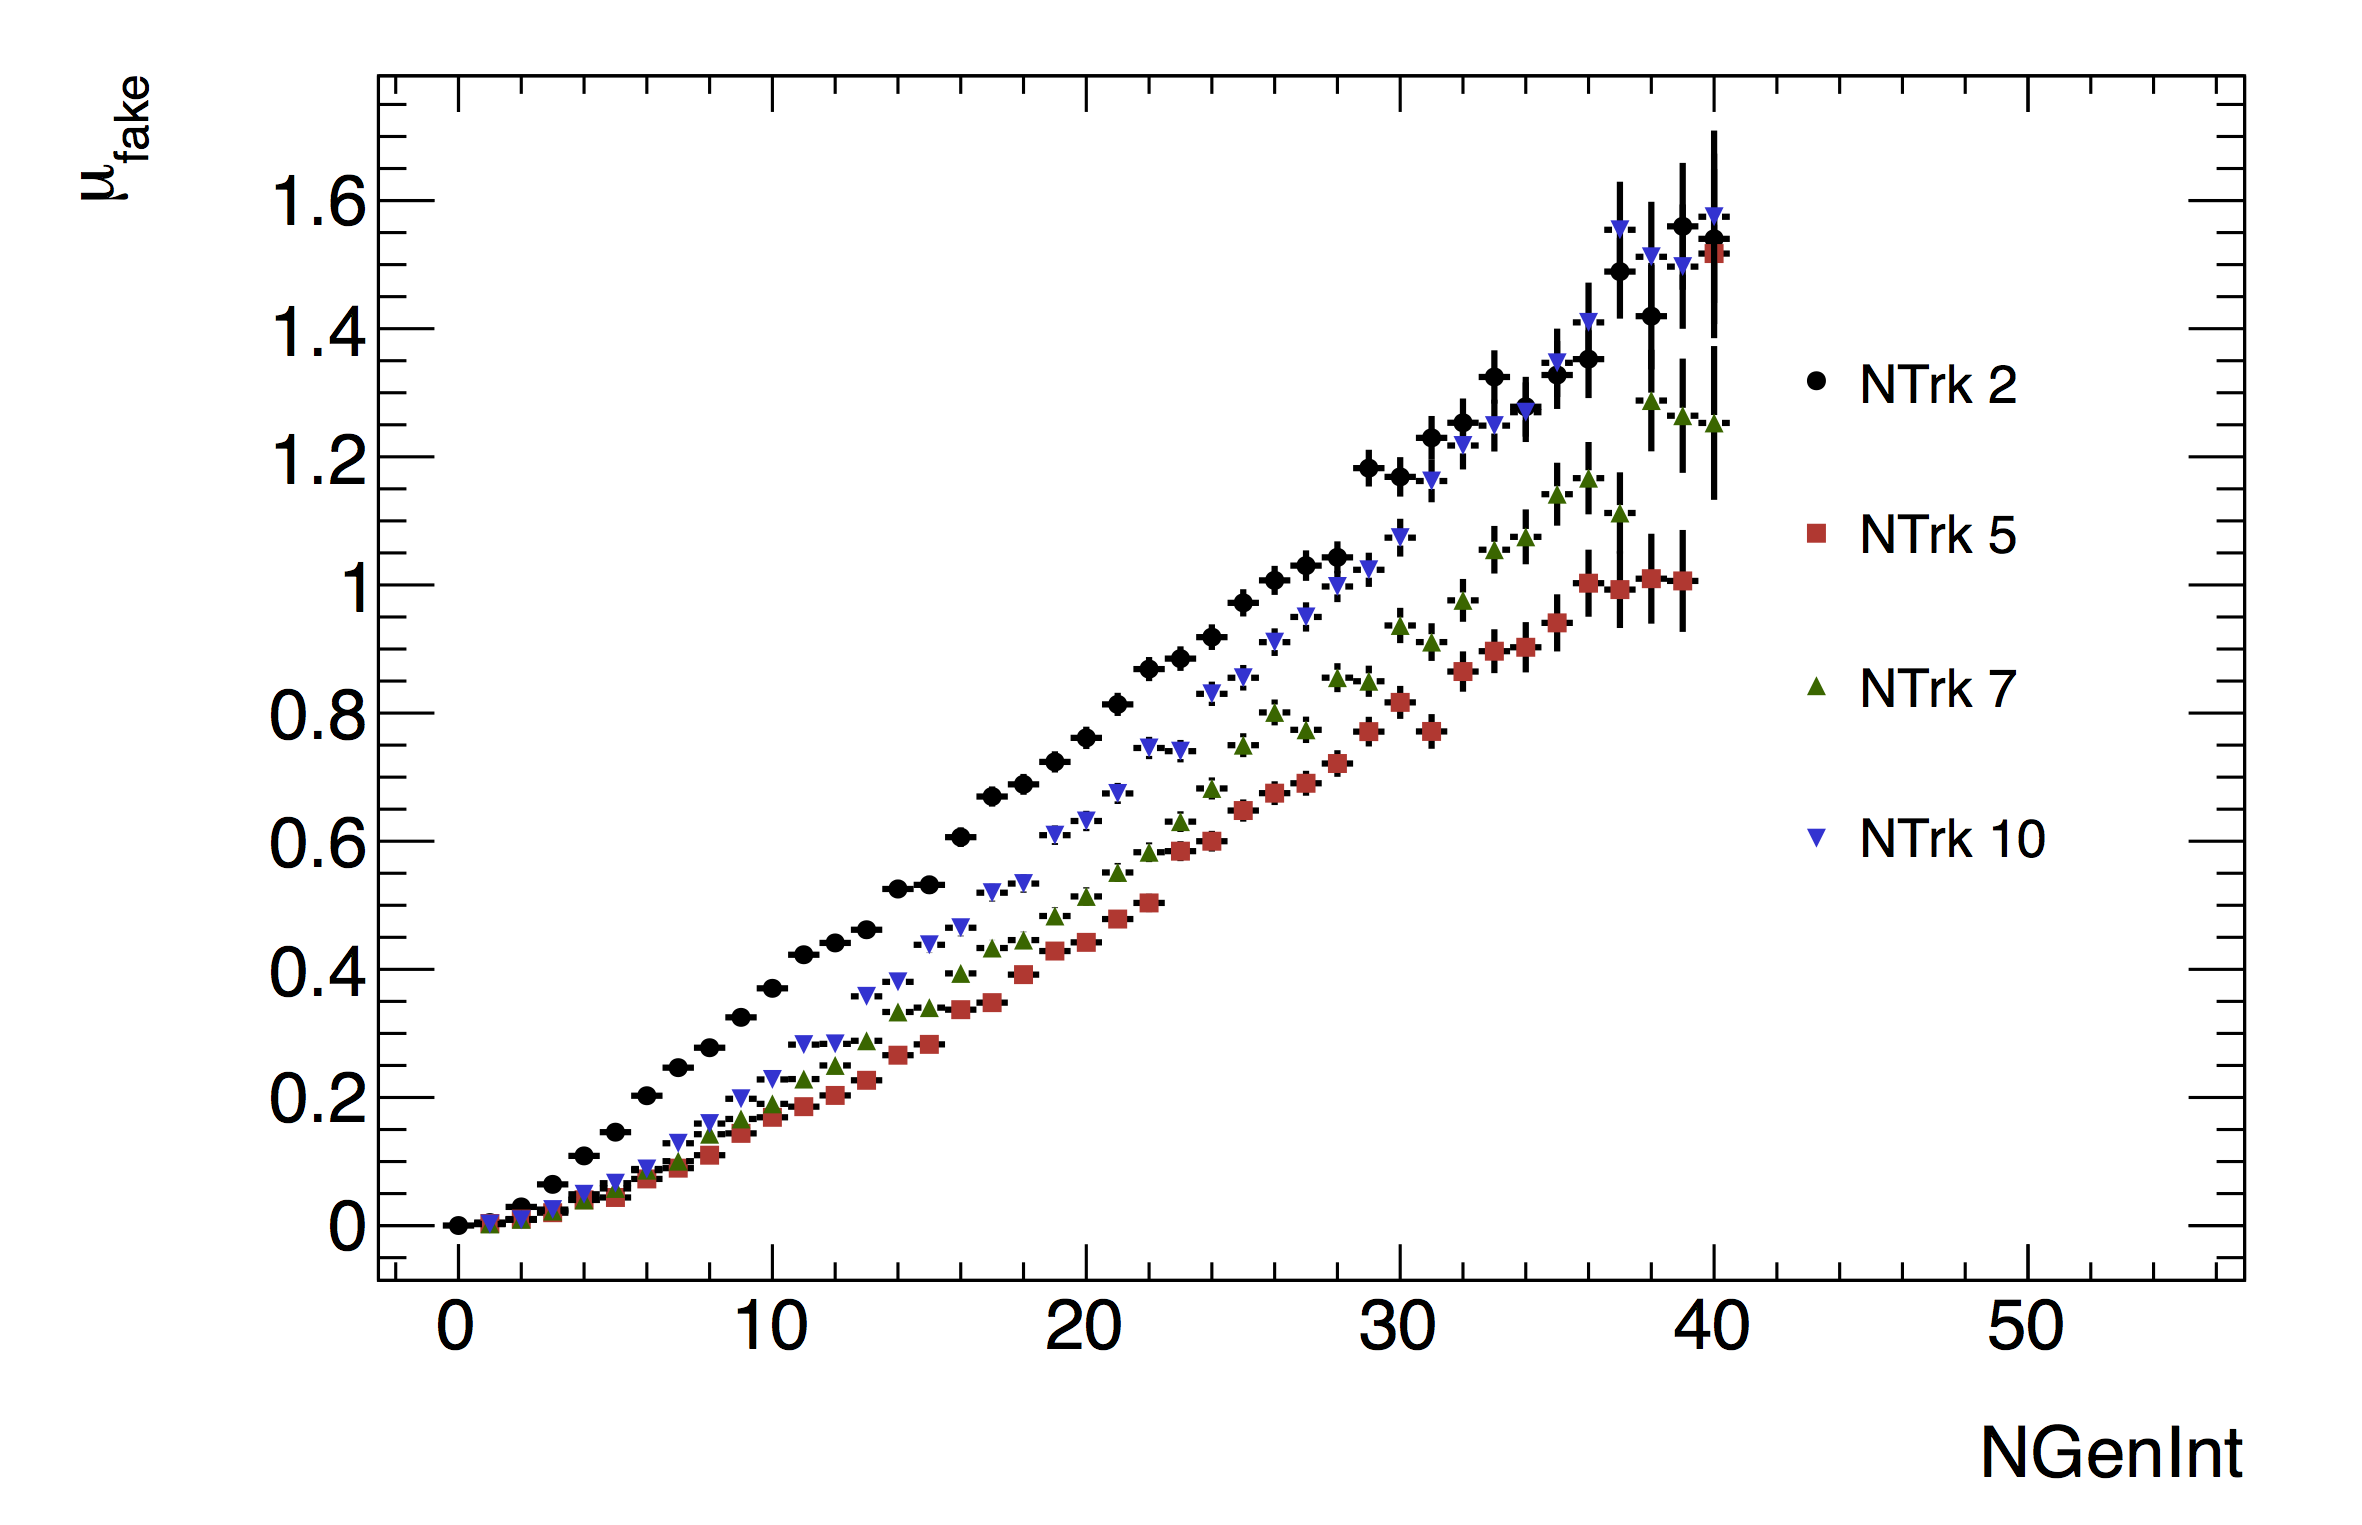
\includegraphics{figures/ch4-reconstruction/c_mu_fake_NGenInt.png}}
	}
	\subfloat[$\mu_{\textrm{fake}}$ vs. $\mu_{\textrm{inel}}$.] {
		\resizebox{3in}{!}{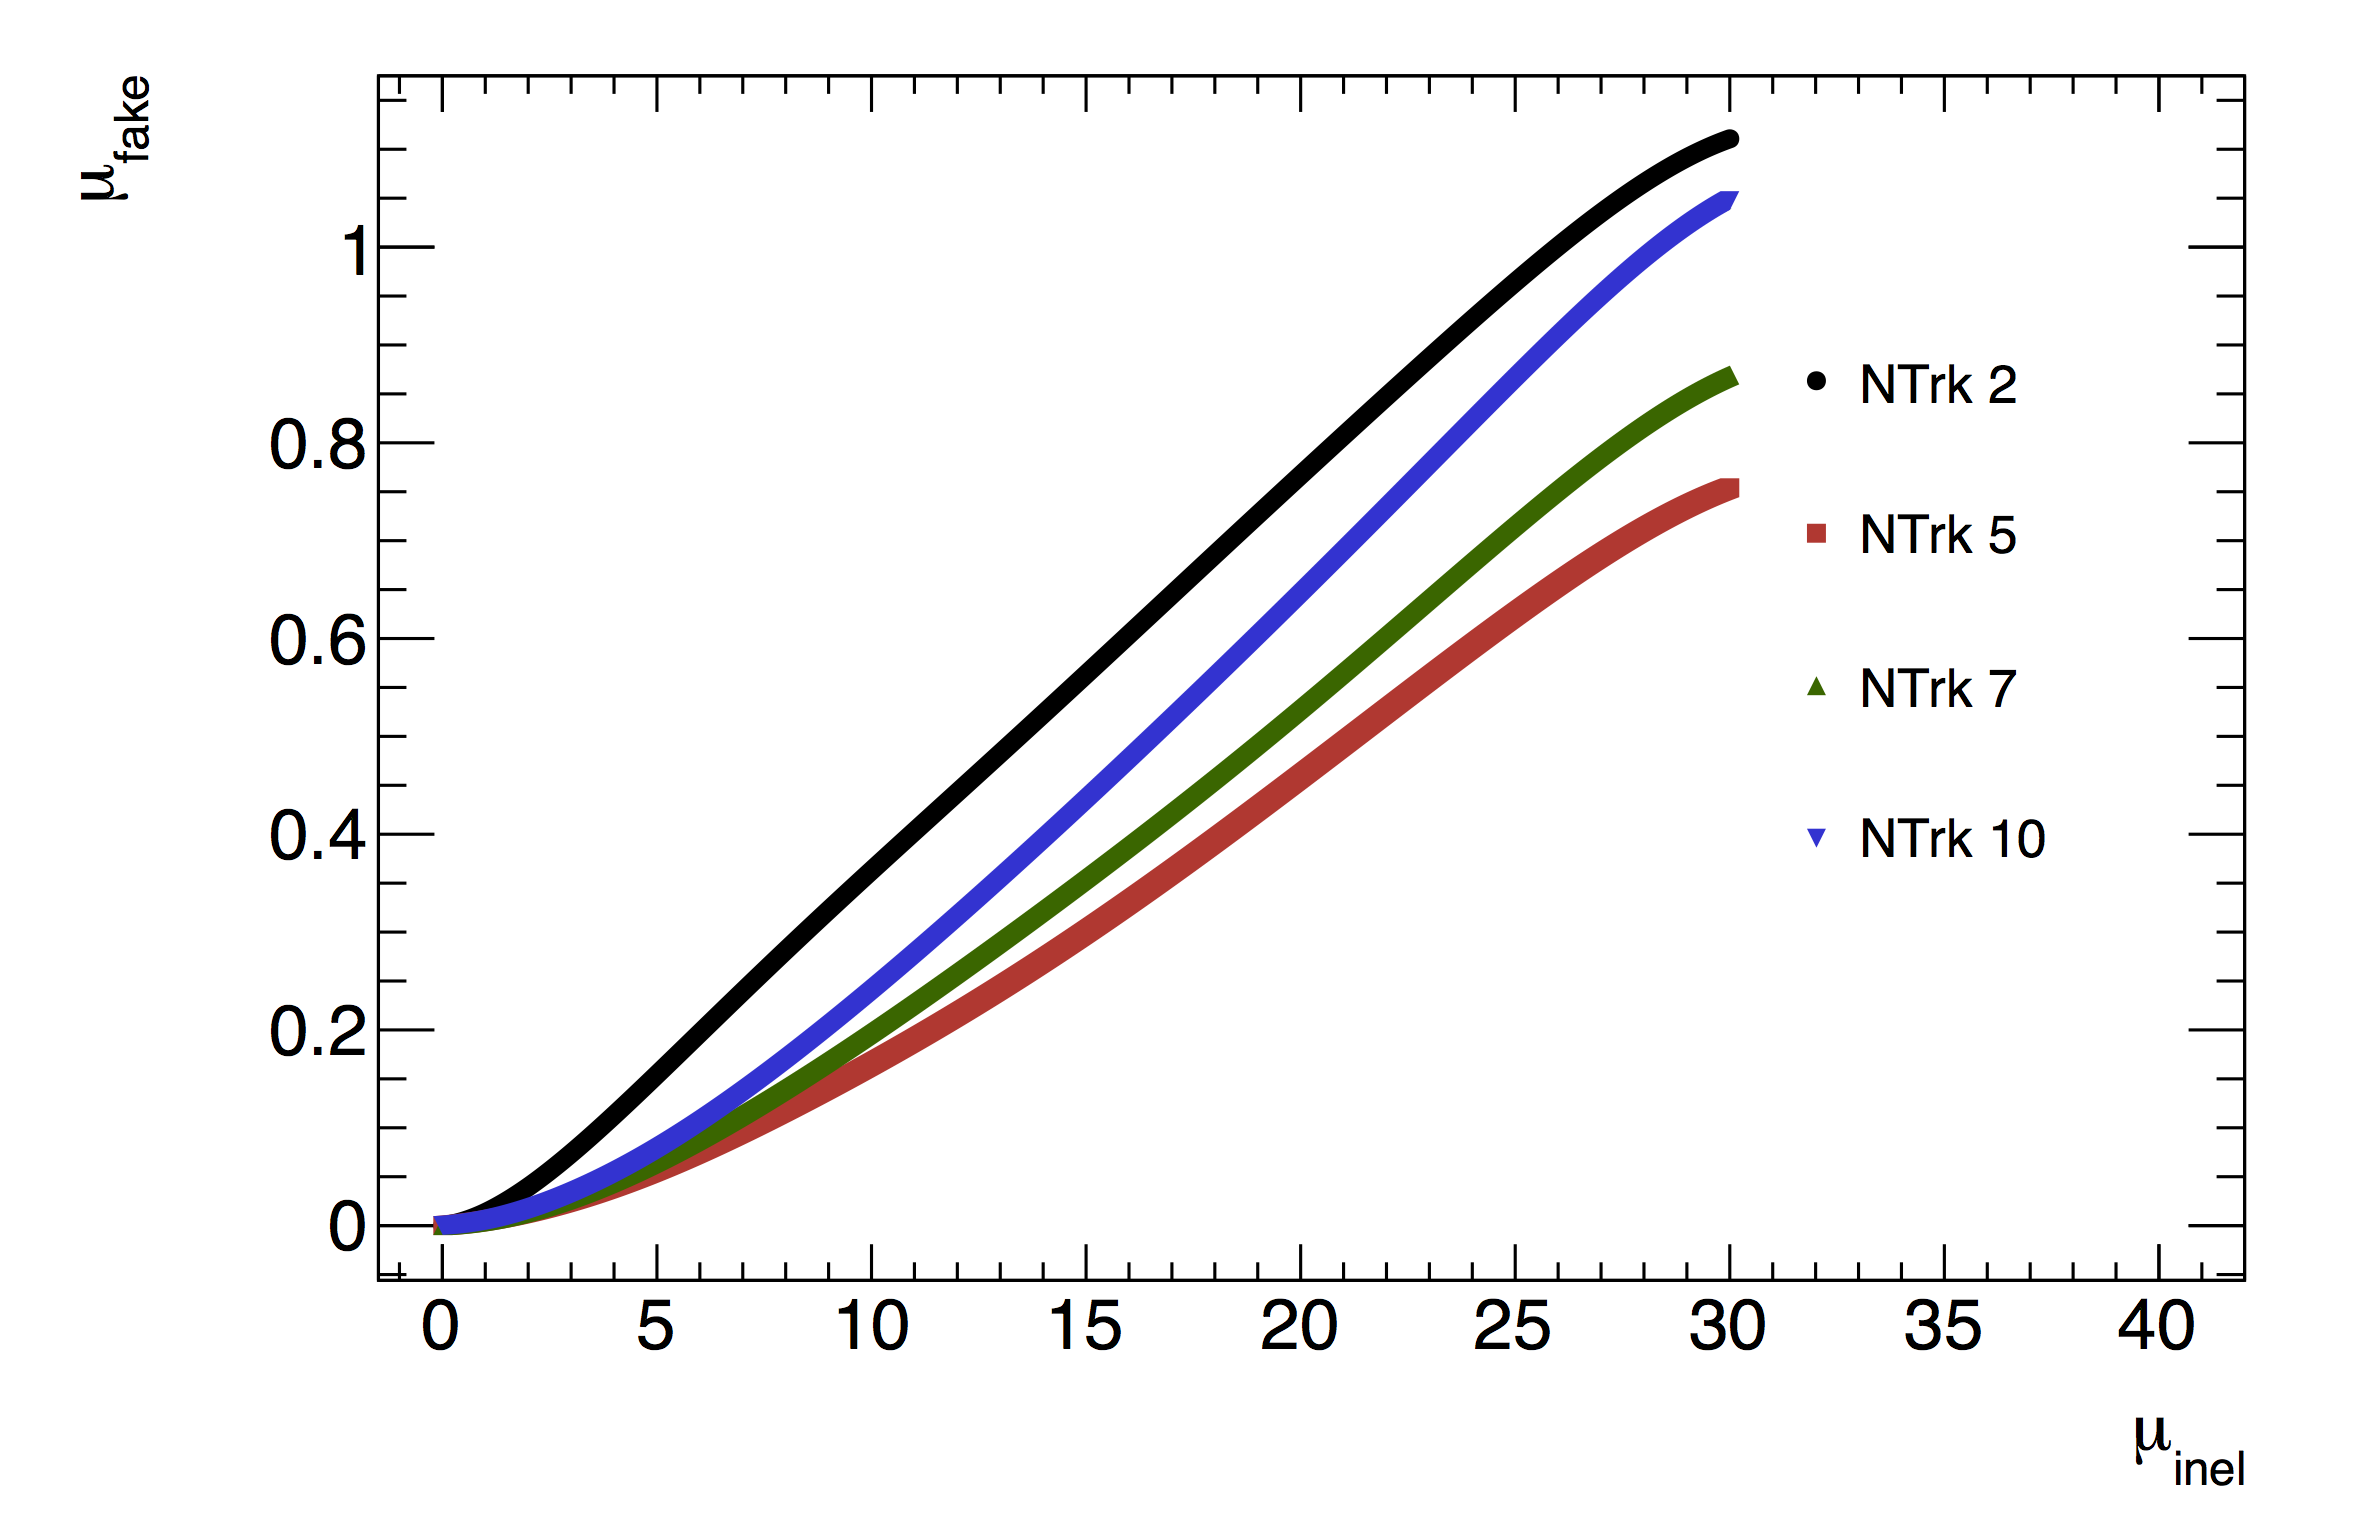
\includegraphics{figures/ch4-reconstruction/c_mu_fake_mu.png}}
	}\\
	\subfloat[$\mu_{\textrm{fake}}$ vs. $\mu_{\textrm{rec}}$ after masking correction.] {
		\resizebox{3in}{!}{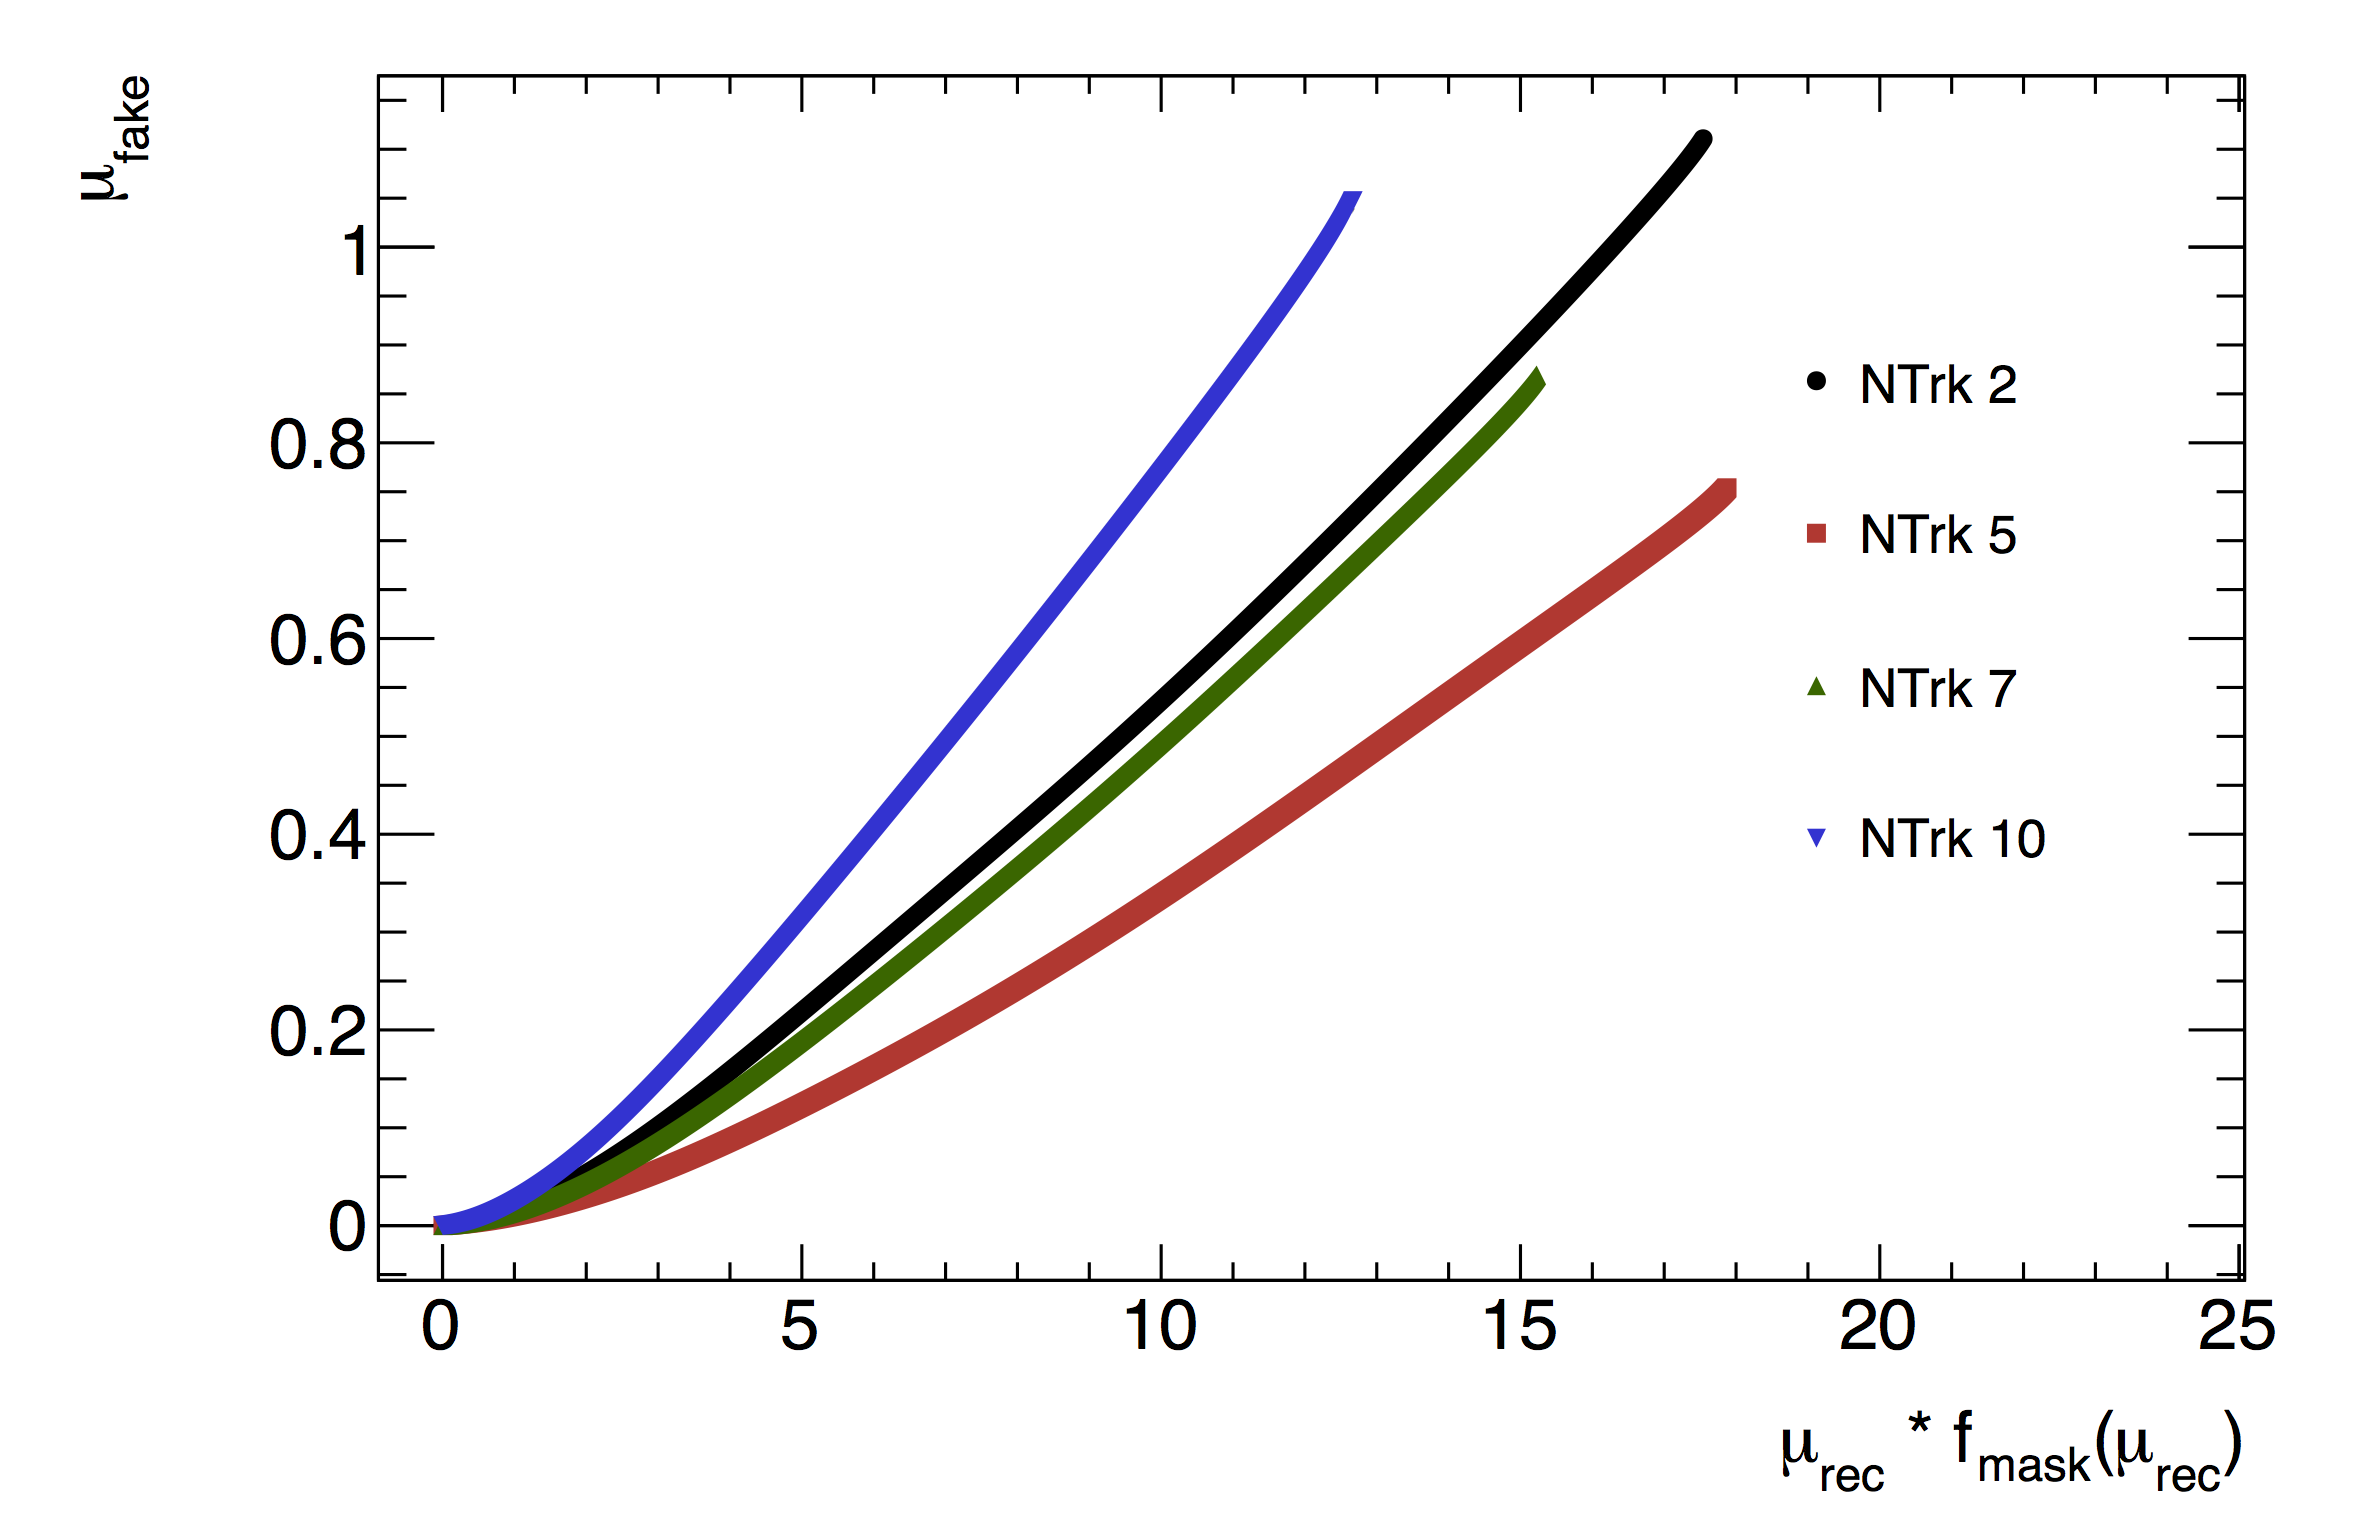
\includegraphics{figures/ch4-reconstruction/c_mu_fake_MuReconMC.png}}
		\label{fig:fake-mu-murecmc}
	}
	\subfloat[$\mu_{\textrm{fake}} / \mu_{\textrm{rec}}$ vs. $\mu_{\textrm{rec}}$ after masking correction.] {
		\resizebox{3in}{!}{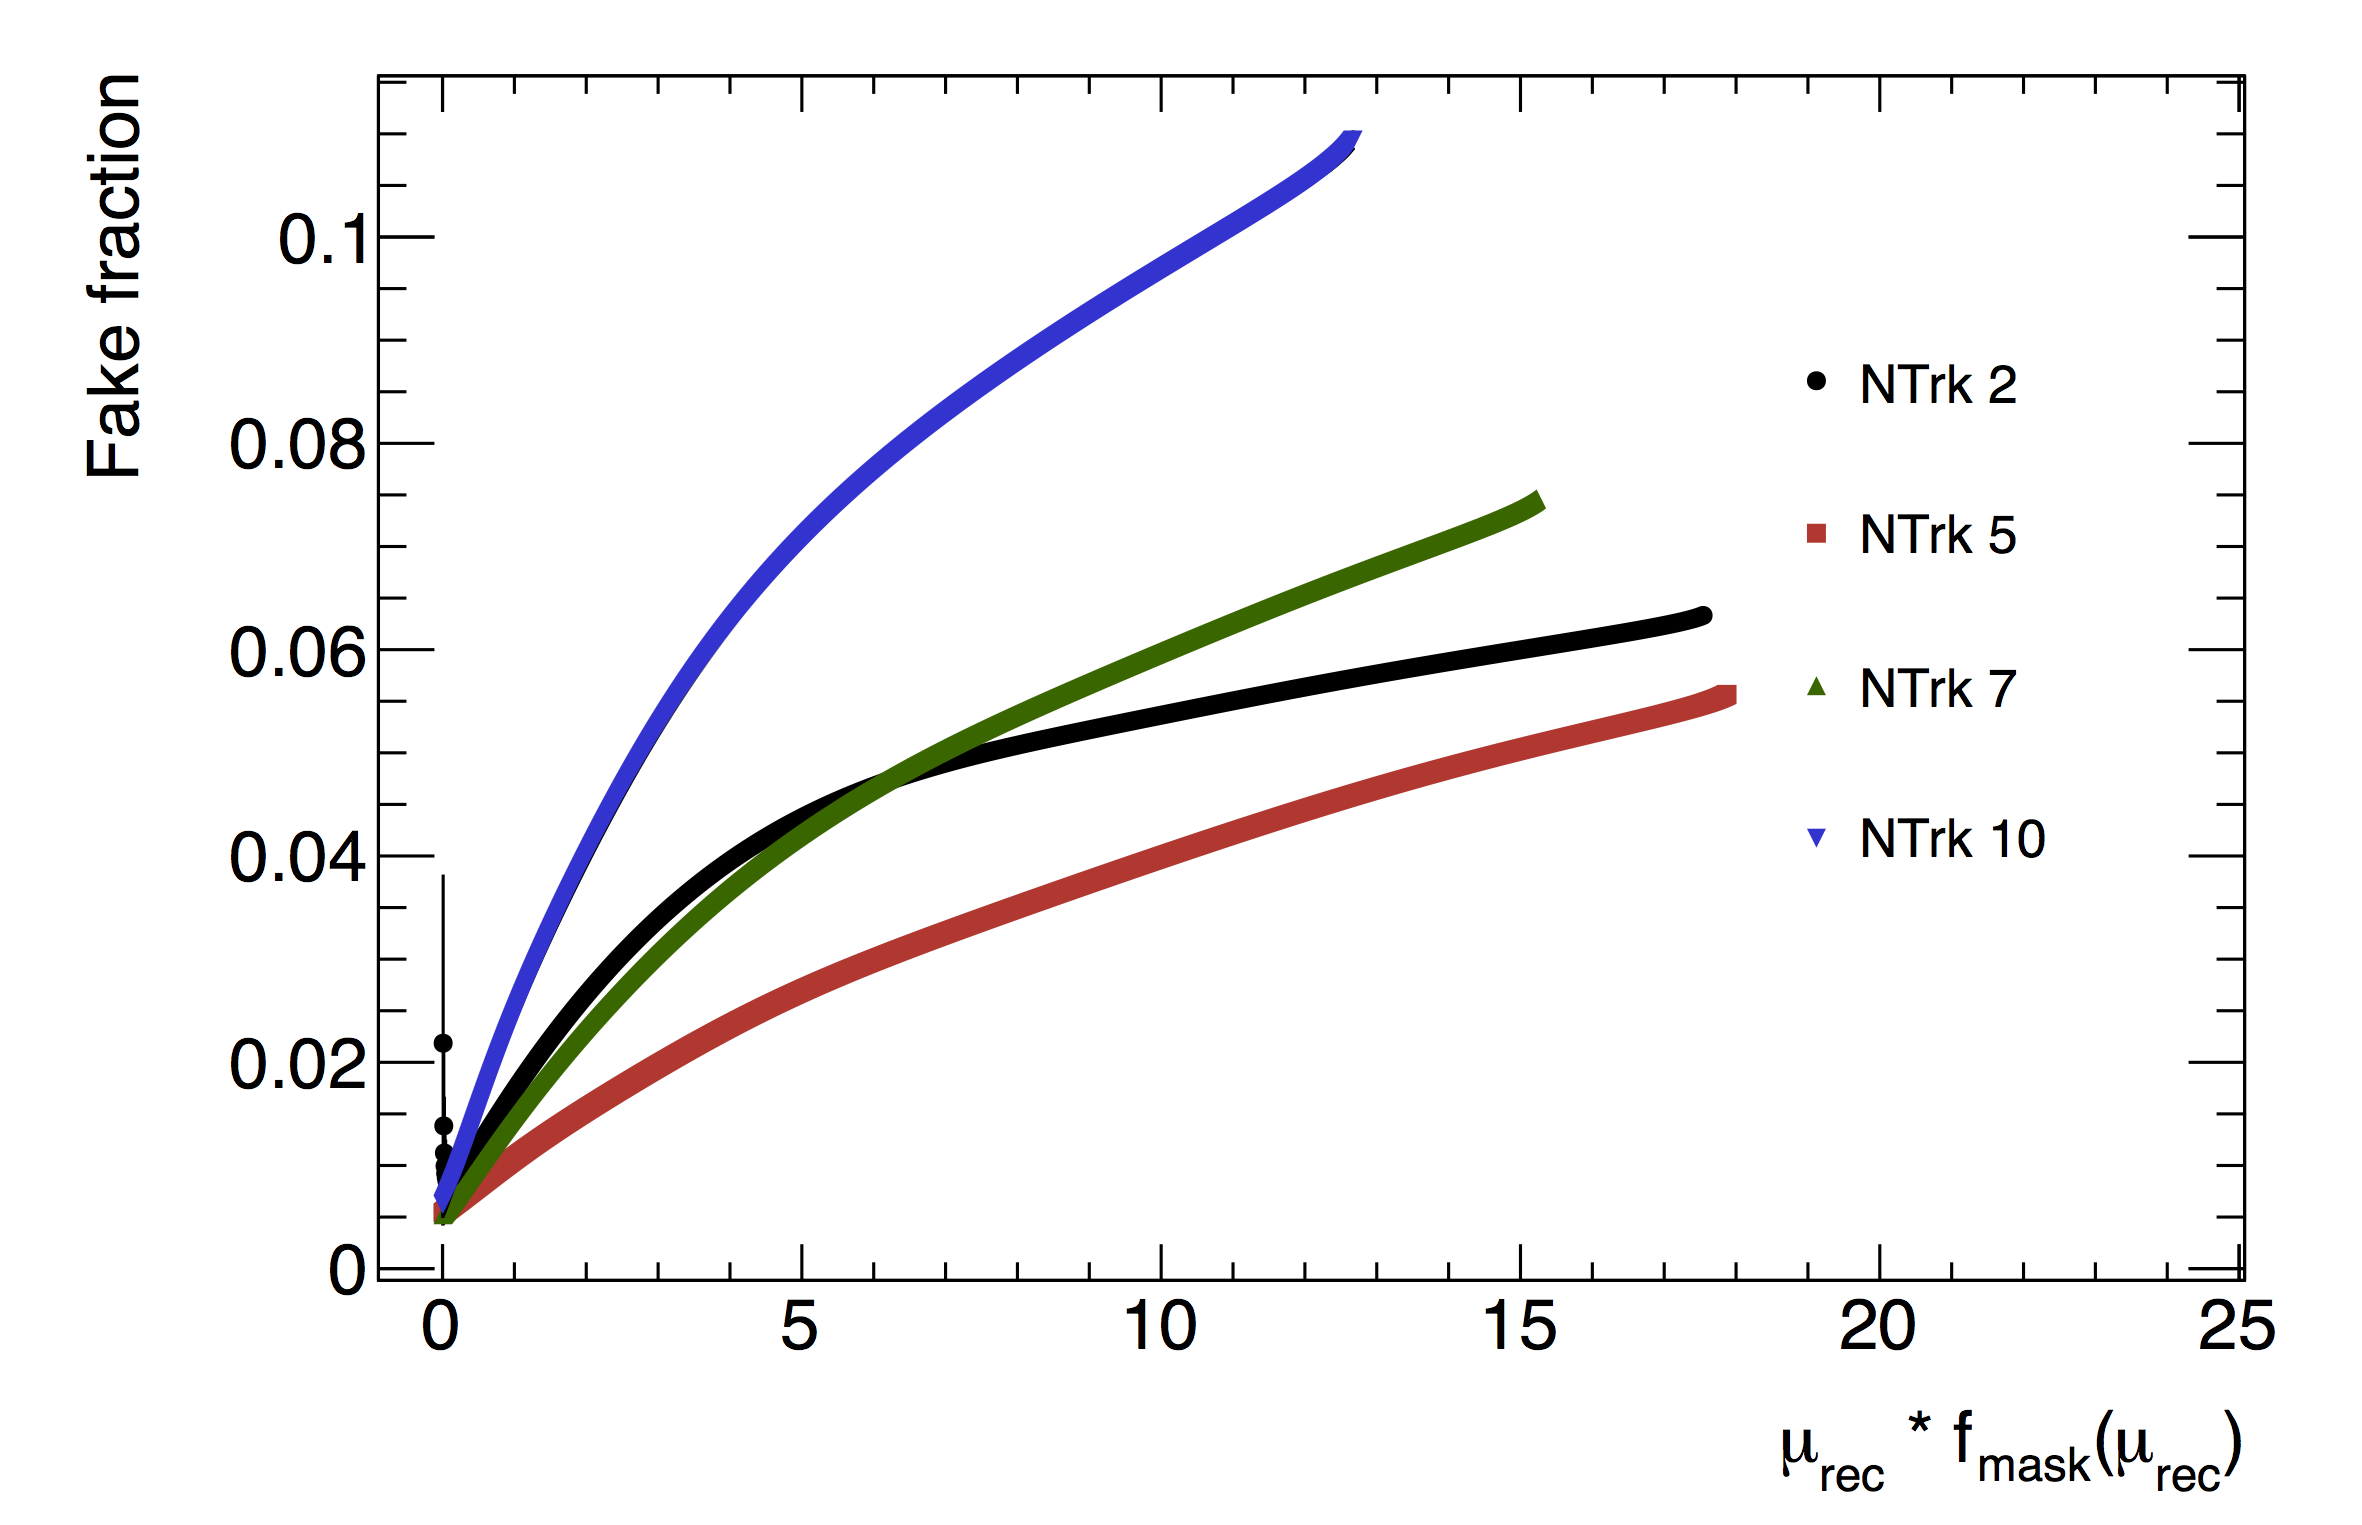
\includegraphics{figures/ch4-reconstruction/c_fake_fraction_MuReconMC.png}}
		\label{fig:fake-fraction-murecmc}
	}
	\caption{Fraction of reconstructed vertices labelled as fake by Monte Carlo truth matching, as a function of pileup.}
	\label{fig:fake-fractions}
\end{figure}


Vertex masking is the dominant effect, causing the large drop in efficiency. Fake vertices are a smaller but significant effect, causing a small increase in the efficiency. Split vertices are a negligible effect once the vertices are required to have at least five tracks. 

A correction procedure is derived for vertex masking using the distribution of longitudinal distances, $\Delta z$, between pairs of vertices in the same event. In the absence of masking, if the interaction region has a Gaussian longitudinal profile with width $\sigma_z$, then the $\Delta z$ distribution would be a Gaussian with width $\sigma_z\times\sqrt{2}$. Masking manifests as an absence of reconstructed pairs near $\Delta z=0$, as shown in figure~\ref{fig:reco-luminosity-deltaz}. 

A correction is derived in a data-driven way as follows. 
\begin{enumerate}
	\item In a data sample with exactly two interactions per event, the number of masked pairs is equal to the number of masked vertices. Using data taken at low pileup values and selecting events with exactly two reconstructed vertices, we calculate the 2-vertex masking probability $p_{\textrm{mask}}(\Delta z)$, i.e. the probability that only one of two vertices separated by $\Delta z$ is reconstructed. This function is assumed to be a universal property of the vertexing algorithm, independent of $\mu$. 
	
	Specifically, the expected $\Delta z$ distribution in the absence of masking, $f_{\mathrm{exp}}(\Delta z)$, is derived by randomly sampling pairs of points from the observed $z$-distribution of reconstructed vertices. Using $f_{\mathrm{exp}}(\Delta z)$ as a template, the \emph{observed} $\Delta z$ distribution, $f_{\mathrm{obs}}(\Delta z)$, is fitted in the range $30$mm$\leq| \Delta z| \leq 300$mm, where vertex masking is negligible. Finally, the masking probability is defined as:
	\begin{equation}
		p_{\textrm{mask}}(\Delta z) = \frac{f_{\mathrm{exp}}(\Delta z) - f_{\mathrm{obs}}(\Delta z)}{f_{\mathrm{exp}}(\Delta z)}
	\end{equation}
	
	The masking probability functions derived from minimum bias Monte Carlo and for low-$\mu$ data are shown in figures~\ref{fig:masking-correction-data} and \ref{fig:masking-correction-mc}.
		
	\item To derive a correction for a particular data sample at arbitrary $\mu$, an \emph{expected} $\Delta z$ distribution, $f_{\mathrm{exp}}(\Delta z)$, is again derived by randomly sample pairs of vertices from the observed primary vertex $z$-distribution. Then, the total probability $p_{\textrm{mask}}$ that given any two tight vertices, only one is reconstructed can be computed: 
	\begin{equation}
		p_{\textrm{mask}} = \int_{-\infty}^{\infty} p_{\textrm{mask}}(\Delta z) f_{\mathrm{exp}}(\Delta z) d(\Delta z).
	\end{equation}
	
	\item The total masking probability $p_{\textrm{mask}}$ is used to generate a map between the number of reconstructible vertices per event, $N_{\textrm{vis}}$, and the average number of reconstructed vertices per event, $\mu_{\textrm{rec}}$, as follows. Label the generated vertices $v_i$, $1 \leq i \leq N_{gen}$, in the order in which the iterative vertexing algorithm reconstructs the vertices; similarly, let $p_i$, $1\leq i \leq N_{\textrm{vis}}$, be the probability that vertex $v_i$ is reconstructed. Proceeding vertex-by-vertex, the $p_i$ follow a recursion relation:

	\begin{align}
		p_1 &= 1\\
		p_2 &= p_1 \times (1 - p_{\textrm{mask}})\\
		&... \\
		p_k &= \prod_{i=1}^{k-1} \left( p_i  \times (1-p_{\textrm{mask}}) + (1-p_i) \times 1\right)\\
		&= \prod_{i=1}^{k-1} \left(1 - p_i p_{\textrm{mask}}\right)\\
		&= p_{n-1} \times \left(1-p_{n-1} p_{\textrm{mask}}\right)
	\end{align}
	The average number of reconstructed vertices is then:
	\begin{align}
		\langle N_{\textrm{rec}} \rangle &= \sum_{i=1}^{N_{\textrm{vis}}} p_i.
	\end{align}
	
	\item Finally, a map is computed between the average number of reconstructible vertices, $\mu_{\textrm{vis}}$, and the average number of reconstructed vertices, $ \mu_{\textrm{rec}}(\mu_{\textrm{vis}})$, by convoluting $\mu_{\textrm{rec}}(N_{\textrm{vis}})$ with a Poisson distribution:
	\begin{align}
		\langle \mu_{\textrm{rec}} \rangle (\mu_{\textrm{vis}}) = \sum_{N_{\textrm{vis}}=0}^{\infty} P(N_{\textrm{vis}}; \mu_{\textrm{vis}}) \mu_{\textrm{rec}} (N_{\textrm{vis}}).
	\end{align}
\end{enumerate}

\begin{figure}[p]
	\centering
	\subfloat[$\Delta z$ distribution and template fit, NTrk5, BCID 81] {
		\resizebox{3in}{!}{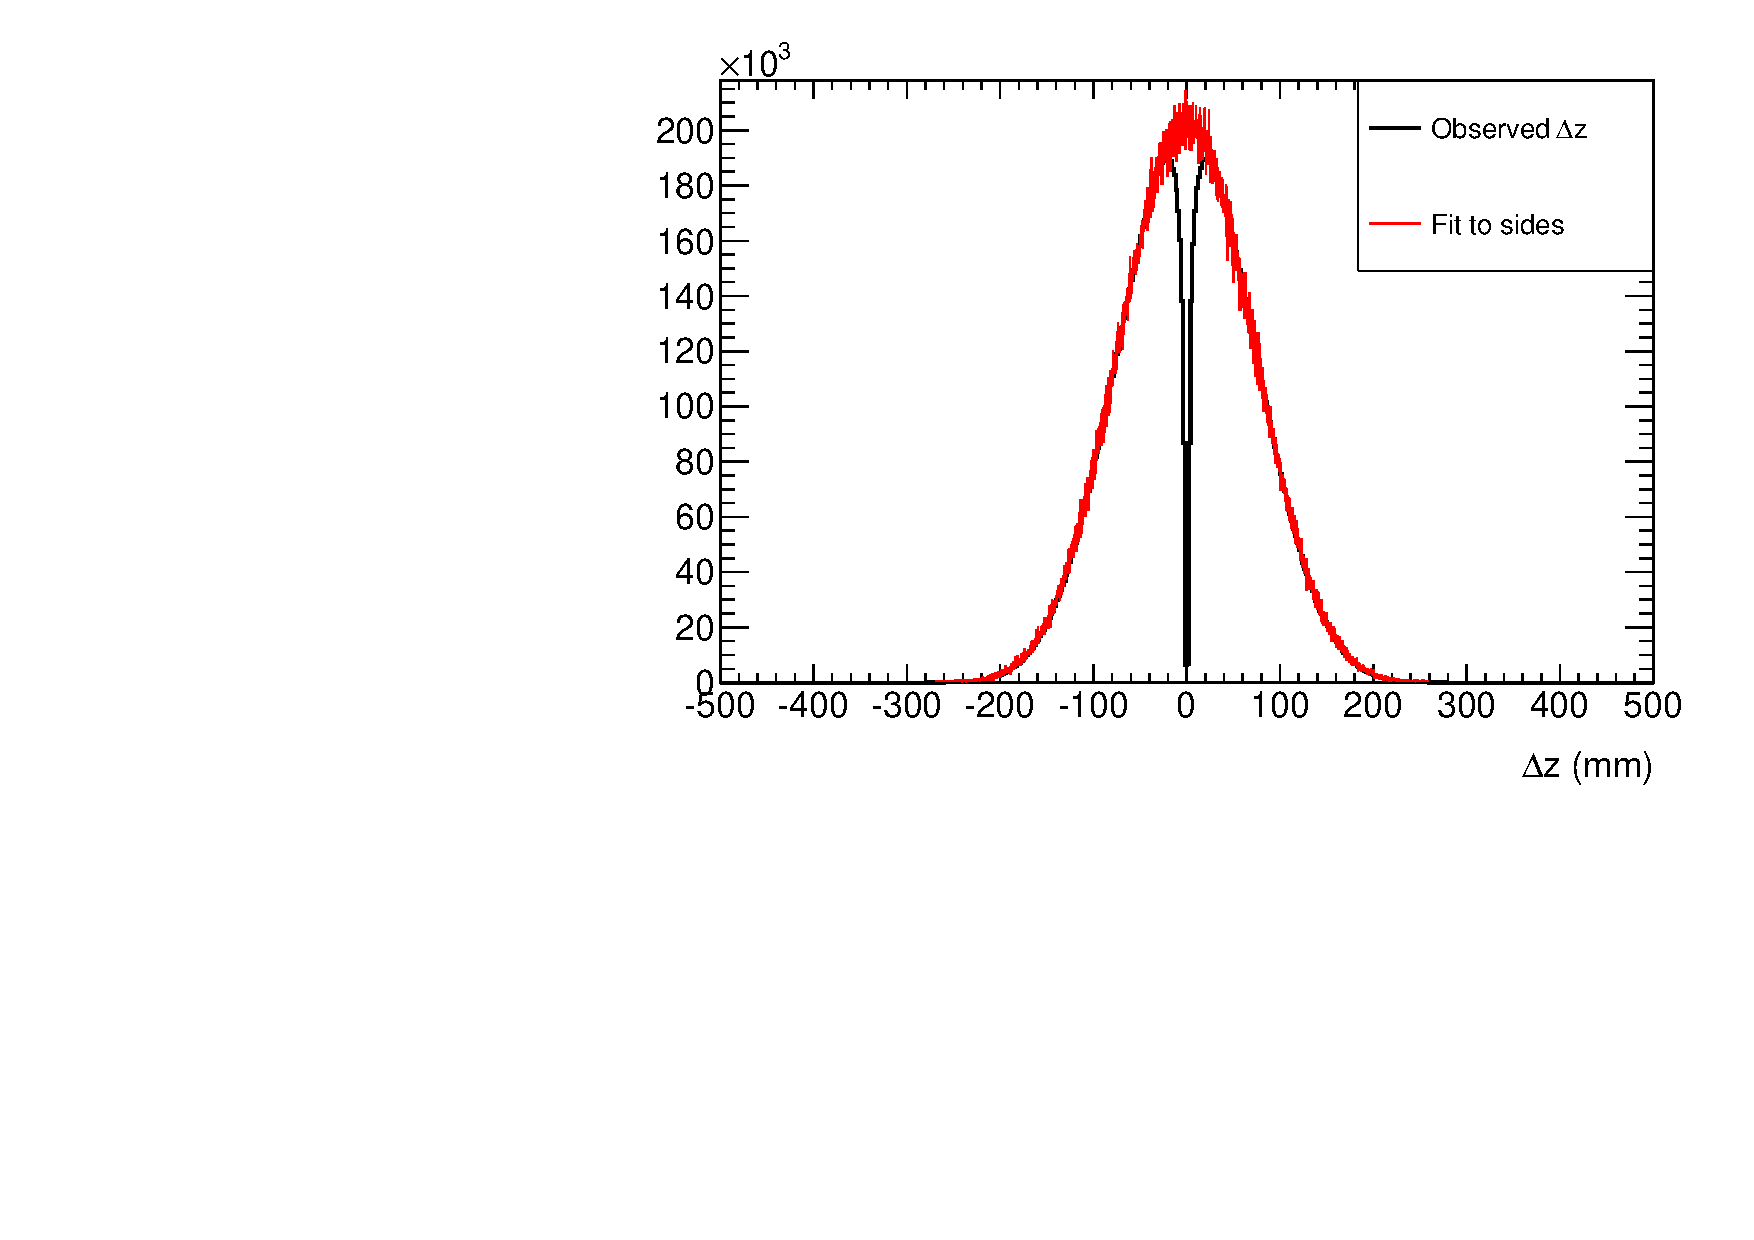
\includegraphics{figures/ch4-reconstruction/c_dz_NTrk5_BCID81}}
	}
	\subfloat[$p_{\textrm{mask}}(\Delta z)$, NTrk5] {
		\resizebox{3in}{!}{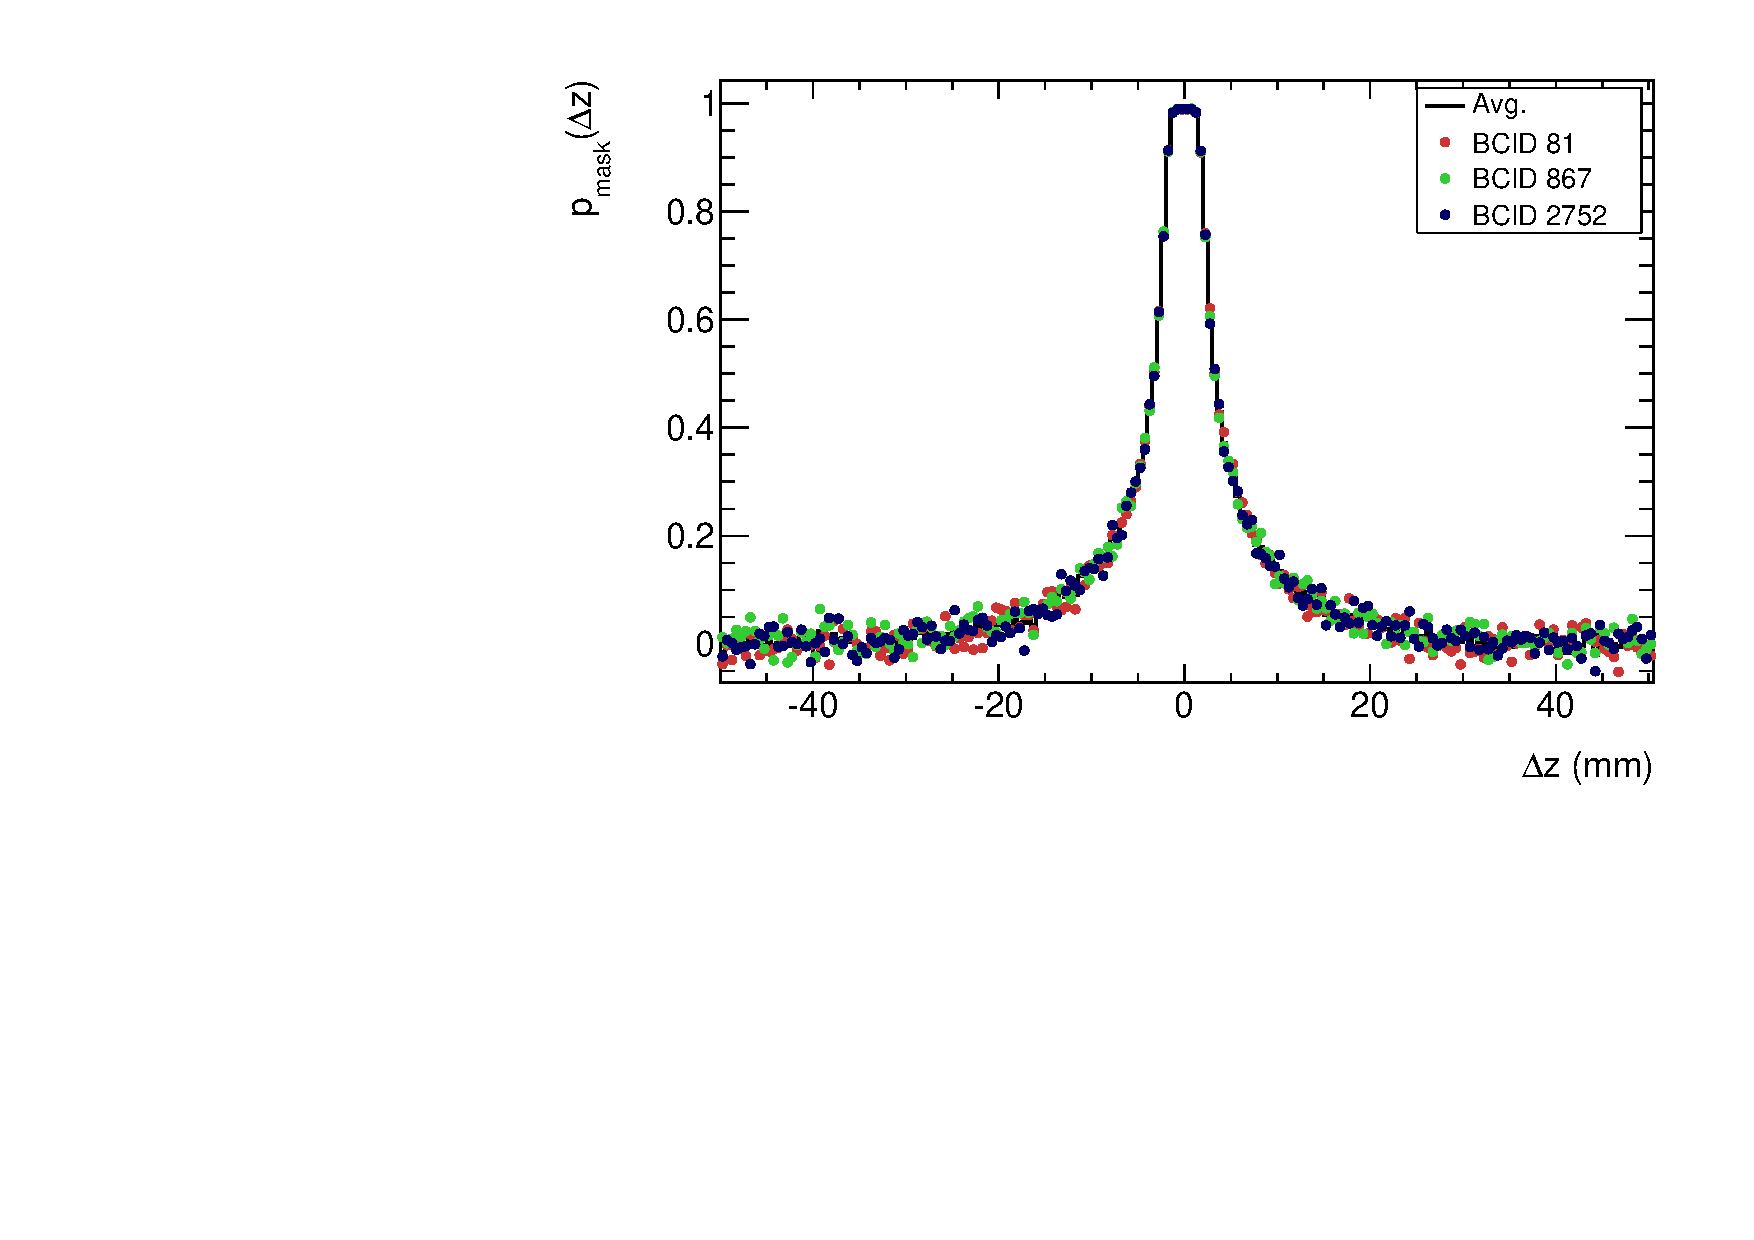
\includegraphics{figures/ch4-reconstruction/c_pmask_dz_NTrk5}}
	}\\
	\subfloat[$\Delta z$ distribution and template fit, NTrk7, BCID 81] {
		\resizebox{3in}{!}{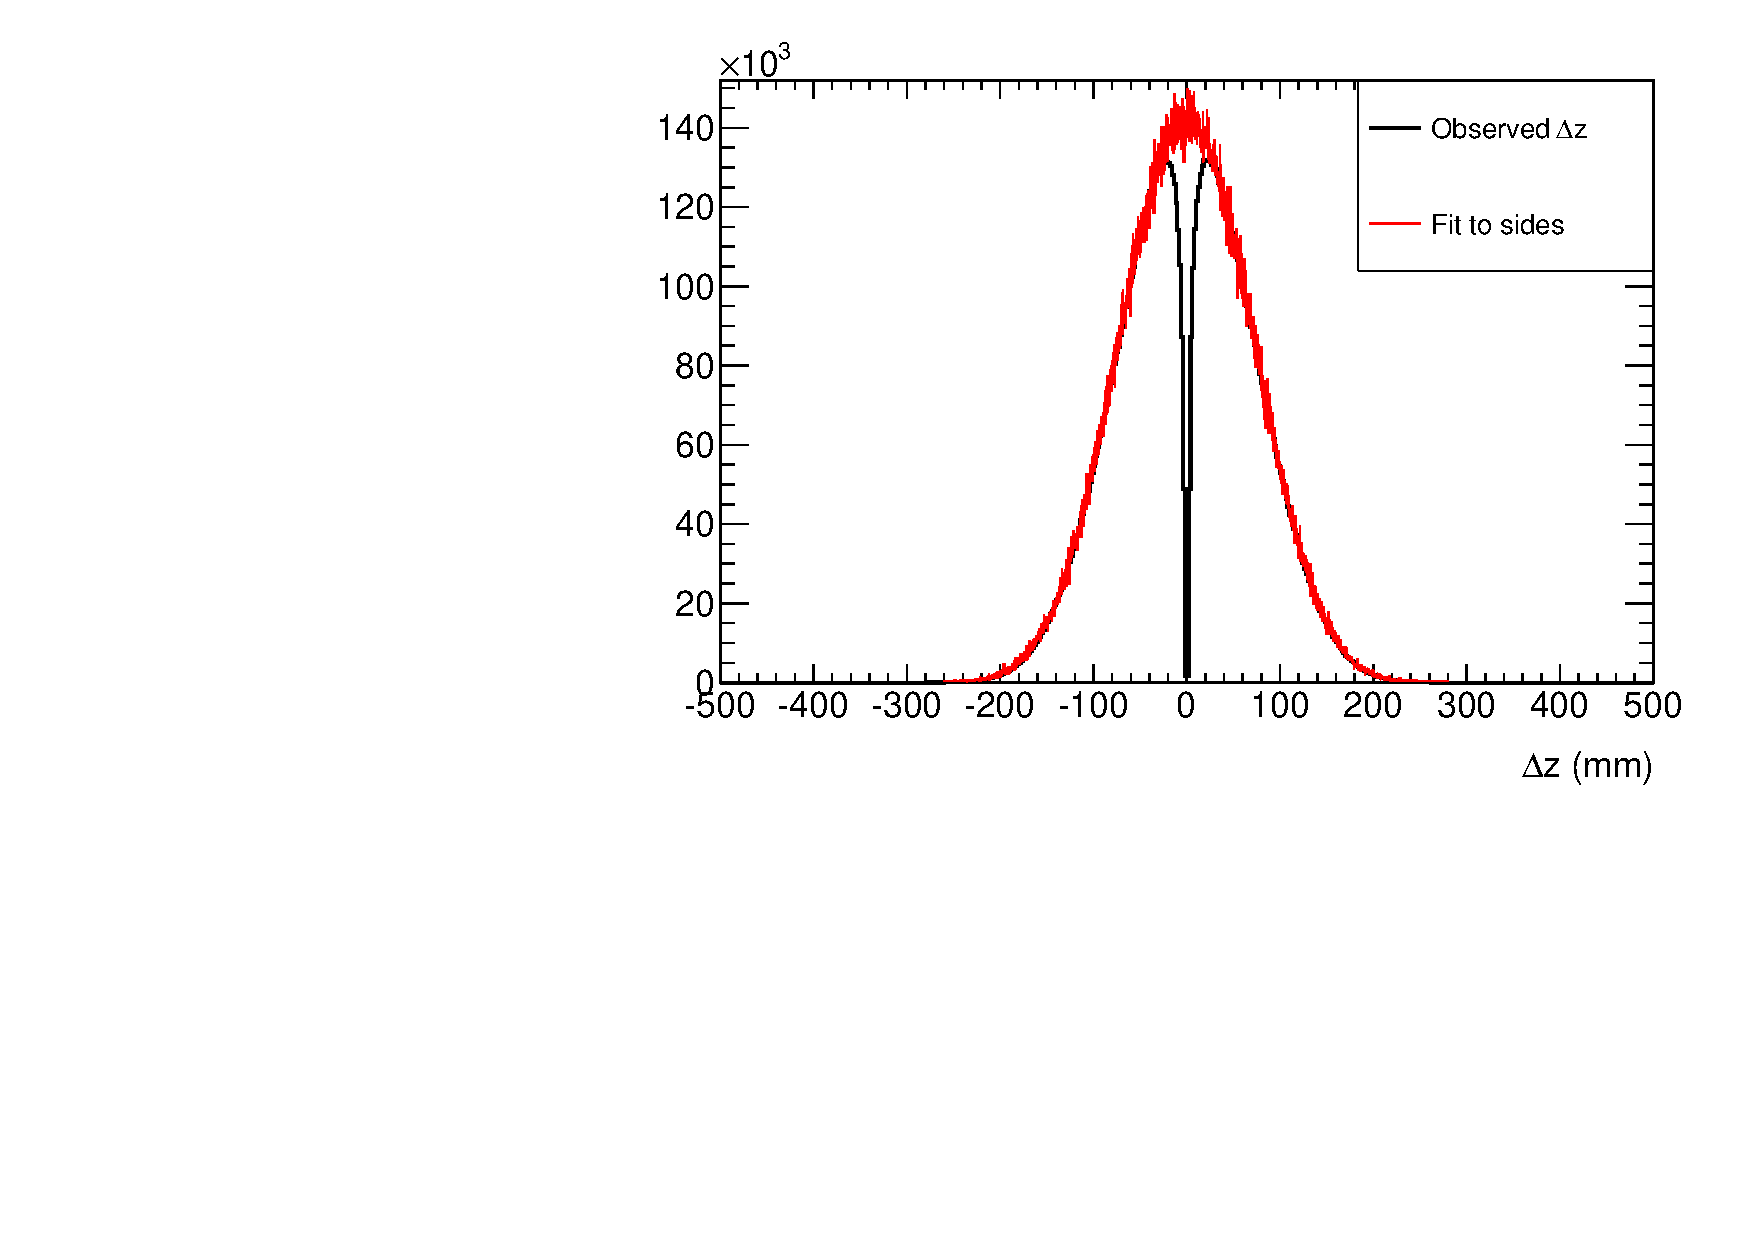
\includegraphics{figures/ch4-reconstruction/c_dz_NTrk7_BCID81}}
	}
	\subfloat[$p_{\textrm{mask}}(\Delta z)$, NTrk7] {
		\resizebox{3in}{!}{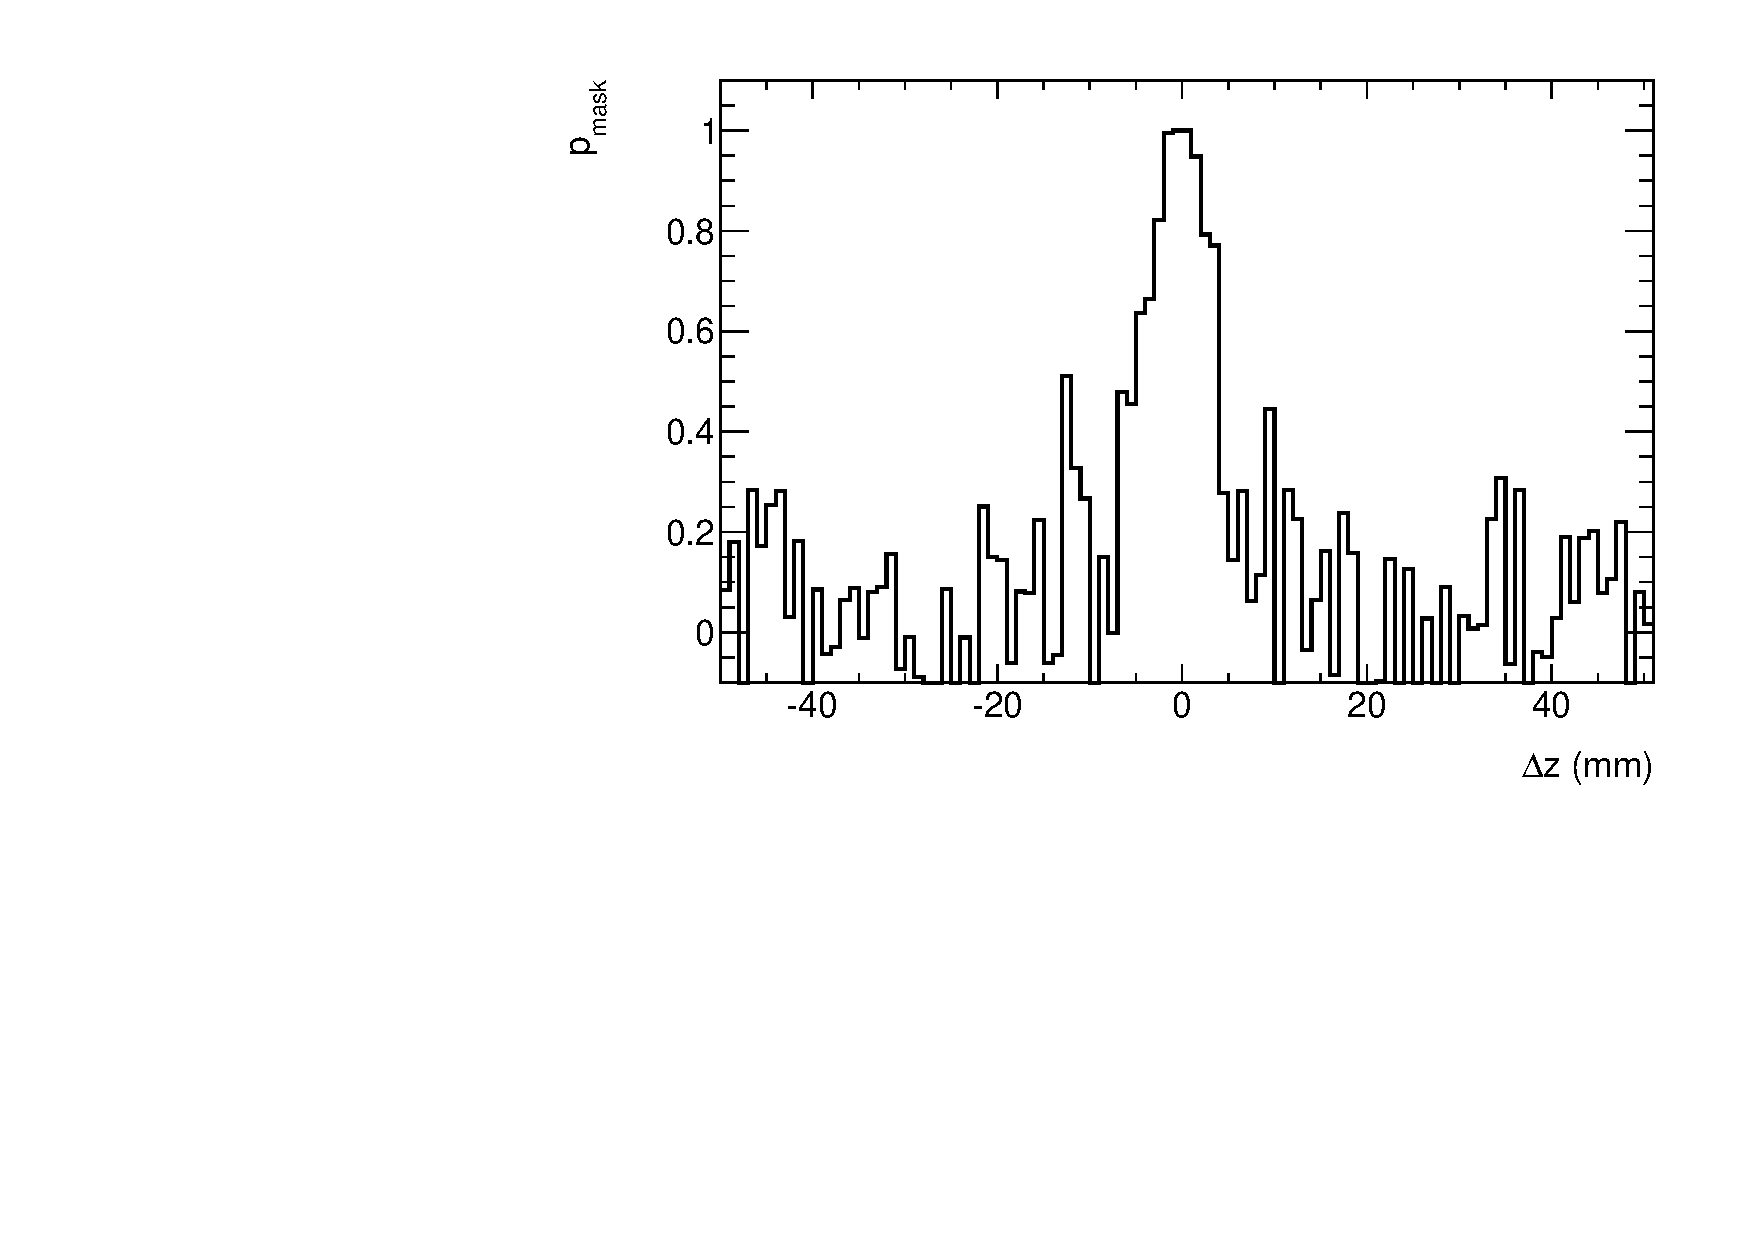
\includegraphics{figures/ch4-reconstruction/c_pmask_dz_NTrk7}}
	}\\
	\subfloat[$\Delta z$ distribution and template fit, NTrk10, BCID 81] {
		\resizebox{3in}{!}{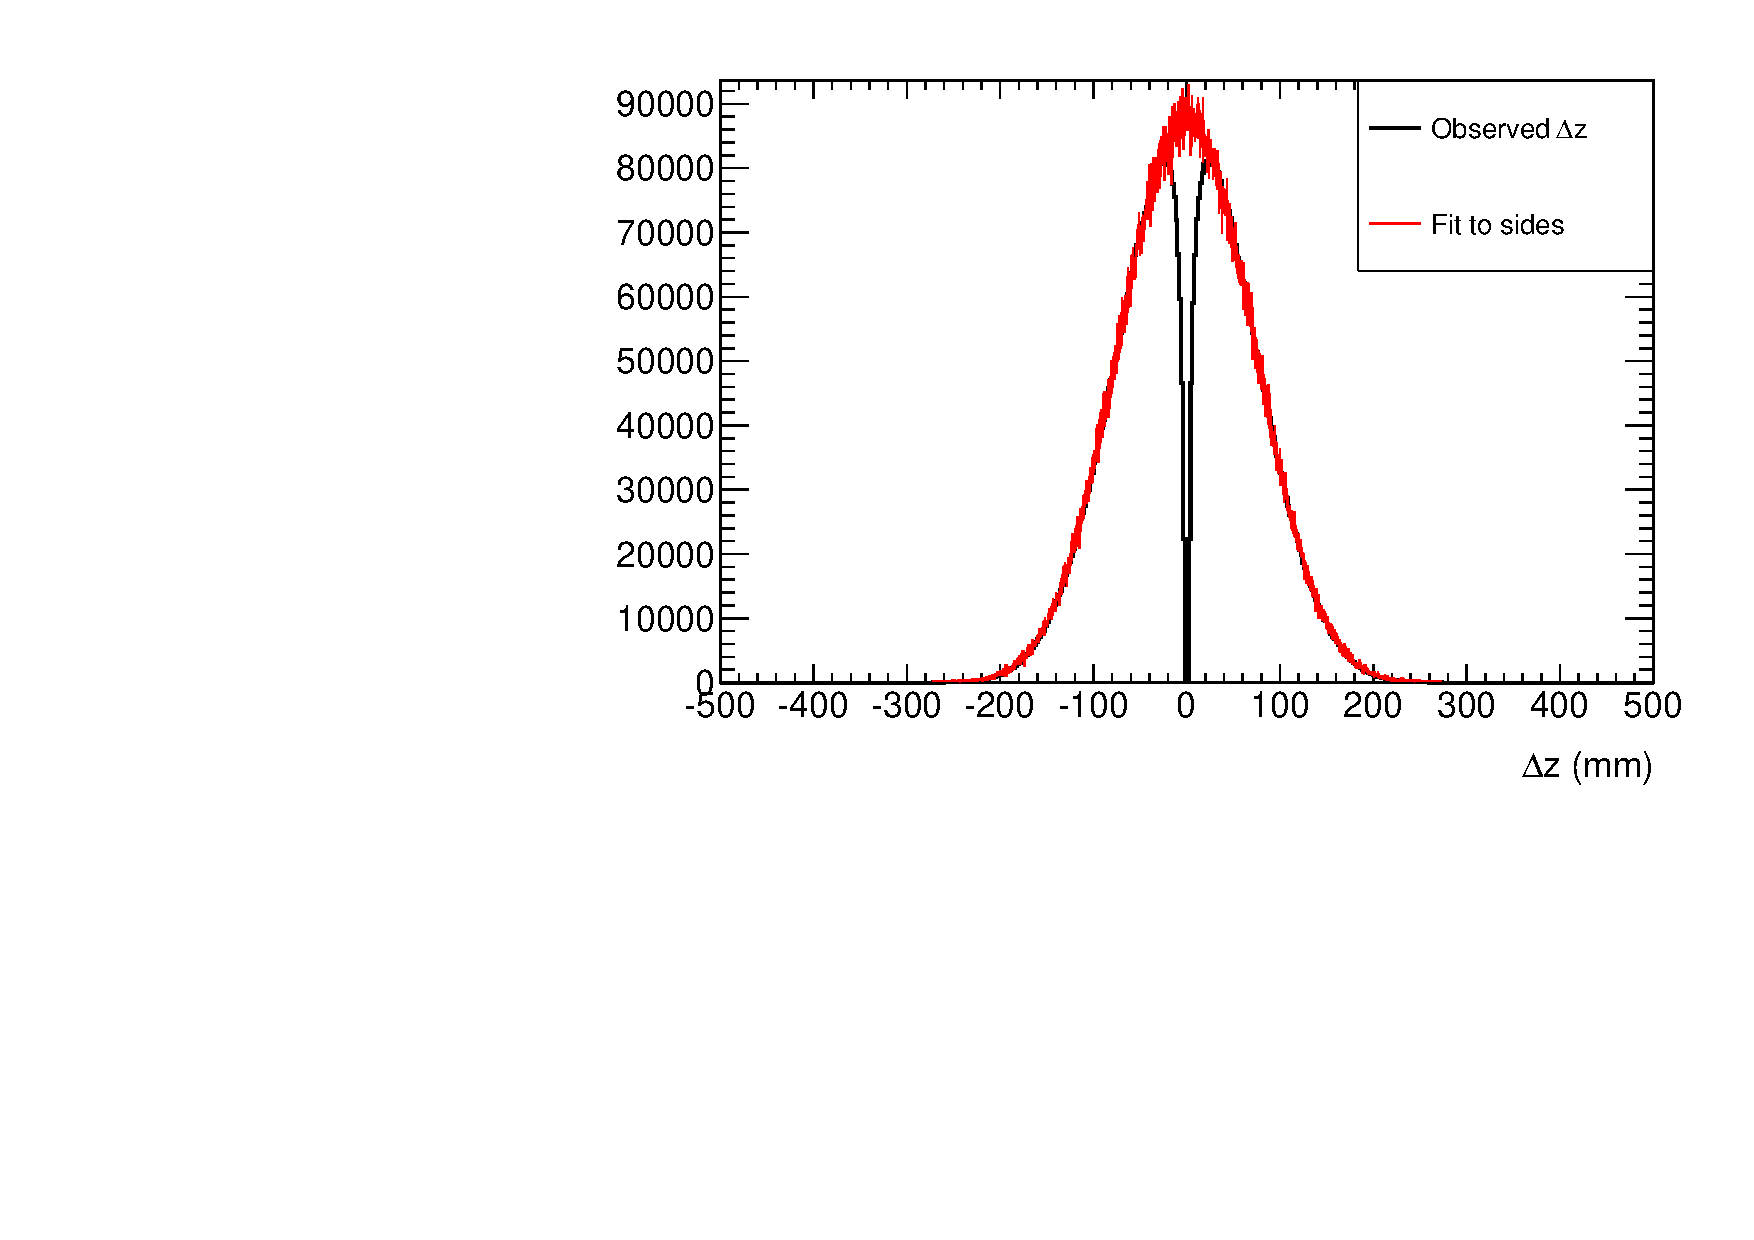
\includegraphics{figures/ch4-reconstruction/c_dz_NTrk10_BCID81}}
	}
	\subfloat[$p_{\textrm{mask}}(\Delta z)$, NTrk10] {
		\resizebox{3in}{!}{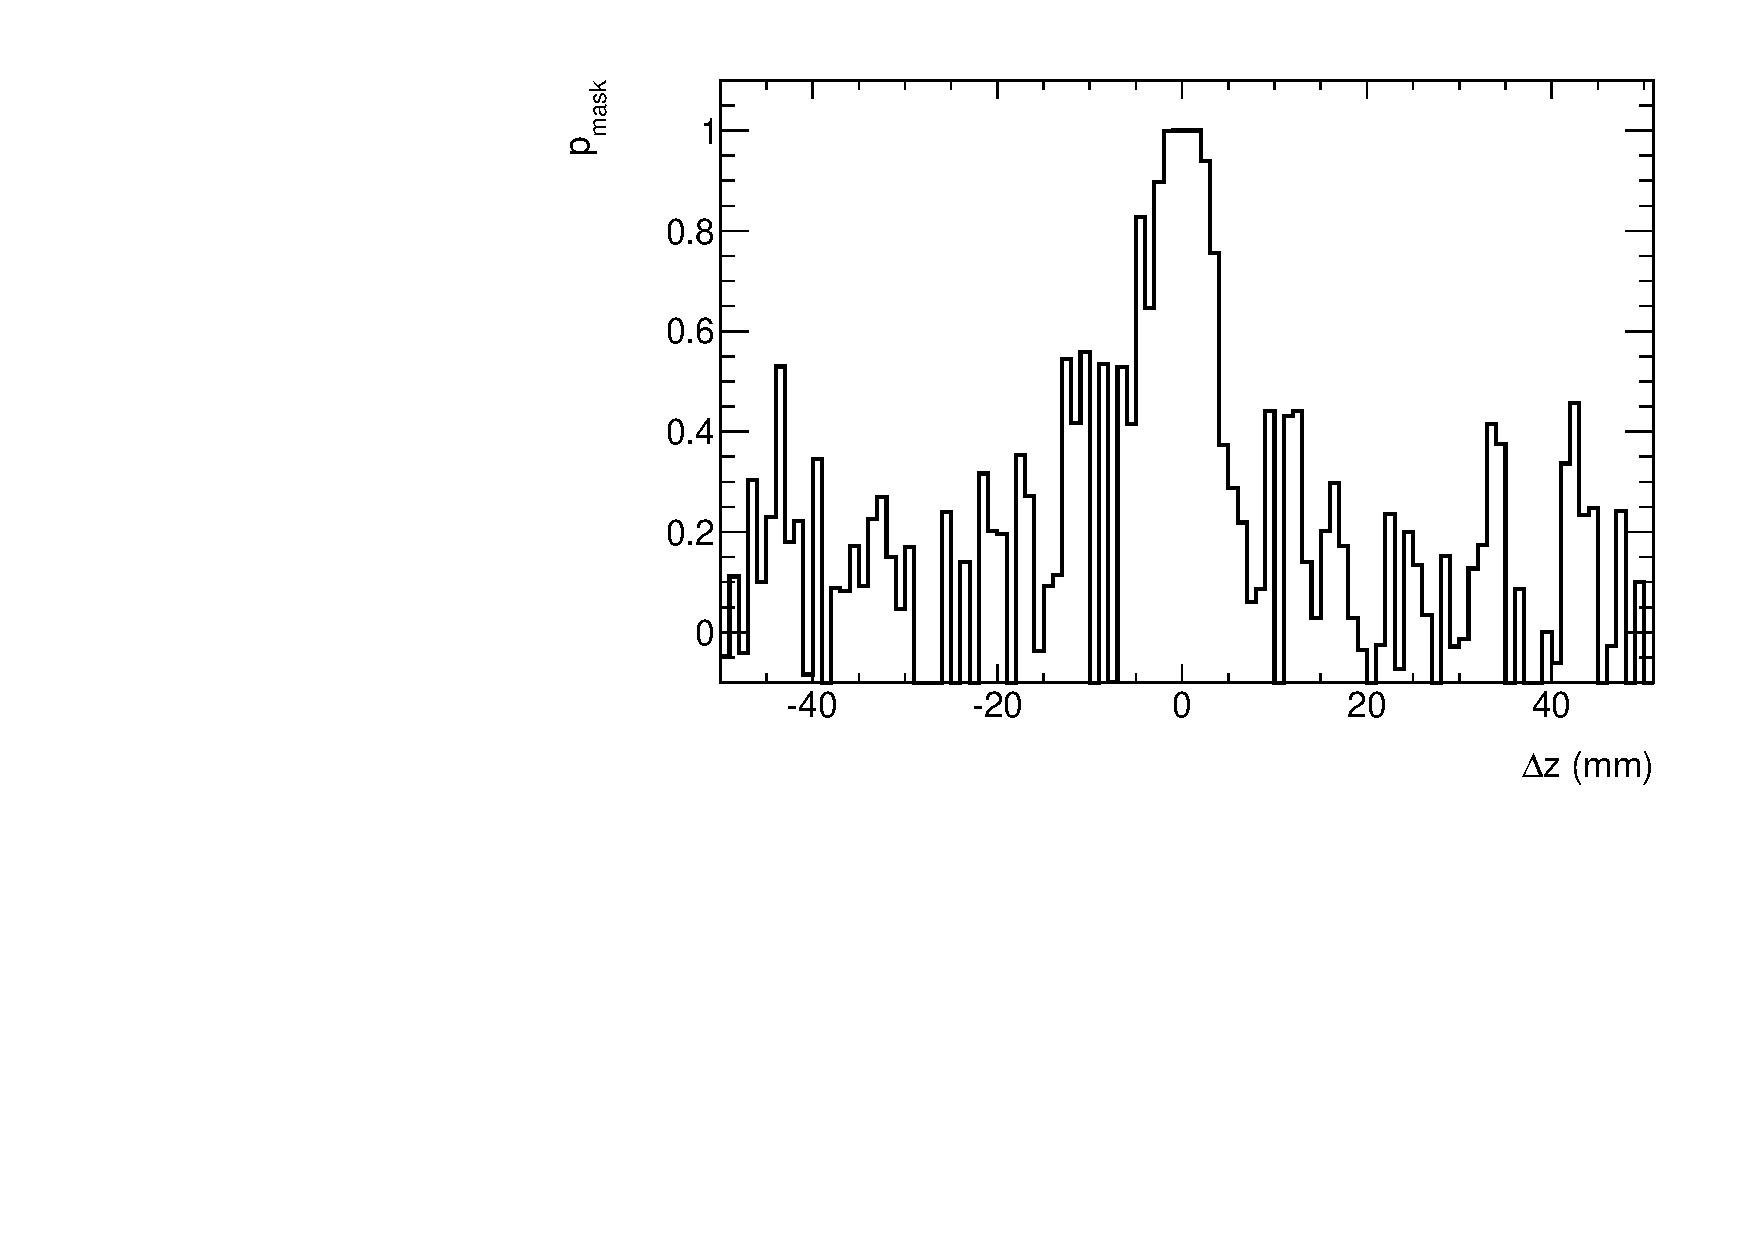
\includegraphics{figures/ch4-reconstruction/c_pmask_dz_NTrk10}}
	}\\
	\caption{Calibration of the masking correction method on data, using run 182013. Left: $\Delta z$ distributions and template fits using expected $\Delta z$ distributions in the range $30$~mm$\leq\Delta z\leq300$~mm. Right: pairwise vertex masking probability as a function of the longitudinal distance $\Delta z$ between the vertices.}
	\label{fig:masking-correction-data}
\end{figure}

\begin{figure}[p]
	\centering
	\subfloat[$\Delta z$ distribution and template fit, NTrk5] {
		\resizebox{3in}{!}{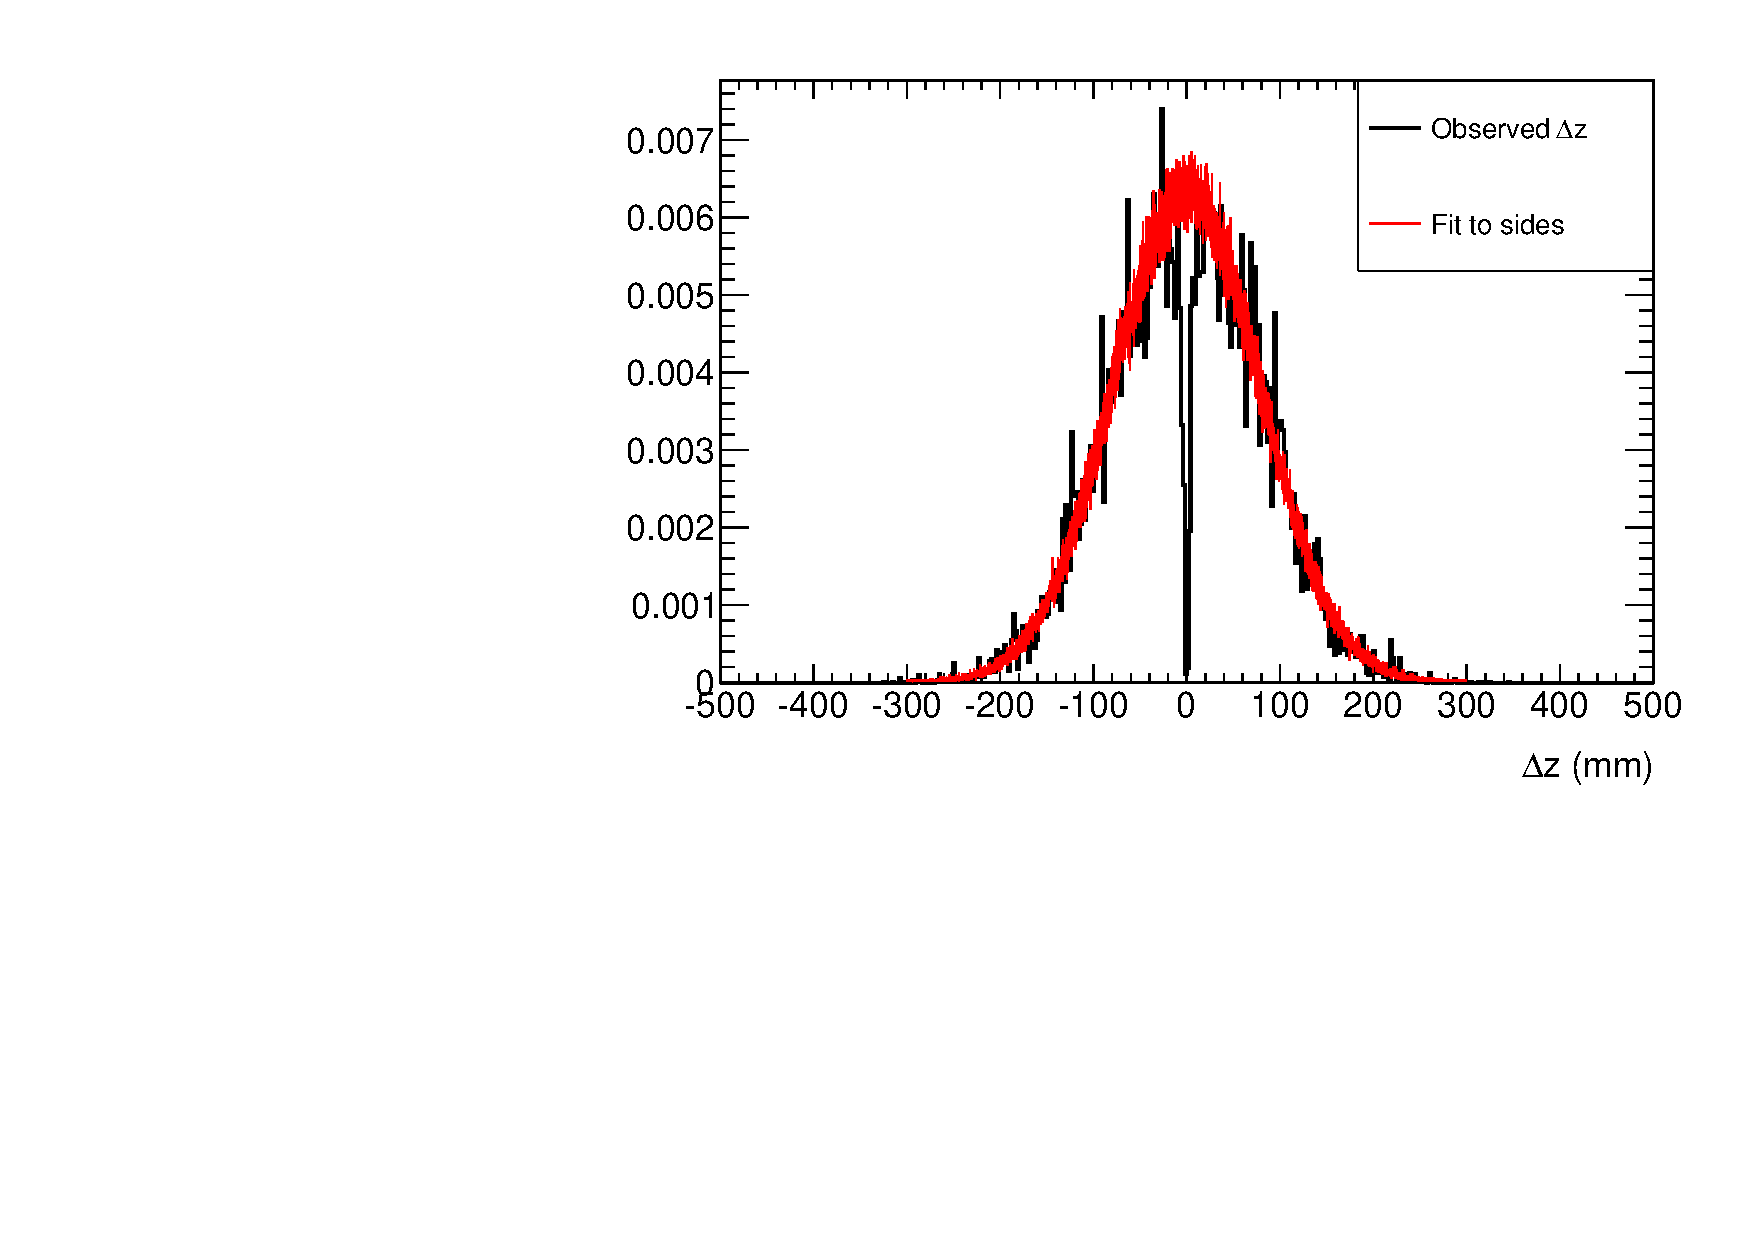
\includegraphics{figures/ch4-reconstruction/c_dz_NTrk5}}
	}
	\subfloat[$p_{\textrm{mask}}(\Delta z)$, NTrk5] {
		\resizebox{3in}{!}{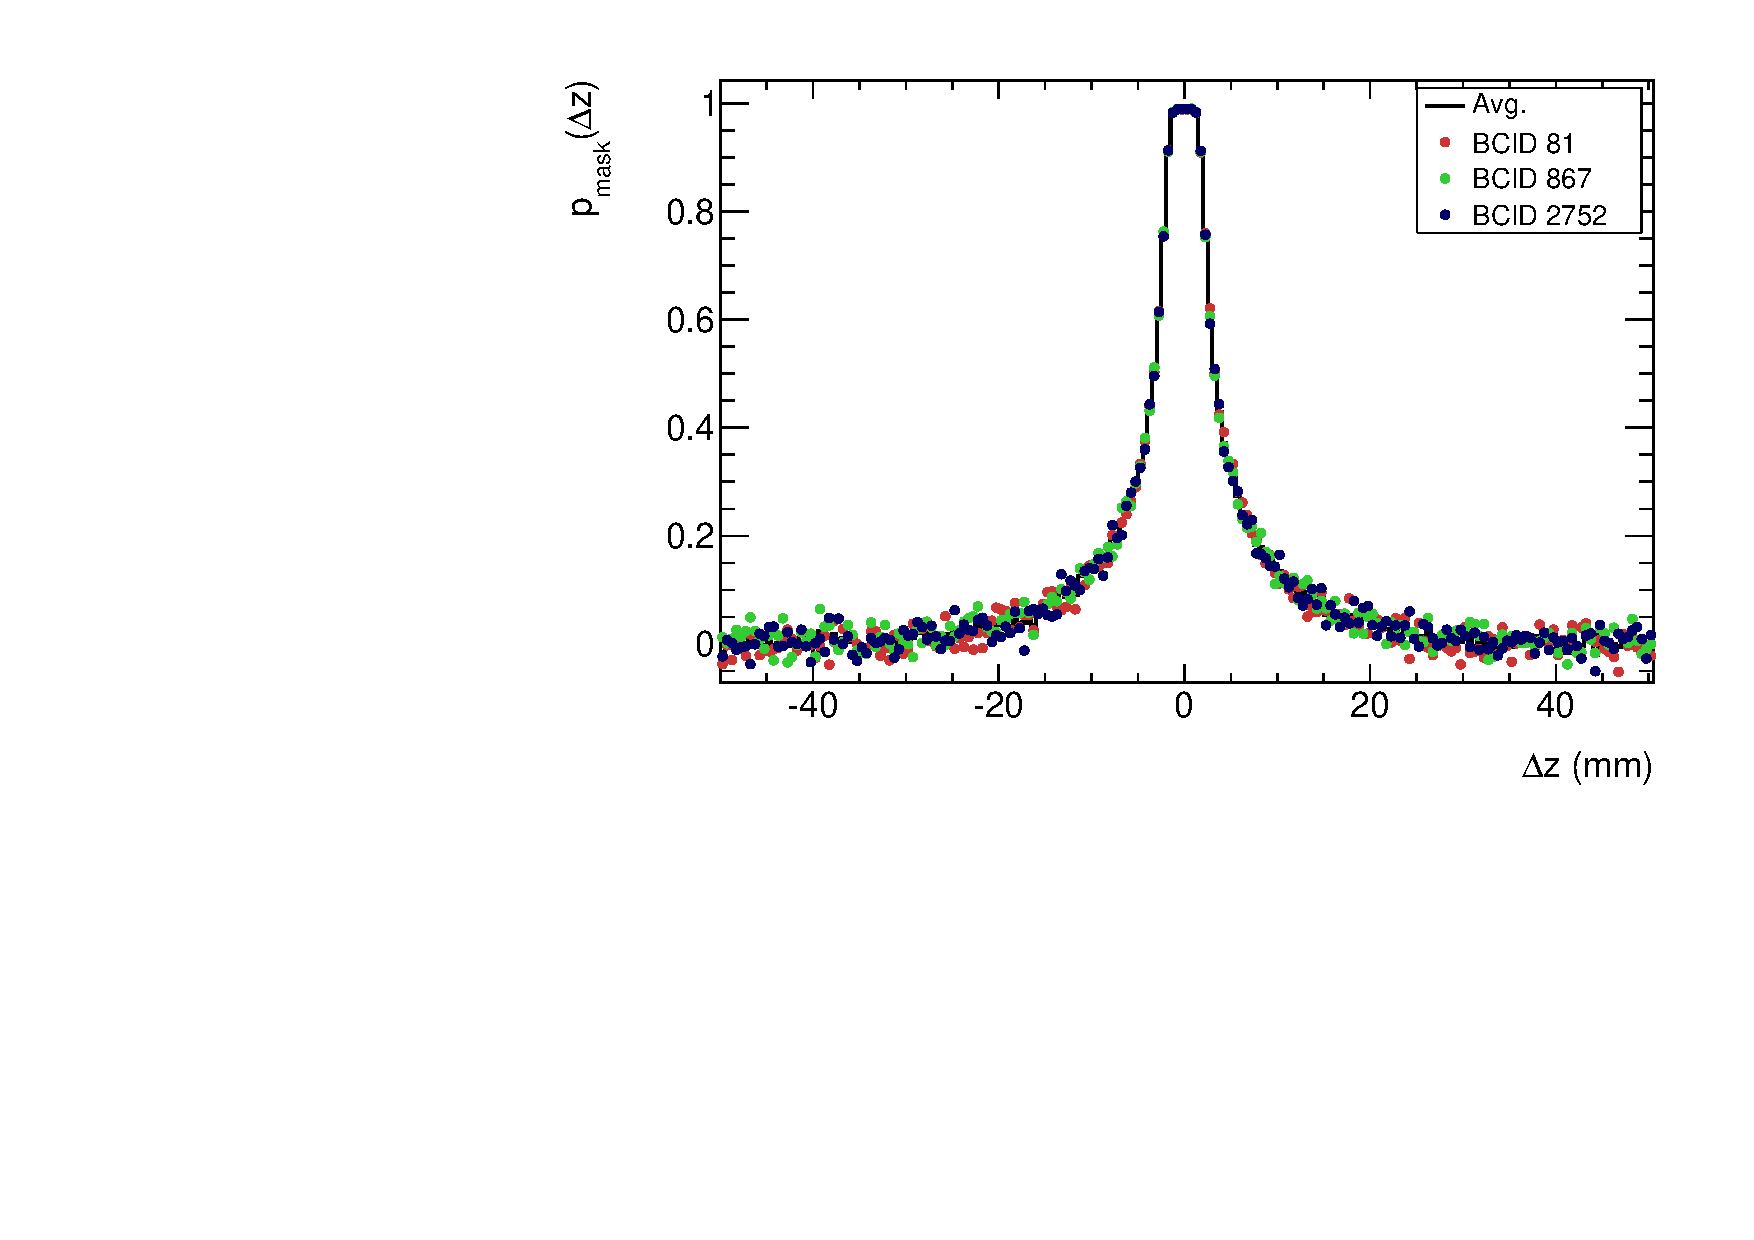
\includegraphics{figures/ch4-reconstruction/c_pmask_dz_NTrk5}}
	}\\
	\subfloat[$\Delta z$ distribution and template fit, NTrk7] {
		\resizebox{3in}{!}{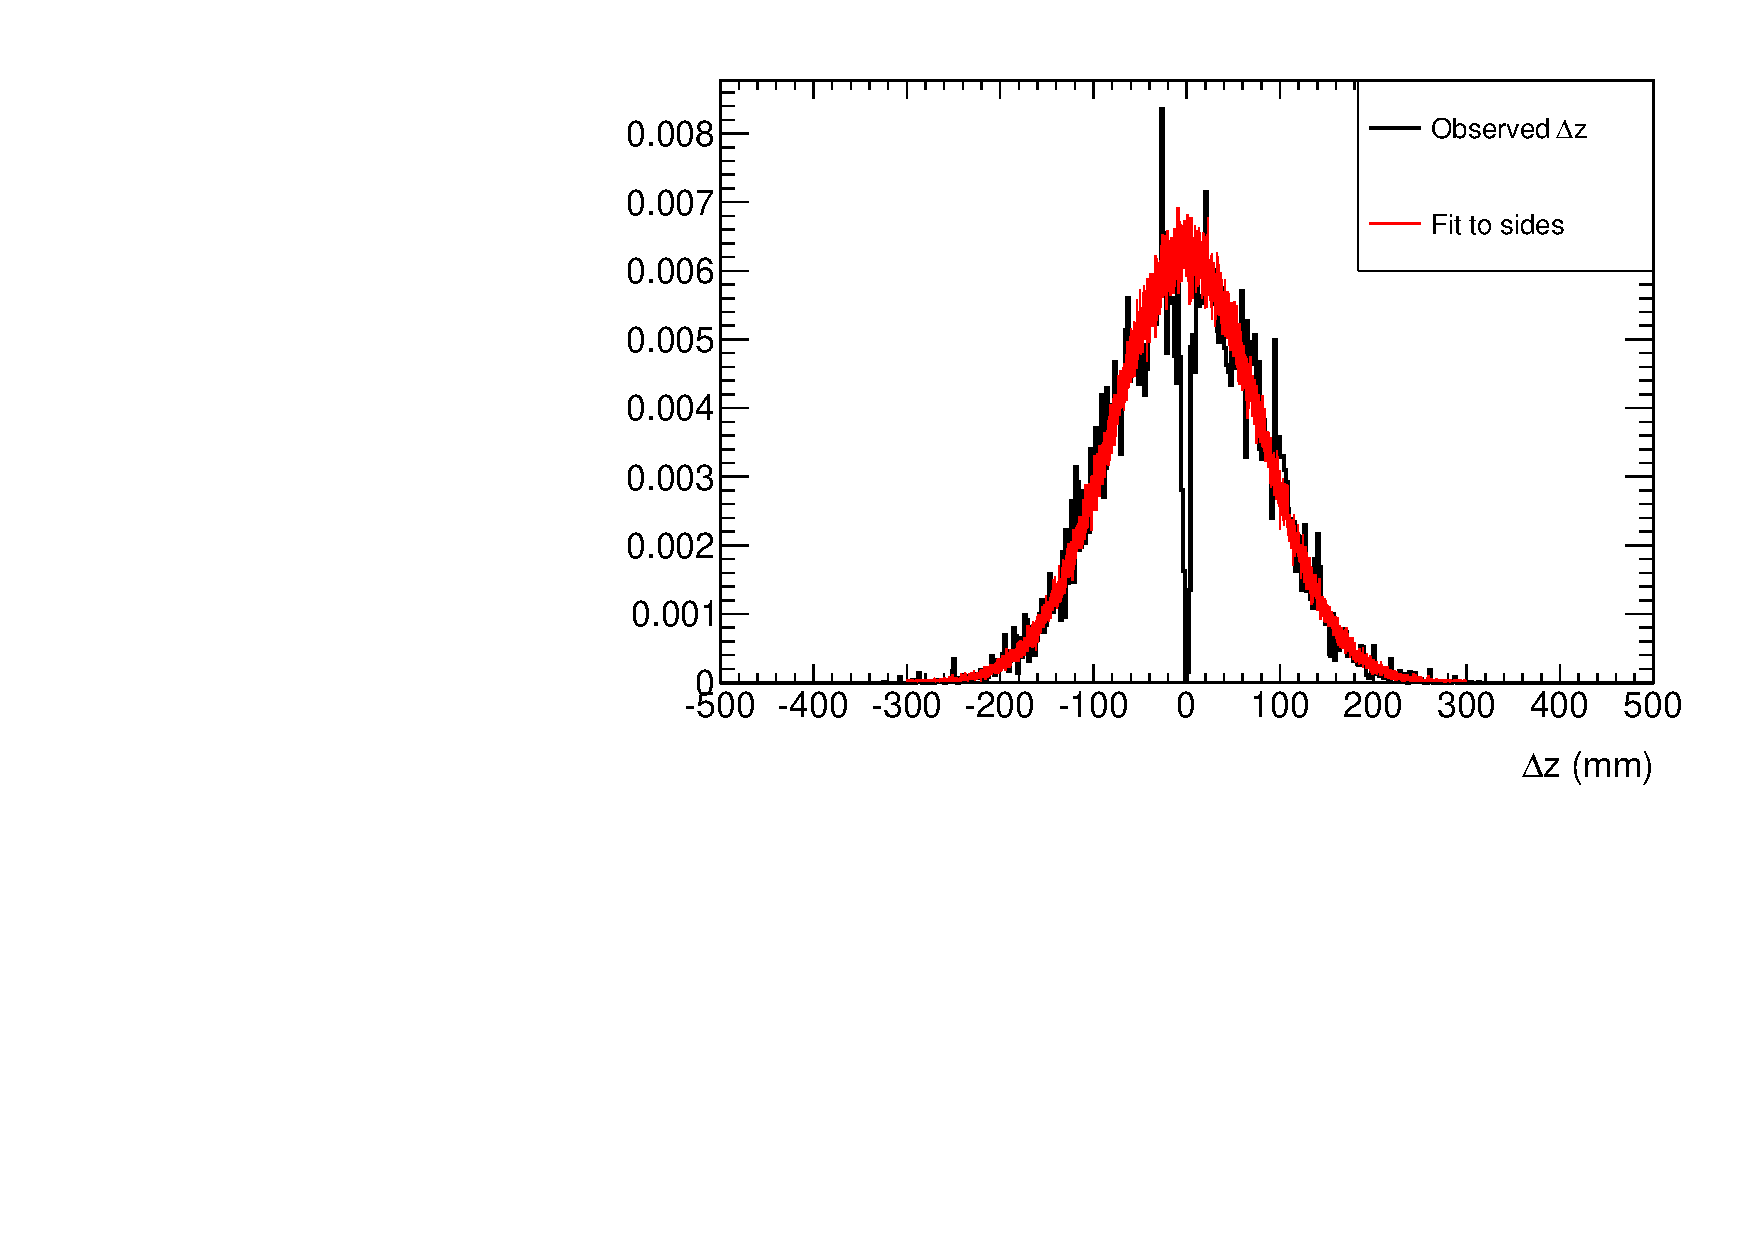
\includegraphics{figures/ch4-reconstruction/c_dz_NTrk7}}
	}
	\subfloat[$p_{\textrm{mask}}(\Delta z)$, NTrk7] {
		\resizebox{3in}{!}{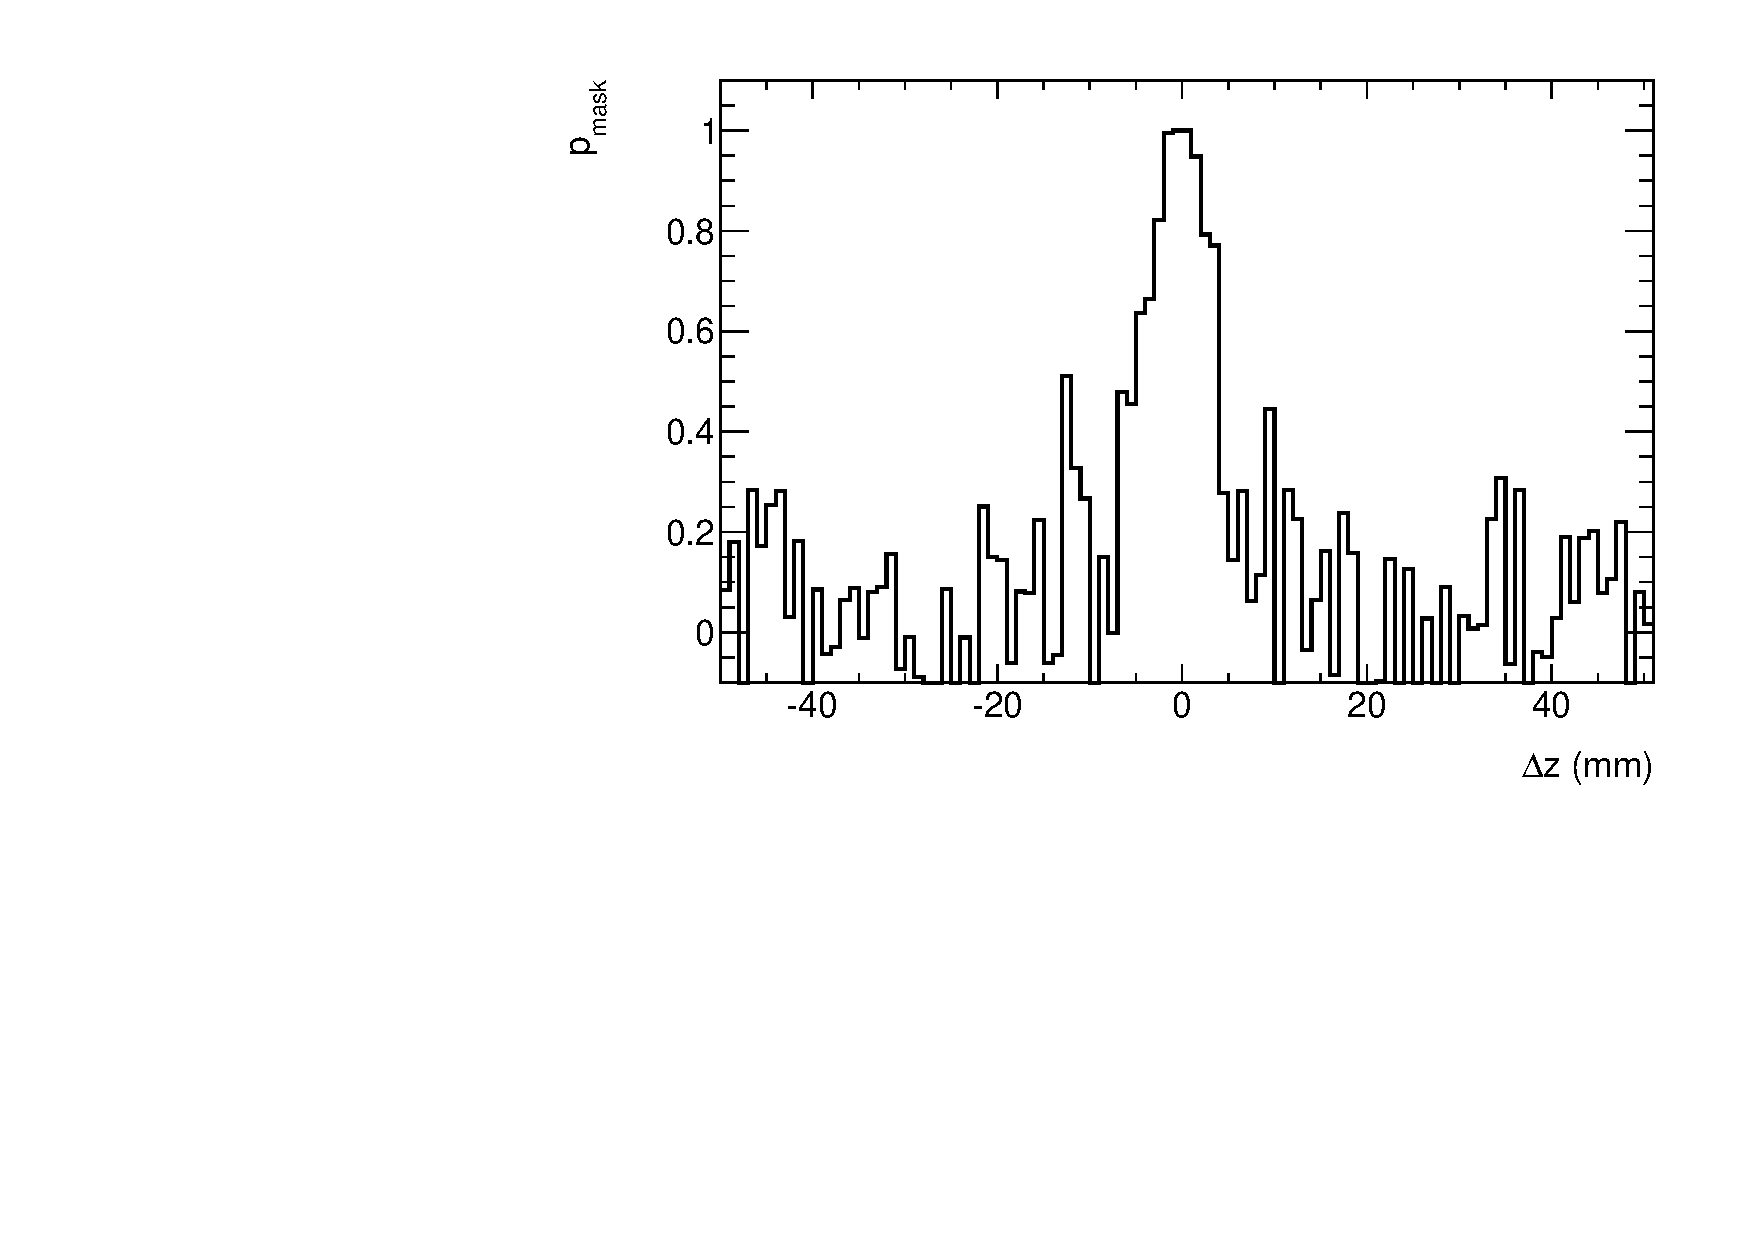
\includegraphics{figures/ch4-reconstruction/c_pmask_dz_NTrk7}}
	}\\
	\subfloat[$\Delta z$ distribution and template fit, NTrk10] {
		\resizebox{3in}{!}{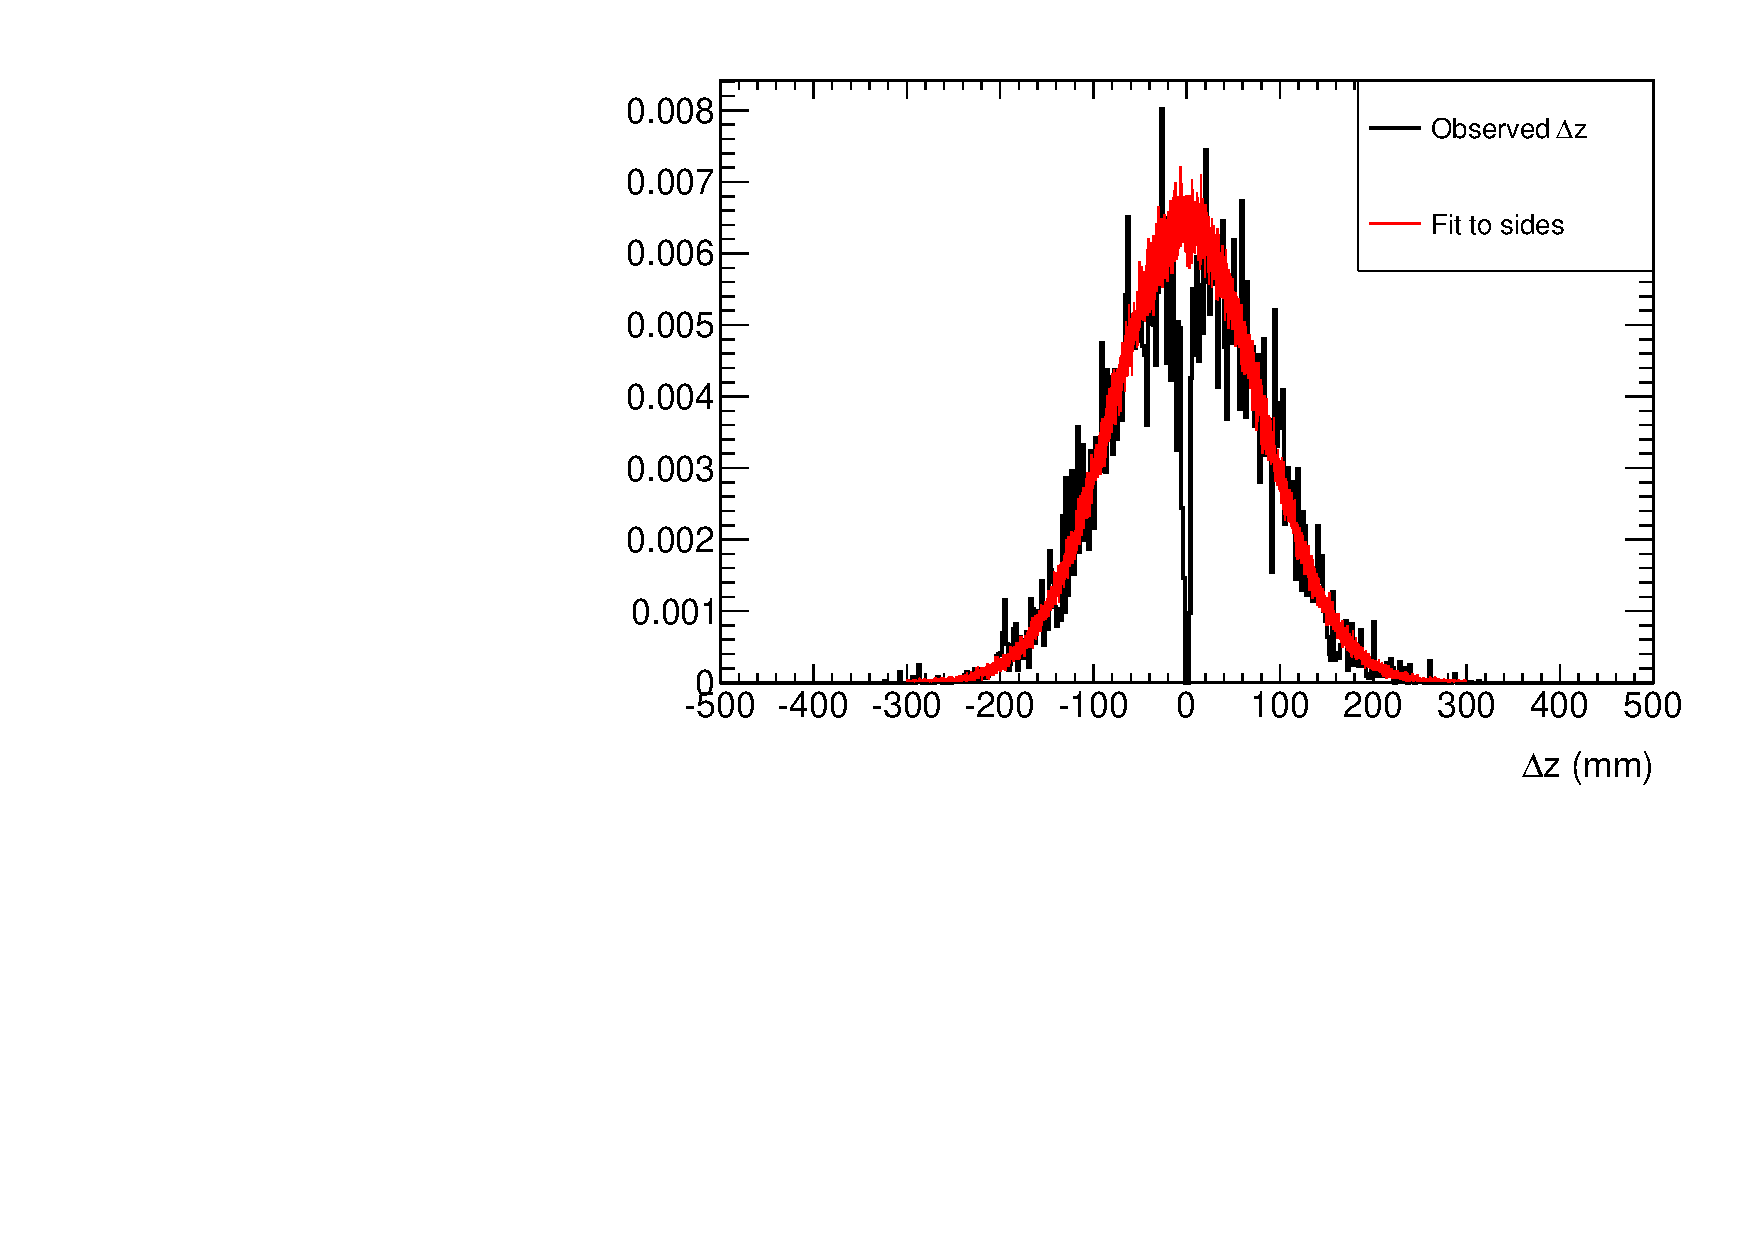
\includegraphics{figures/ch4-reconstruction/c_dz_NTrk10}}
	}
	\subfloat[$p_{\textrm{mask}}(\Delta z)$, NTrk10] {
		\resizebox{3in}{!}{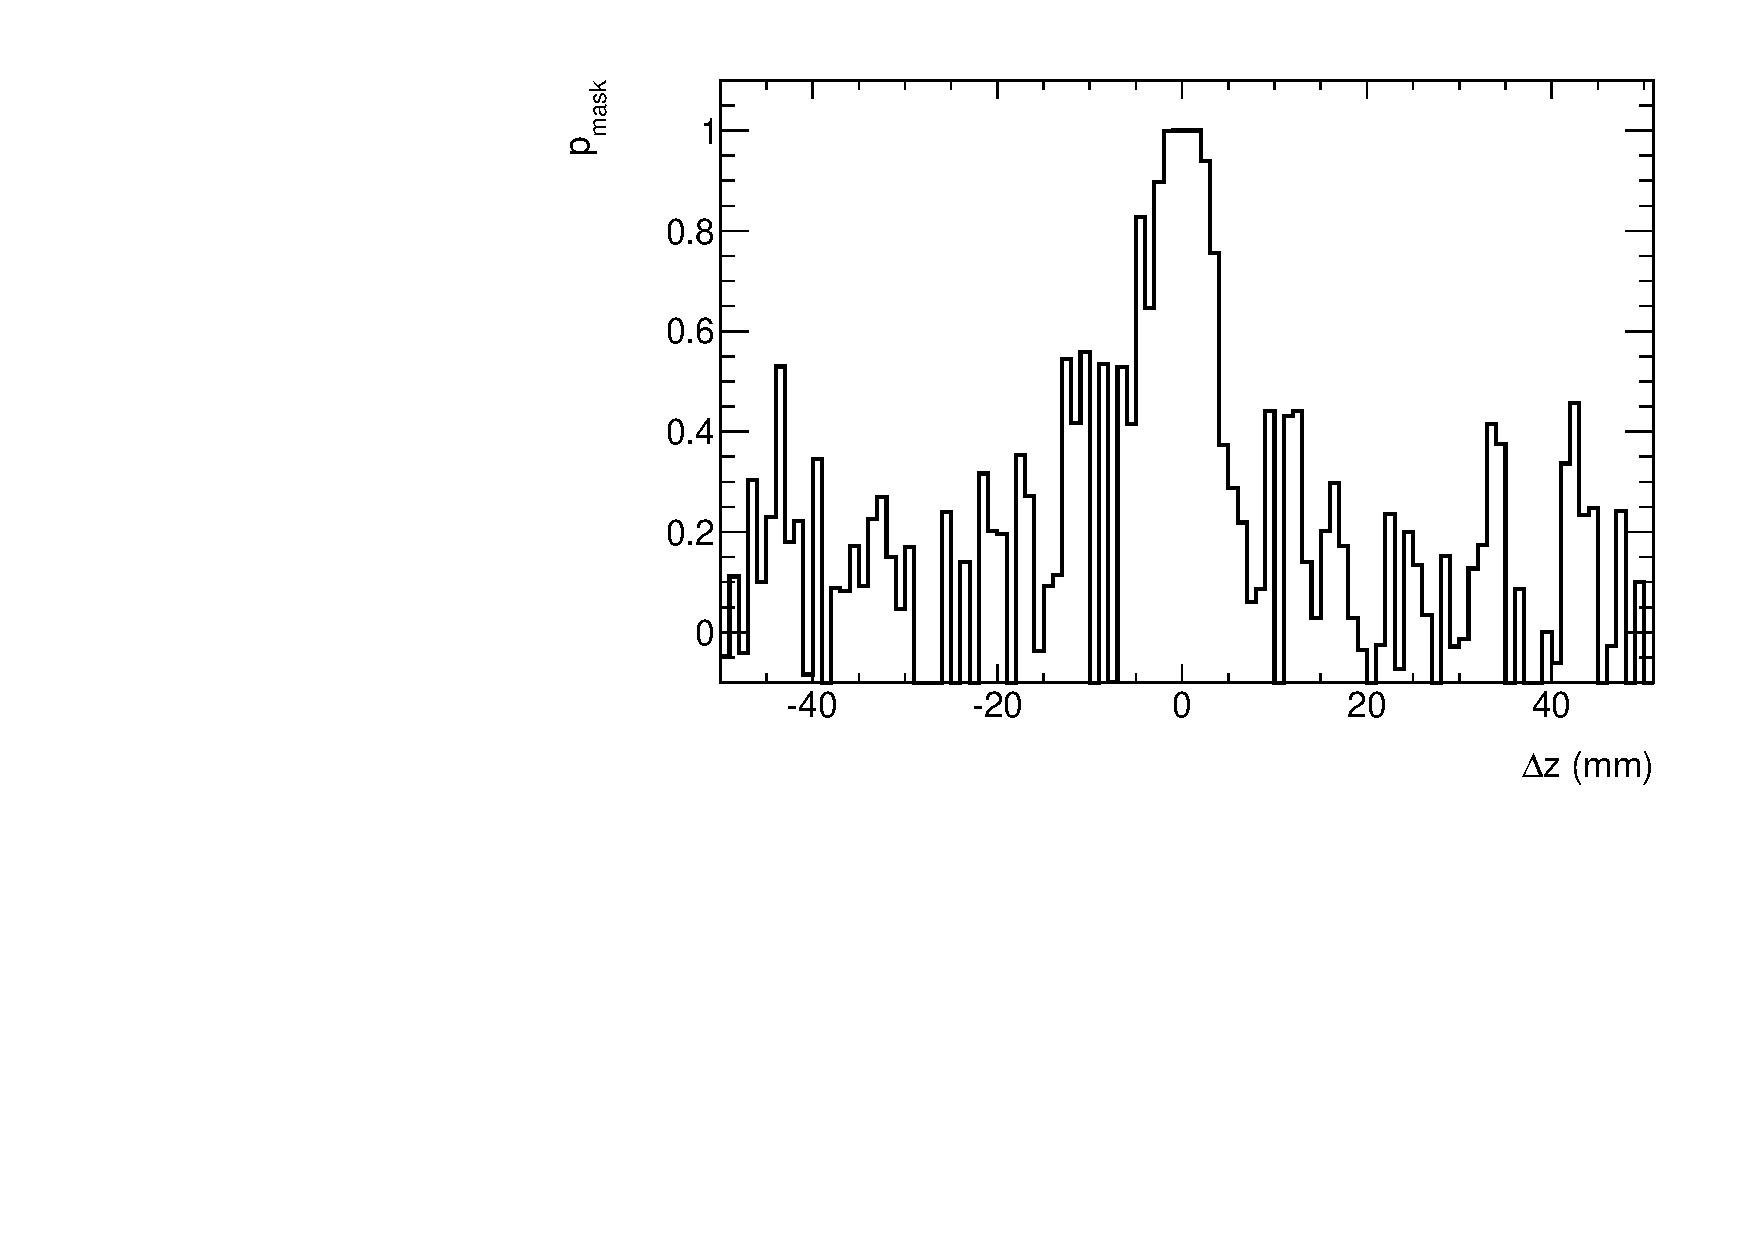
\includegraphics{figures/ch4-reconstruction/c_pmask_dz_NTrk10}}
	}\\
	\caption{Calibration of the masking correction method on simulation, using 8~TeV minimum bias Monte Carlo (pythia 8, tune A2M). Left: $\Delta z$ distributions and template fits using expected $\Delta z$ distributions in the range $30$~mm$\leq\Delta z\leq300$~mm. Right: pairwise vertex masking probability as a function of the longitudinal distance $\Delta z$ between the vertices.}
	\label{fig:masking-correction-mc}
\end{figure}

\subsubsection{Vertex-Based Luminosity Measurements}
Due to the low event rate available during physics runs, vertex counting was used to measure luminosity only in three special runs during 2011, where inner detector data was recorded by a special high-rate data stream. The data stream reads out events at $\mathcal{O}(10~\mbox{kHz}$, recording only the inner detector from a small number of bunch crossings, typically less than four. The three runs are the vdM calibration run in May 2011, the pileup scan in September 2011 shown in figure~\ref{fig:reco-luminosity-comparisons-pileup}, and a high-$\beta^{*}$ run with a single bunch used to measure the total $pp$ cross section using the ALFA detector. 

\ 

\textbf{Van der Meer Scan}

An example scan curve from the May 2011 vdM scan is shown in figure~\ref{fig:reco-luminosity-vertex-vdm}. The trigger used to collect the data requires hits in the minimum bias trigger scintillators (MBTS), and selects 3 of the 14 colliding bunch pairs. The peak interaction rate during the scan is $\mu\sim1.97$. The data are corrected for vertex masking and fakes, with the correction factor reaching up to 3\% at the peak of the scan curves. Following the protocol described in section~\ref{sec:reco-luminosity-calibration}, the visible cross section is determined to be $38.6\pm 0.14~\mbox{mb}$, where the uncertainty reflects the RMS spread between the three bunch crossings and the two scans.

\begin{figure}[p]
	\centering
	\subfloat[$x$ scan, BCID 81] {
		\resizebox{3in}{!}{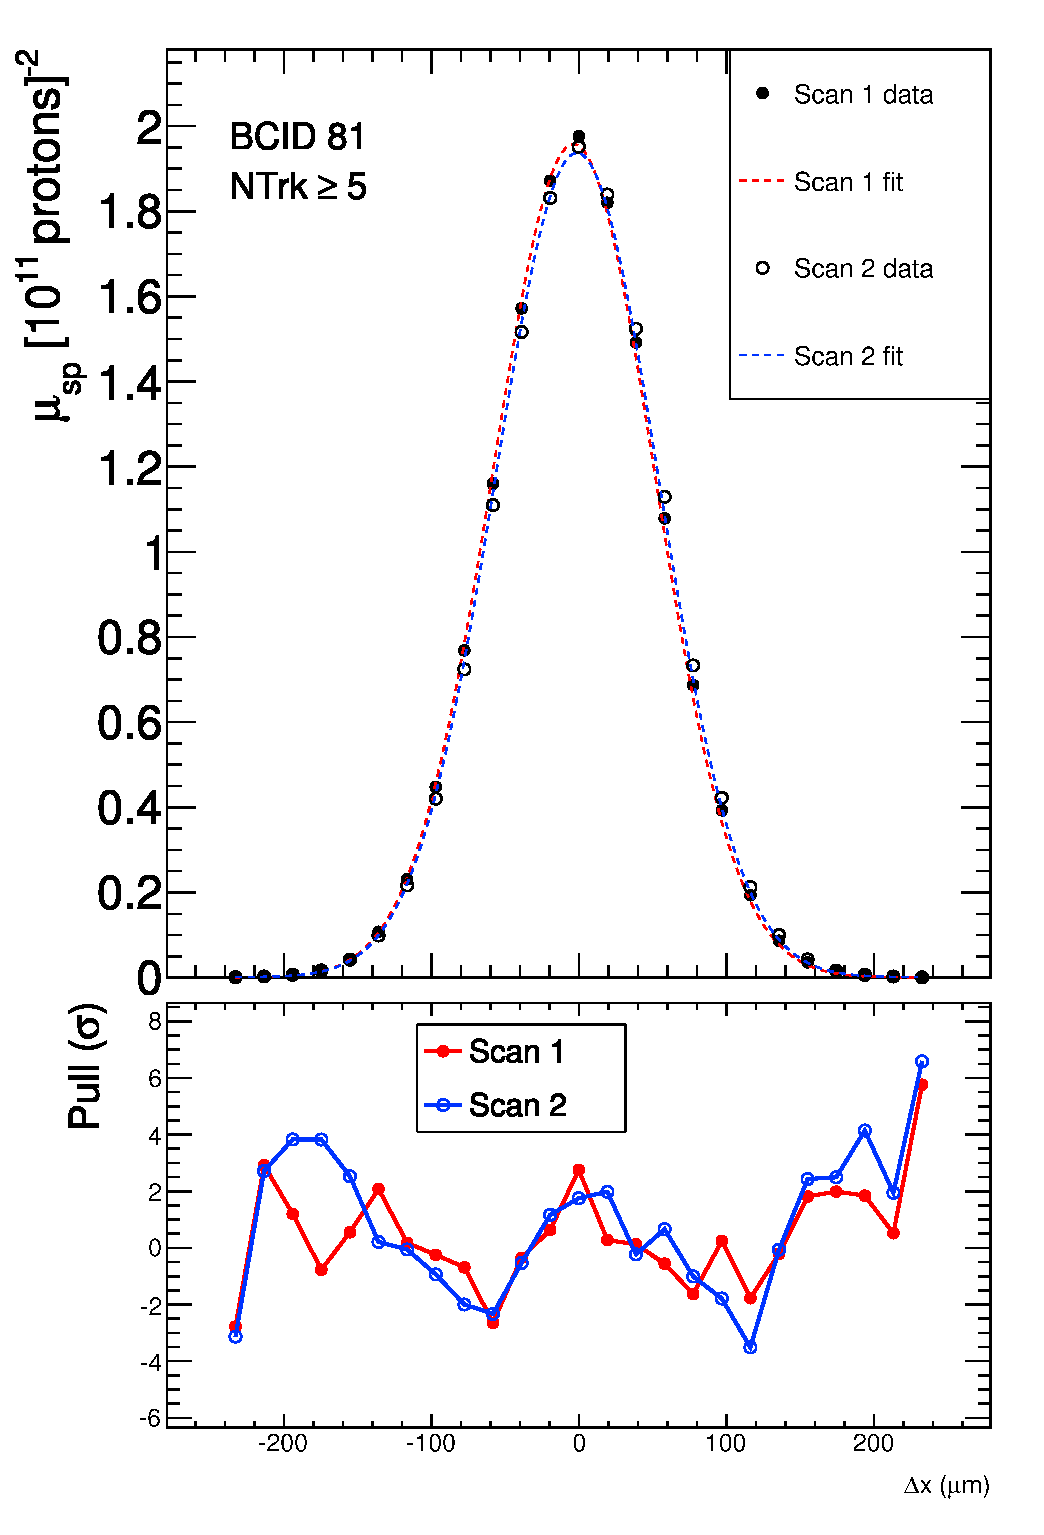
\includegraphics{figures/ch4-reconstruction/c_musp_x_BCID81_NTrkCut5}}
	}
	\subfloat[$y$ scan, BCID 81] {
		\resizebox{3in}{!}{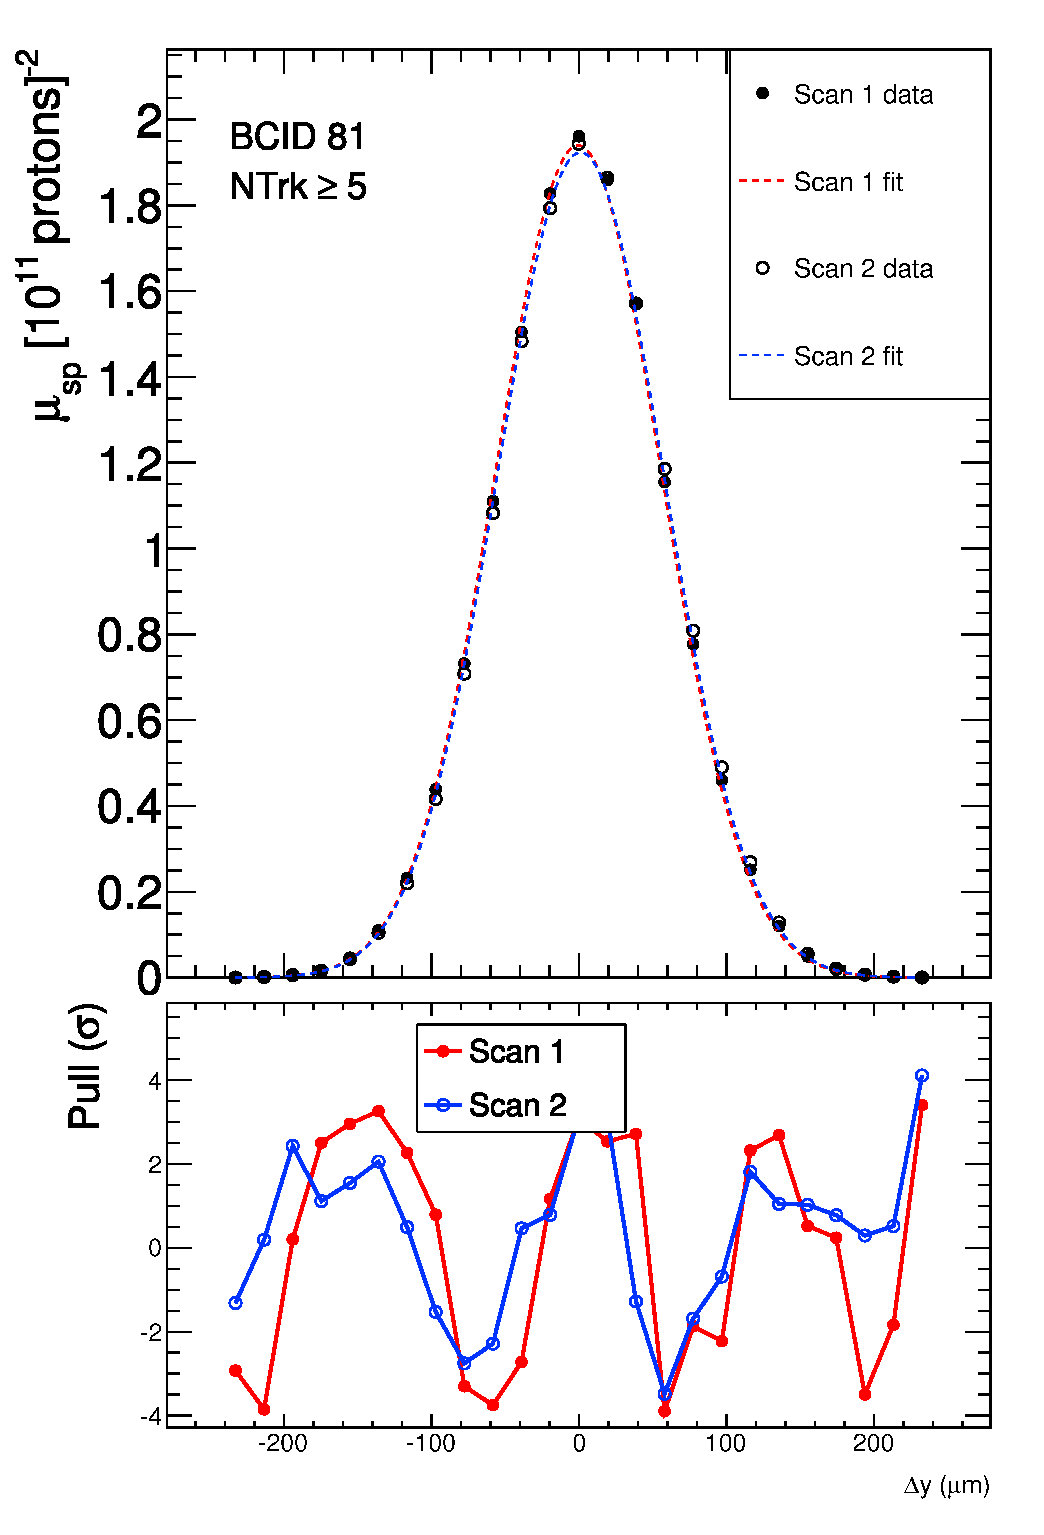
\includegraphics{figures/ch4-reconstruction/c_musp_y_BCID81_NTrkCut5}}
	}\\
	\caption{$\mu_{\textrm{vis}}^{(sp)}$ vs. beam separation, with single gaussian plus constant fits, and pulls.}
	\label{fig:reco-luminosity-vertex-vdm}
\end{figure}

\ 

\textbf{Pileup Scan}

The September 2011 pileup scan is used to derive systematic uncertainties due to the nonlinear response of algorithms with respect to the number of interactions per bunch crossing. The scan was performed at the end of a physics run, displacing the beams in the transverse direction to obtain a sample of data at different pileup values with otherwise identical conditions. The data was triggered by a random trigger selecting events from two bunch crossings, BCIDs 200 and 999. The data are corrected for vertex masking and fakes, with the correction reaching up to 10\% as shown in figure~\ref{reco-luminosity-vertexing-muscan-corrections} with respect to BCM\_VOR. A comparison of the luminosity measurements between vertex counting and BCM\_VOR, shown in figure~\ref{fig:reco-luminosity-vertexing-muscan}, exhibits a slope of about 0.1\% per unit of $\mu$.

\begin{figure}[h]
	\centering
	\subfloat[BCID 200] {
		\resizebox{6.5in}{!}{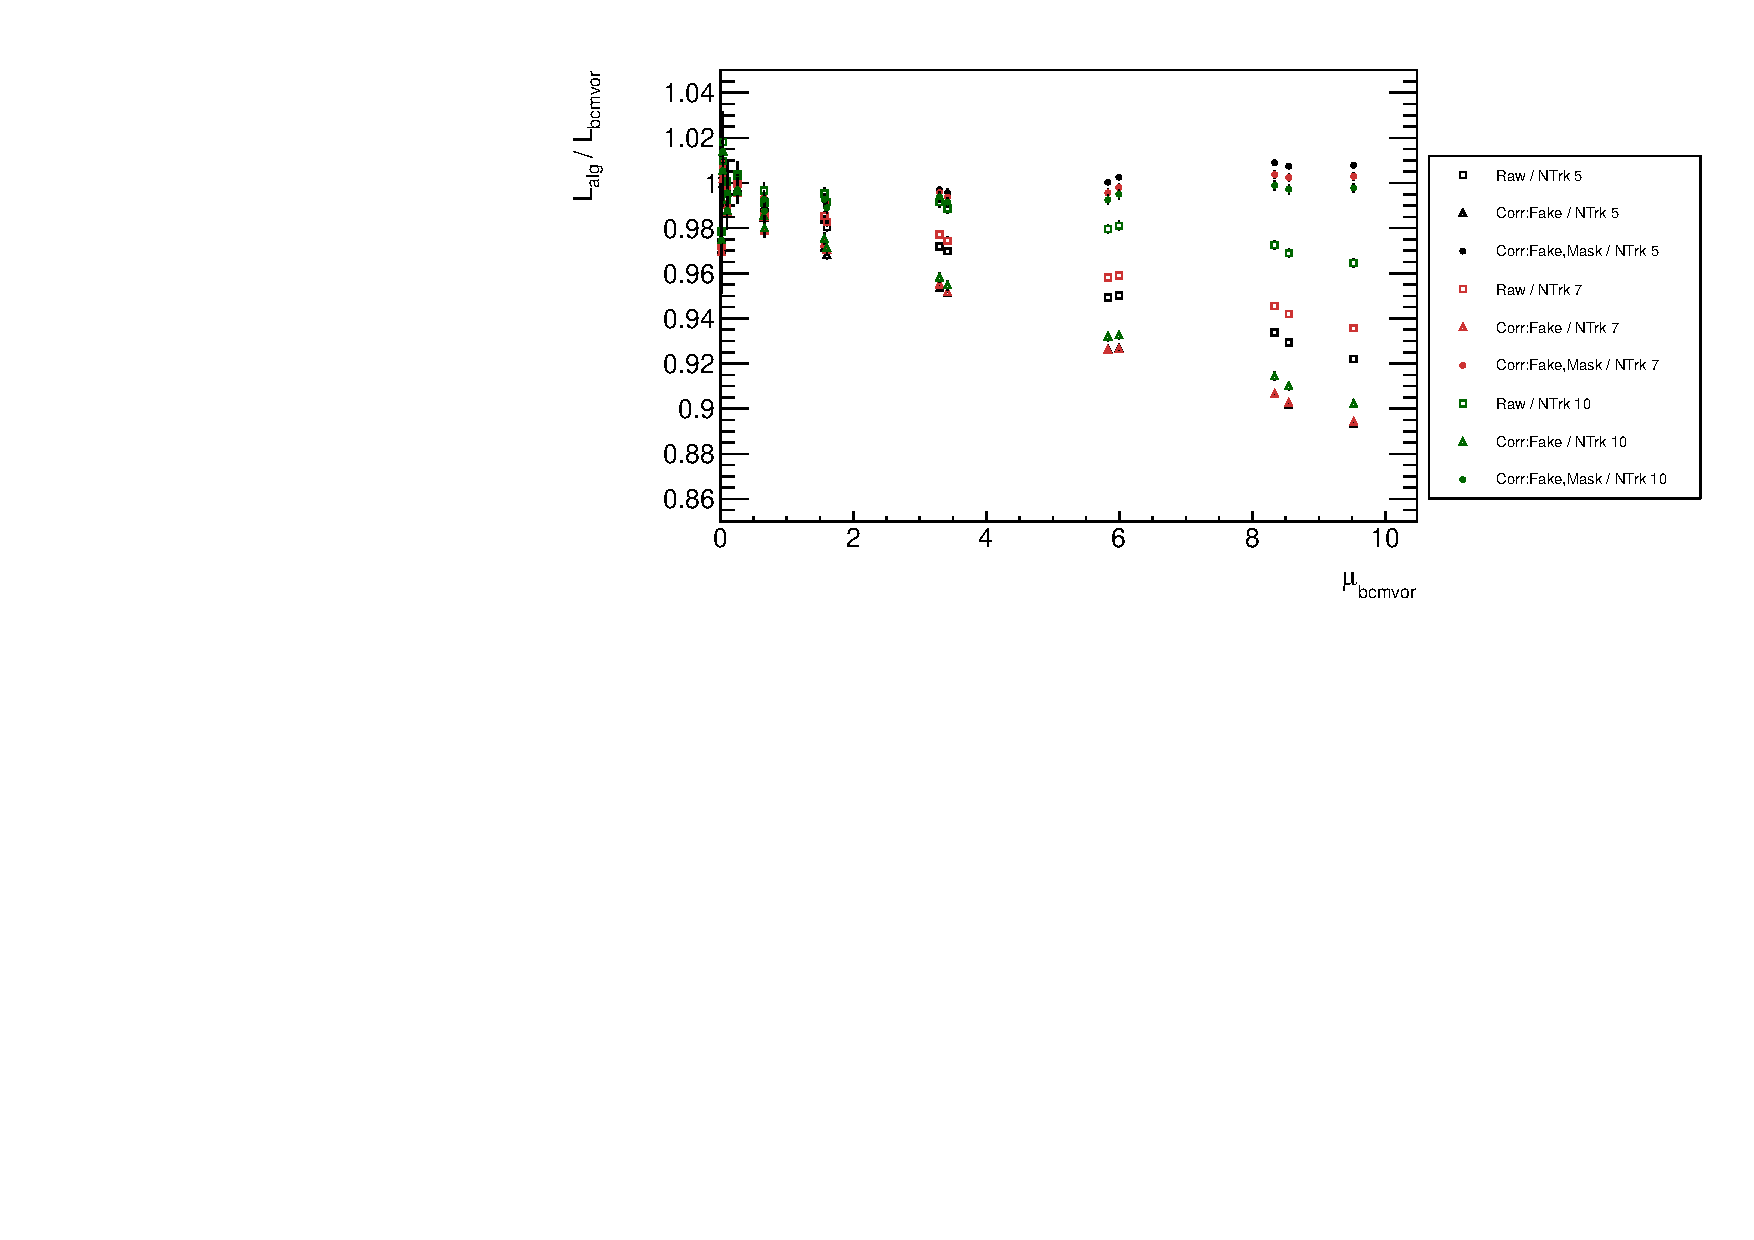
\includegraphics{figures/ch4-reconstruction/c_pileup_corrections_NVtx_BCID200}}
	}\\
	\subfloat[BCID 999] {
		\resizebox{6.5in}{!}{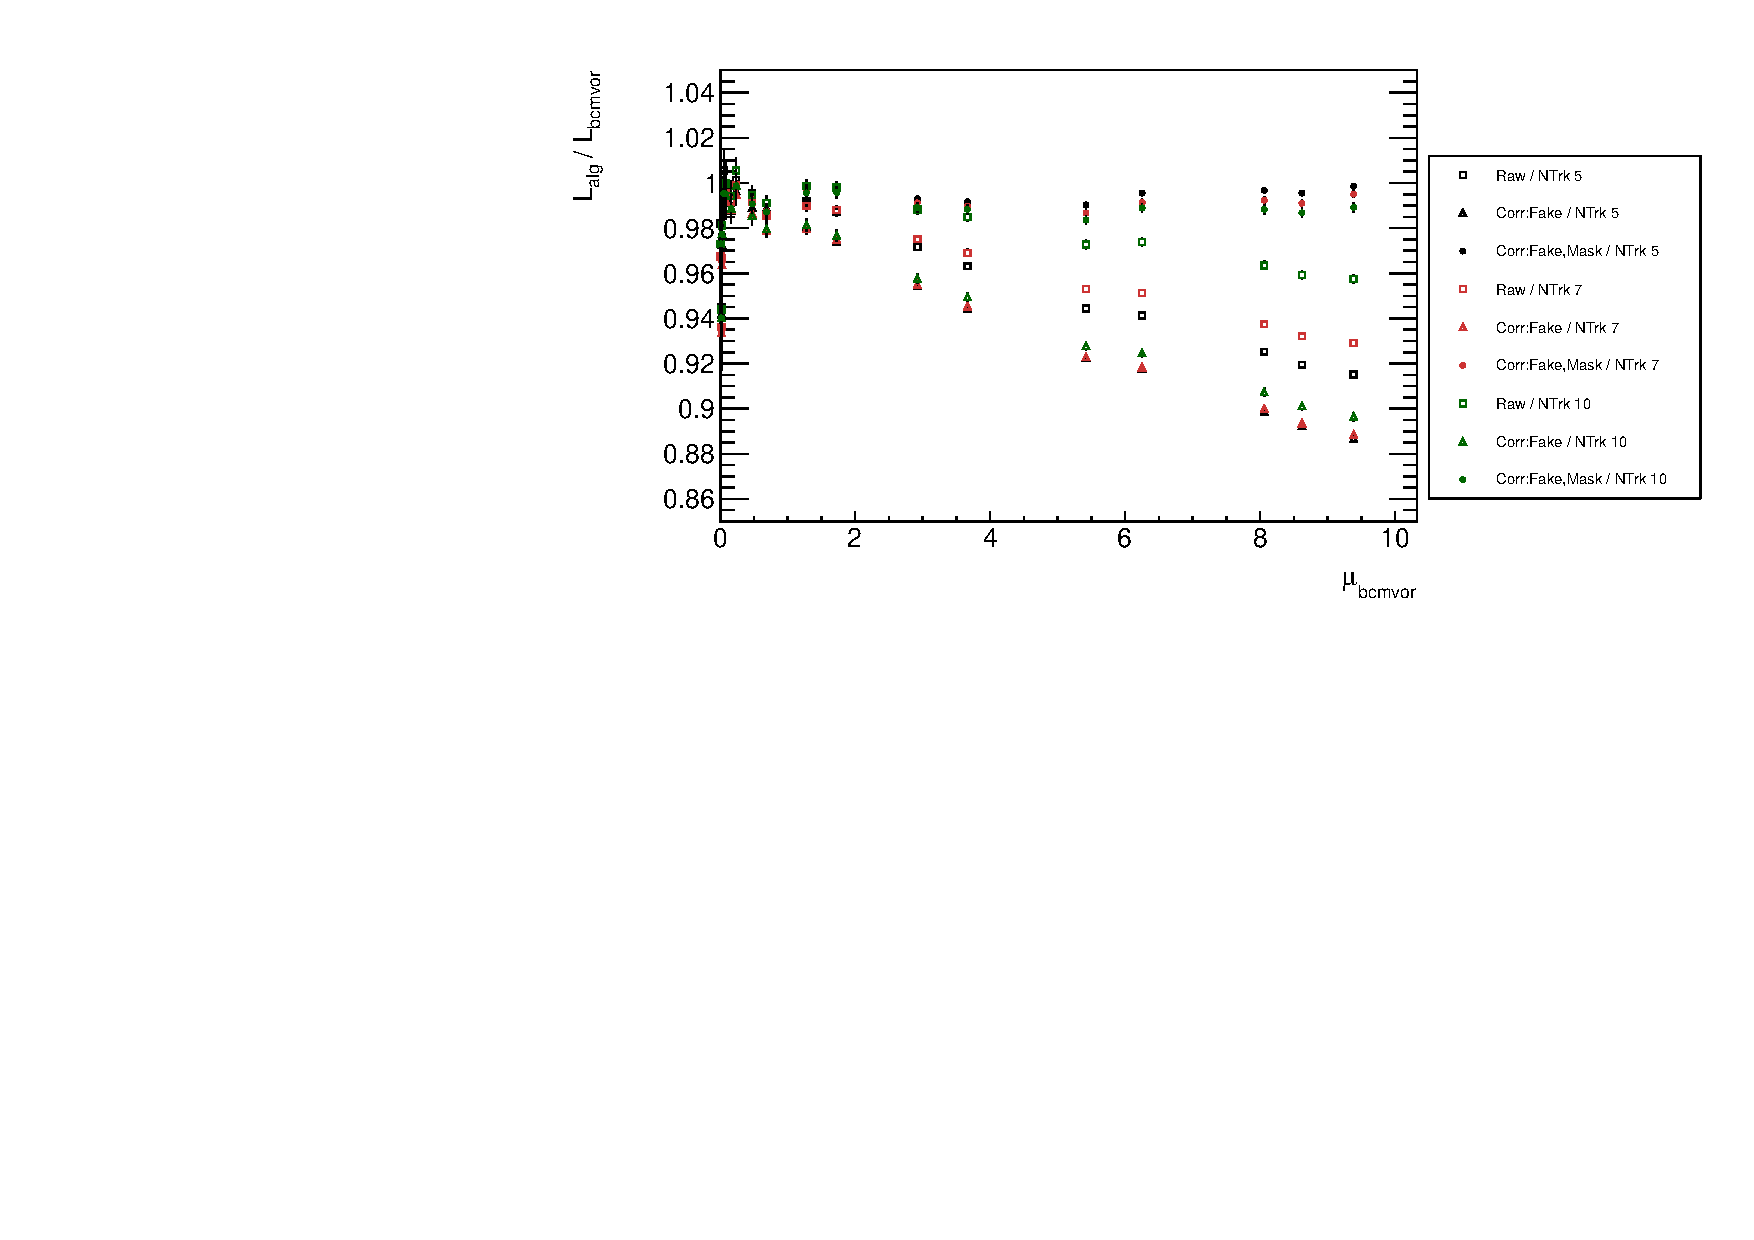
\includegraphics{figures/ch4-reconstruction/c_pileup_corrections_NVtx_BCID999}}
	}
	\caption{Ratio of luminosity values from vertexing and BCM\_VOR, shown with each successive pileup correction applied. Fakes are subtracted first, and masking is corrected second.}
	\label{reco-luminosity-vertexing-muscan-corrections}
\end{figure}

\begin{figure}[h]
	\centering
	\resizebox{6in}{!}{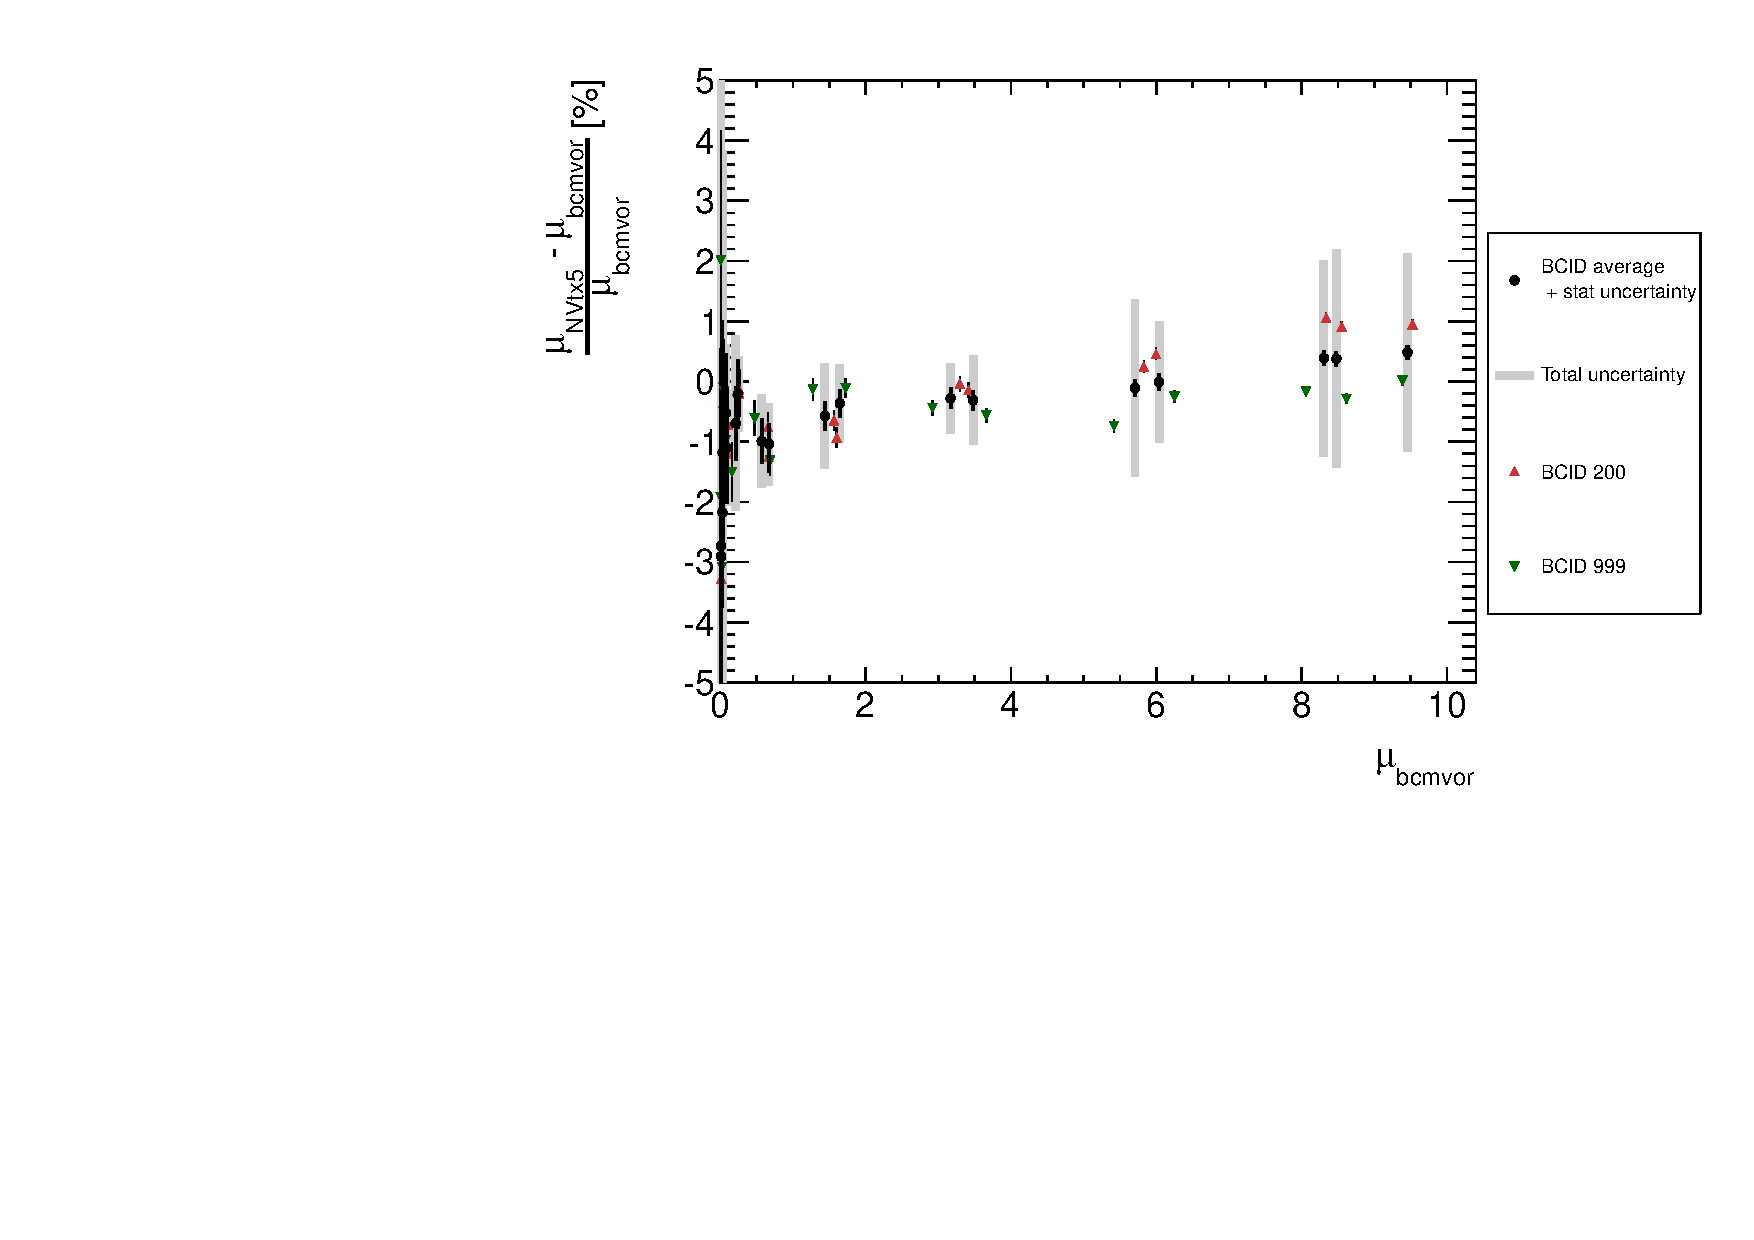
\includegraphics{figures/ch4-reconstruction/c_muscan}}
	\caption{Percent difference between luminosities measured by vertex counting and BCM\_VOR. The central values are taken to be the average between BCIDs 200 and 999.}
	\label{fig:reco-luminosity-vertexing-muscan}
\end{figure}

\ 

\textbf{ALFA Run}

Finally, vertex counting provides a reliable luminosity measurement for the 2011 ALFA run, a special run used for a measurement of the total $pp$ cross section. The beams contain a single colliding bunch pair with $\beta^{*}=90~\mbox{m}$ and $\mu\sim0.03$, in order to measure the scattering angle of elastic $pp$ collisions. A special luminosity analysis is performed to address the very low instantaneous luminosity of $\mathcal{L}\sim5\times 10^{27} \cm^{-2}\mbox{s}^{-1}$, about six orders of magnitude lower than a typical physics fill. The calorimeter methods are unusable due to a lack of sensitivity. For BCM and LUCID, the backgrounds at low instantaneous luminosity have a different composition: afterglow is negligible with a single colliding bunch, but beam-gas interactions can be significant, resulting in an extra 0.2\% systematic uncertainty. The low-pileup conditions are ideal for vertex counting, eliminating the need to perform pileup corrections. The cut on the minimum number of tracks per vertex suppresses the beam-gas backgrounds. The data were recorded by a random trigger at approximately 1~kHz. 

A comparison of luminosity measurements from BCM, LUCID, and vertex counting is shown in figure~\ref{fig:reco-luminosity-alfa}. To be consistent with the primary $pp$ luminosity measurement, the central value is taken from BCM\_VOR; vertex counting shows agreement with this value to within $0.5\%$.

\begin{figure}[h]
	\centering
	\resizebox{5in}{!}{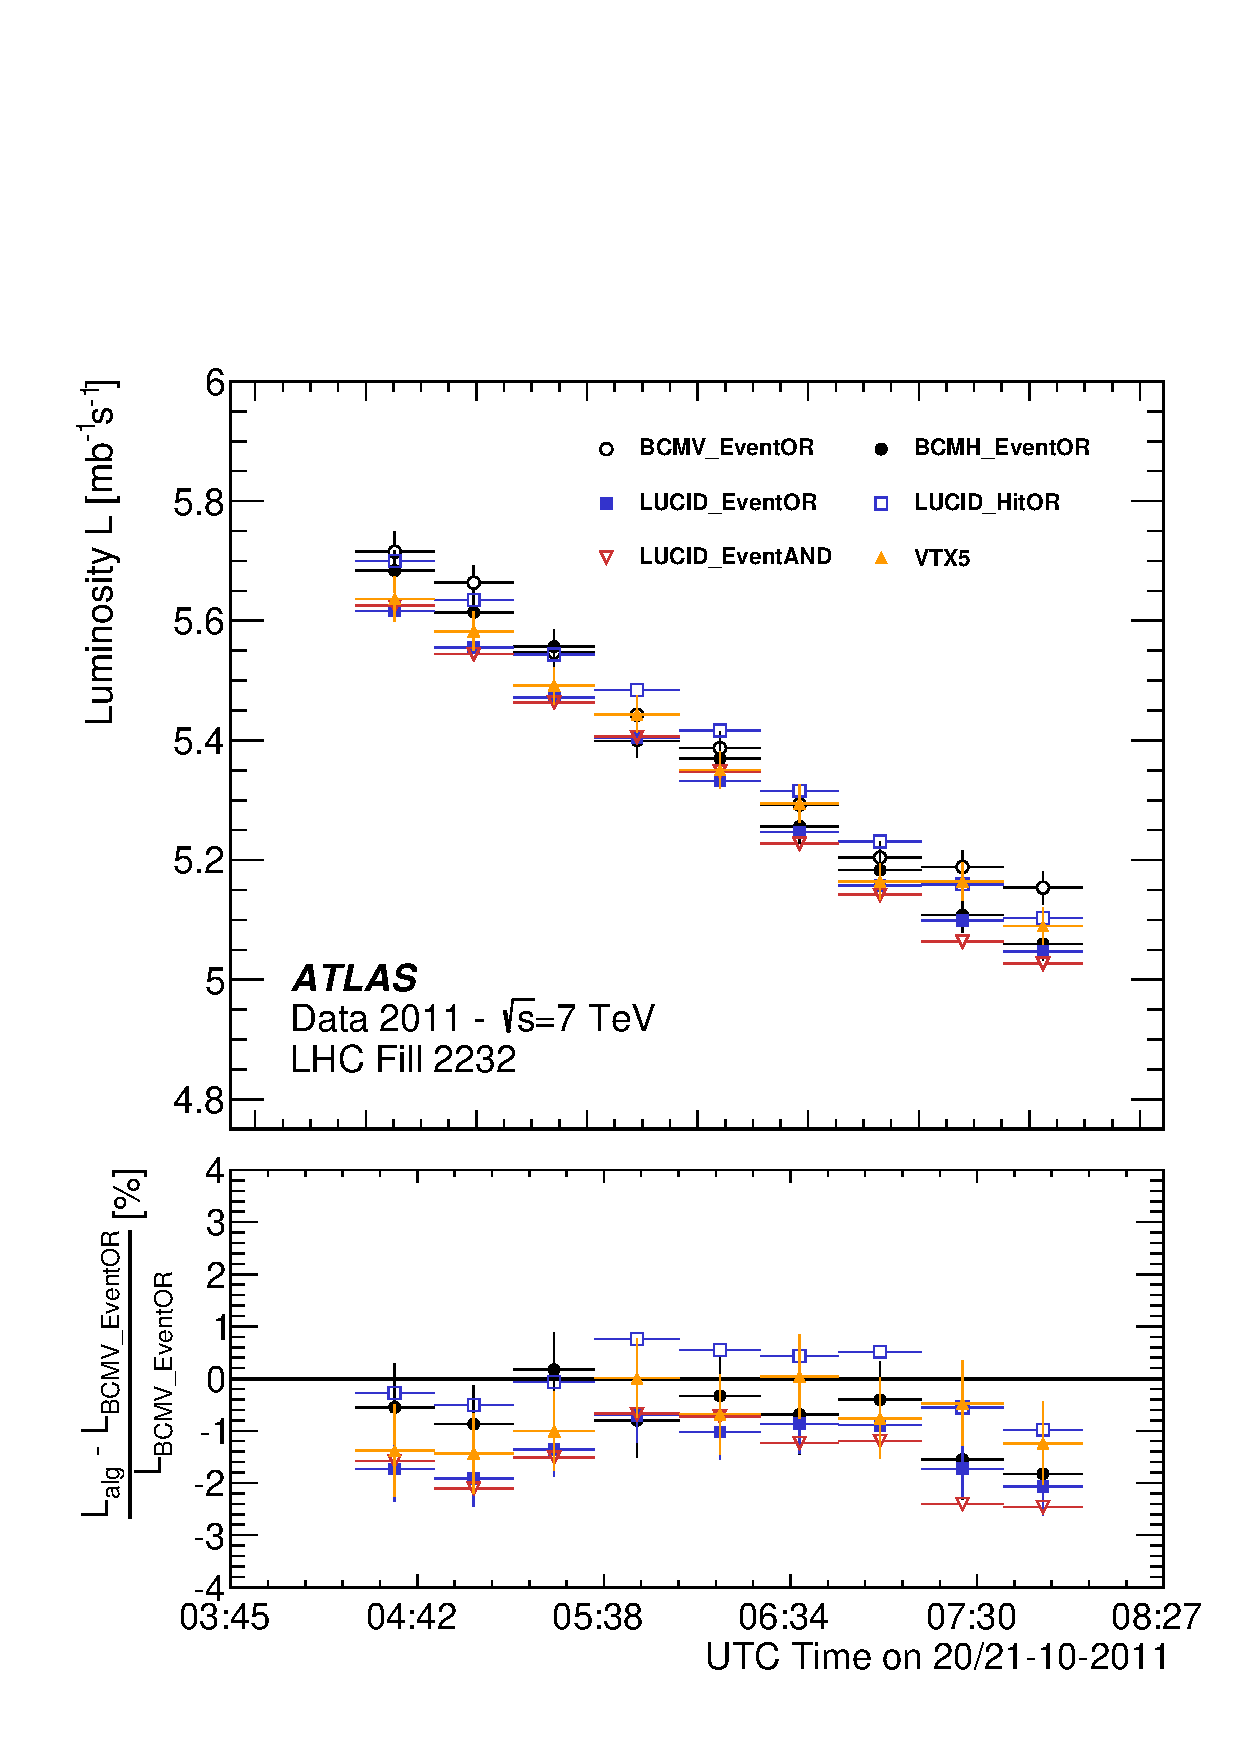
\includegraphics{figures/ch4-reconstruction/c_lumi_combined_191373.pdf}}
	\caption{Luminosities measured by BCM, LUCID, and vertex counting during the $\beta^{*}=90~\mbox{m}$ ALFA run in October 2011.}
	\label{fig:reco-luminosity-alfa}
\end{figure}

\clearpage

\section{Event Reconstruction}\label{sec:event-reconstruction}
Events are reconstructed using a wide variety of algorithms designed to identify the products of collisions at the center of the detector. The algorithms transform the raw data read out from the detector -- hits in the inner detector silicon layers and TRT straws, energy deposits in calorimeter cells, and hits in the muon stations -- into a list of physics objects and their energies or momenta. This section describes the techniques used to identify the objects used in the analyses described in chapters~\ref{ch:model-independent-trilepton-search} and \ref{ch:trilepton-resonance-search}. 


\subsection{Electrons}\label{sec:event-reconstruction-electrons}
The signature of an electron is an energy deposit in the electromagnetic LAr calorimeter and a track reconstructed by the inner detector pointing at the calorimeter energy cluster.  The electron reconstruction algorithm begins by searching for clusters of energy in the calorimeter, based on a grid of $N_{\eta}\times N_{\phi}=200\times256$ towers of size $\Delta\eta\times\Delta\phi = 0.025\times0.025$. The tower energy is the sum of the cell energies in all longitudinal layers within the tower. Energy deposits with $\Et>2.5 \GeV$ within a $3\times 5$ window of towers form the seeds for both electrons and photons.

After passing loose shower shape requirements, the electron reconstruction algorithm searches for a track within a cone of radius $\Delta R=0.3$ around the cluster barycenter. Two hypotheses are used for track pattern recognition and fitting: the standard pion hypothesis, and an electron hypothesis that allows for larger energy losses due to bremsstrahlung. The cluster and track are required to satisfy one of the following two criteria:

\begin{itemize}
	\item The barycenter of the cluster and the track extrapolation to the middle layer of the LAr calorimeter satisfy $\Delta\phi<0.2$ in the direction of track bending or $\Delta\phi<0.05$ in the other direction. 
	\item The barycenter of the cluster and the track extrapolation to the middle layer of the LAr calorimeter, after rescaling the track momentum to the energy of the cluster, satisfy $\Delta\phi<0.1$ in the direction of track bending or $\Delta\phi<0.05$ in the other direction. 
\end{itemize}
 
For tracks with at least four silicon hits, the track and the cluster must also satisfy $|\Delta\eta|<0.05$. Finally, the cluster and track are rebuilt using algorithms optimized for measurement of the electron properties. The cluster is rebuilt sequentially in all four layers, using an area of $3\times7$ layer-2 cells in the barrel or $5\times5$ layer-2 cells in the end-caps. The tracks of electron candidates are refit using an optimized electron track filter based on the Gaussian Sum Filter (GSF) algorithm~\cite{gsf}. The GSF track and the cluster must satisfy tighter spatial matching criteria: $\Delta\phi<0.1$ in the direction of track bending, or $\Delta\phi<0.05$ in the opposite direction. GSF tracks with less than four silicon hits are required to satisfy even tighter criteria: $|\Delta\eta|<0.35$ or $0.2$ in the TRT barrel or end-cap, and $\Delta\phi<0.03$ in the direction of track bending or $\Delta\phi<0.02$ in the other direction. 

\subsubsection{Identification}
Further requirements can be imposed on electron candidates to suppress backgrounds from sources like misidentified hadronic jets, photon conversions, and electrons from hadron decays. Three increasingly stringent sets of cuts are defined, called loose, medium, and tight\footnote{An alternative method of identification using a likelihood-based multivariate method has been developed, but is not used in this dissertation}. The analyses described in chapters~\ref{ch:model-independent} and \ref{ch:resonance} use the tight cuts to select signal electrons, and the medium and loose cuts to derive data-driven background estimates. The loose set of cuts impose requirements on the shower shape in the first and second calorimeter layers, the quality of the track, the fraction of energy in hadronic calorimeter cells behind the LAr cells, and the spatial match of the track and the calorimeter cluster. The medium set of cuts consist of more stringent versions of the loose cuts, and additionally require a small track impact parameter with respect to the primary vertex, a minimum number of high-threshold TRT hits associated with the track, and a hit in the innermost pixel layer. The tight set of cuts again consist of more stringent versions of the medium cuts, with an additional cut on the ratio of the cluster energy to the track momentum ($E/p$) and a veto of candidates associated to a photon conversion vertex. 

\textcolor{red}{Consider putting a table in instead of a block of text.}

\subsubsection{Efficiency Measurements}\label{sec:reco-electron-efficiency}
The efficiency to detect an electron can be factorized into several components. The efficiency to detect a cluster in the electromagnetic calorimeter is very high, above $99\%$ for electrons with $\Et=15 \GeV$ and $99.9\%$ for $\Et=45 \GeV$. The reconstruction efficiency, covering the matching of a good-quality track to the cluster, and the identification efficiencies, covering the identification cuts with respect to reconstructed electrons, are measured using tag-and-probe techniques targeting $Z\rightarrow ee$ and $J/\Psi\rightarrow ee$ events~\cite{TheATLASCollaboration:2014vz}. One electron, the tag, is required to satisfy strict selection criteria, while the second electron, the probe, is used for efficiency measurements. The combined reconstruction and identification efficiencies are shown in figure~\ref{fig:electron-id-efficiencies}. The reconstruction efficiency makes up $1-5\%$ of the efficiency loss for electrons with $\Et<20 \GeV$, and less than $1\%$ for electrons with $\Et>80 \GeV$. The efficiencies are computed for both data and simulation, and the ratio between the two is used to correct the efficiency in simulation.

\begin{figure}[htbp]
	\centering
	\subfloat[] {
		\resizebox{0.45\textwidth}{!}{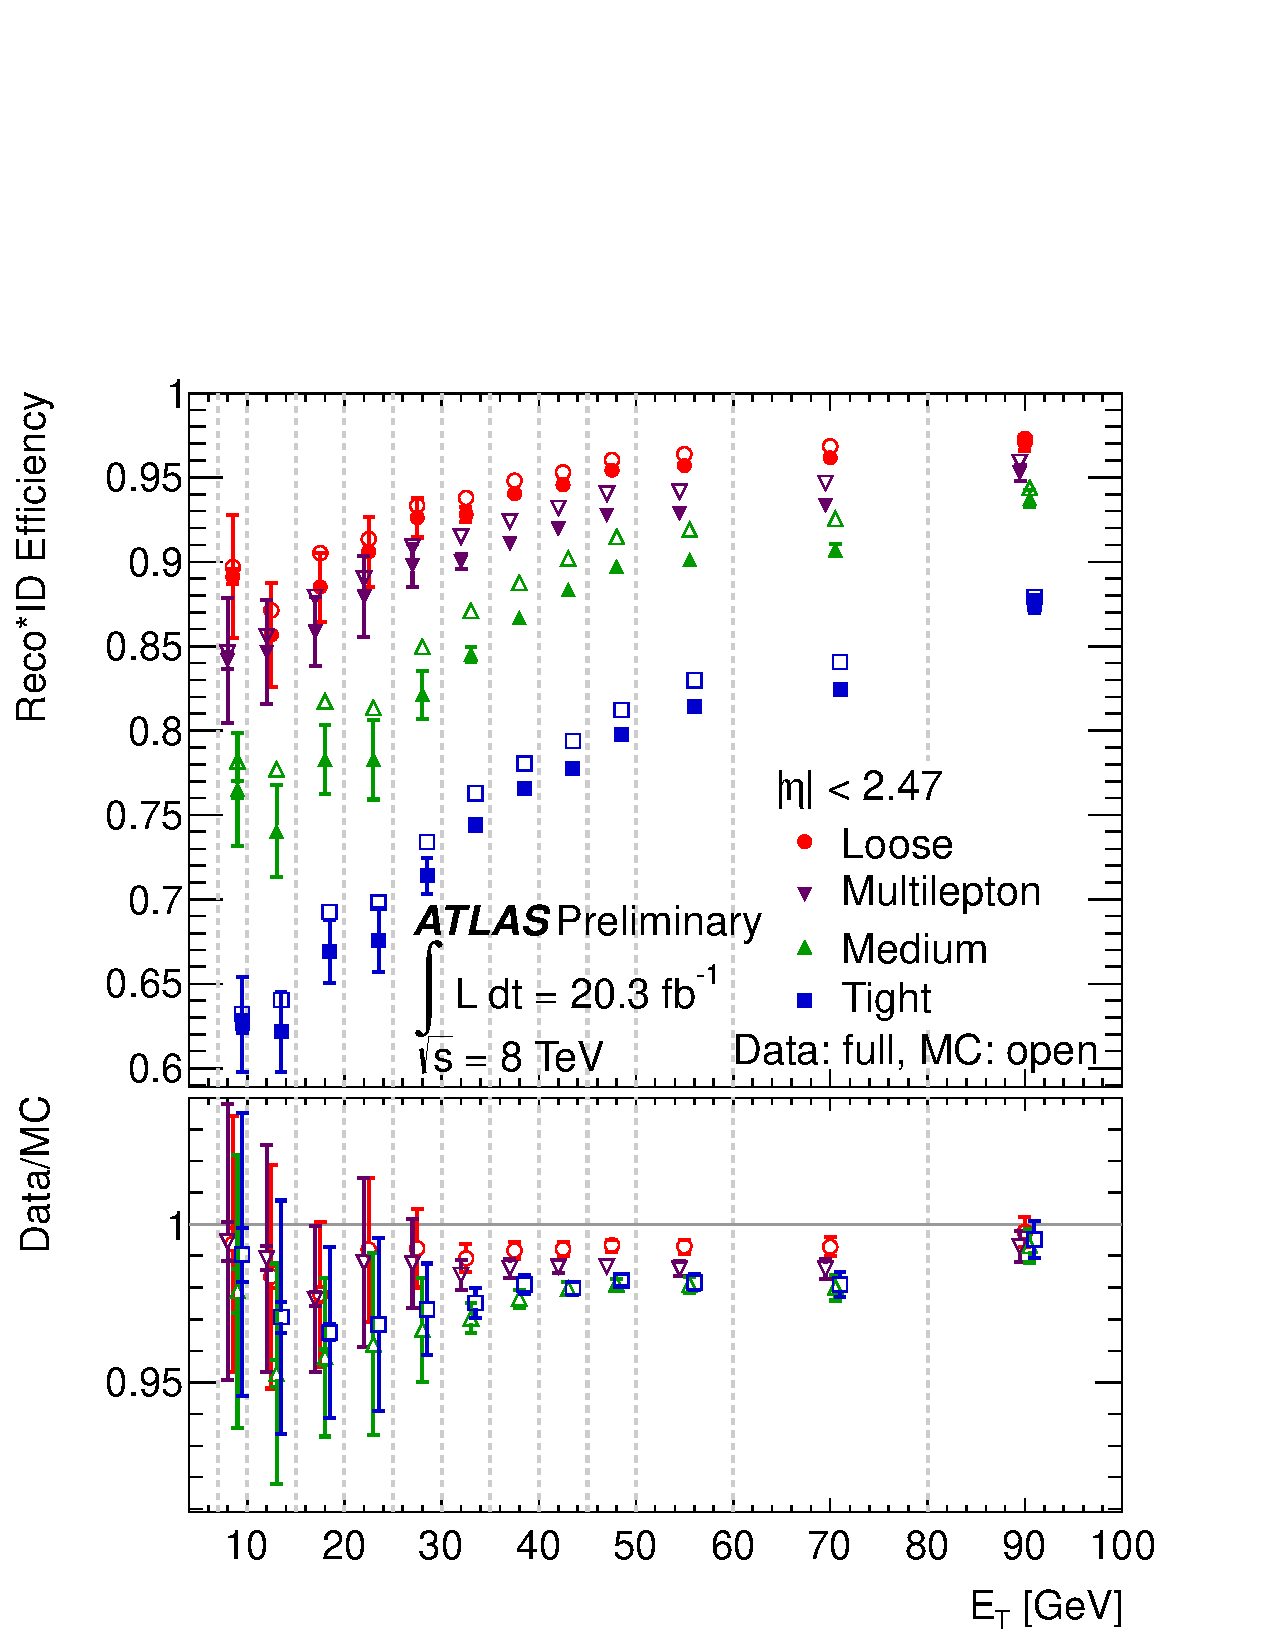
\includegraphics{figures/ch4-reconstruction/el_eff_idplusreco_ET}}
	}
	\hfill
	\subfloat[] {
		\resizebox{0.45\textwidth}{!}{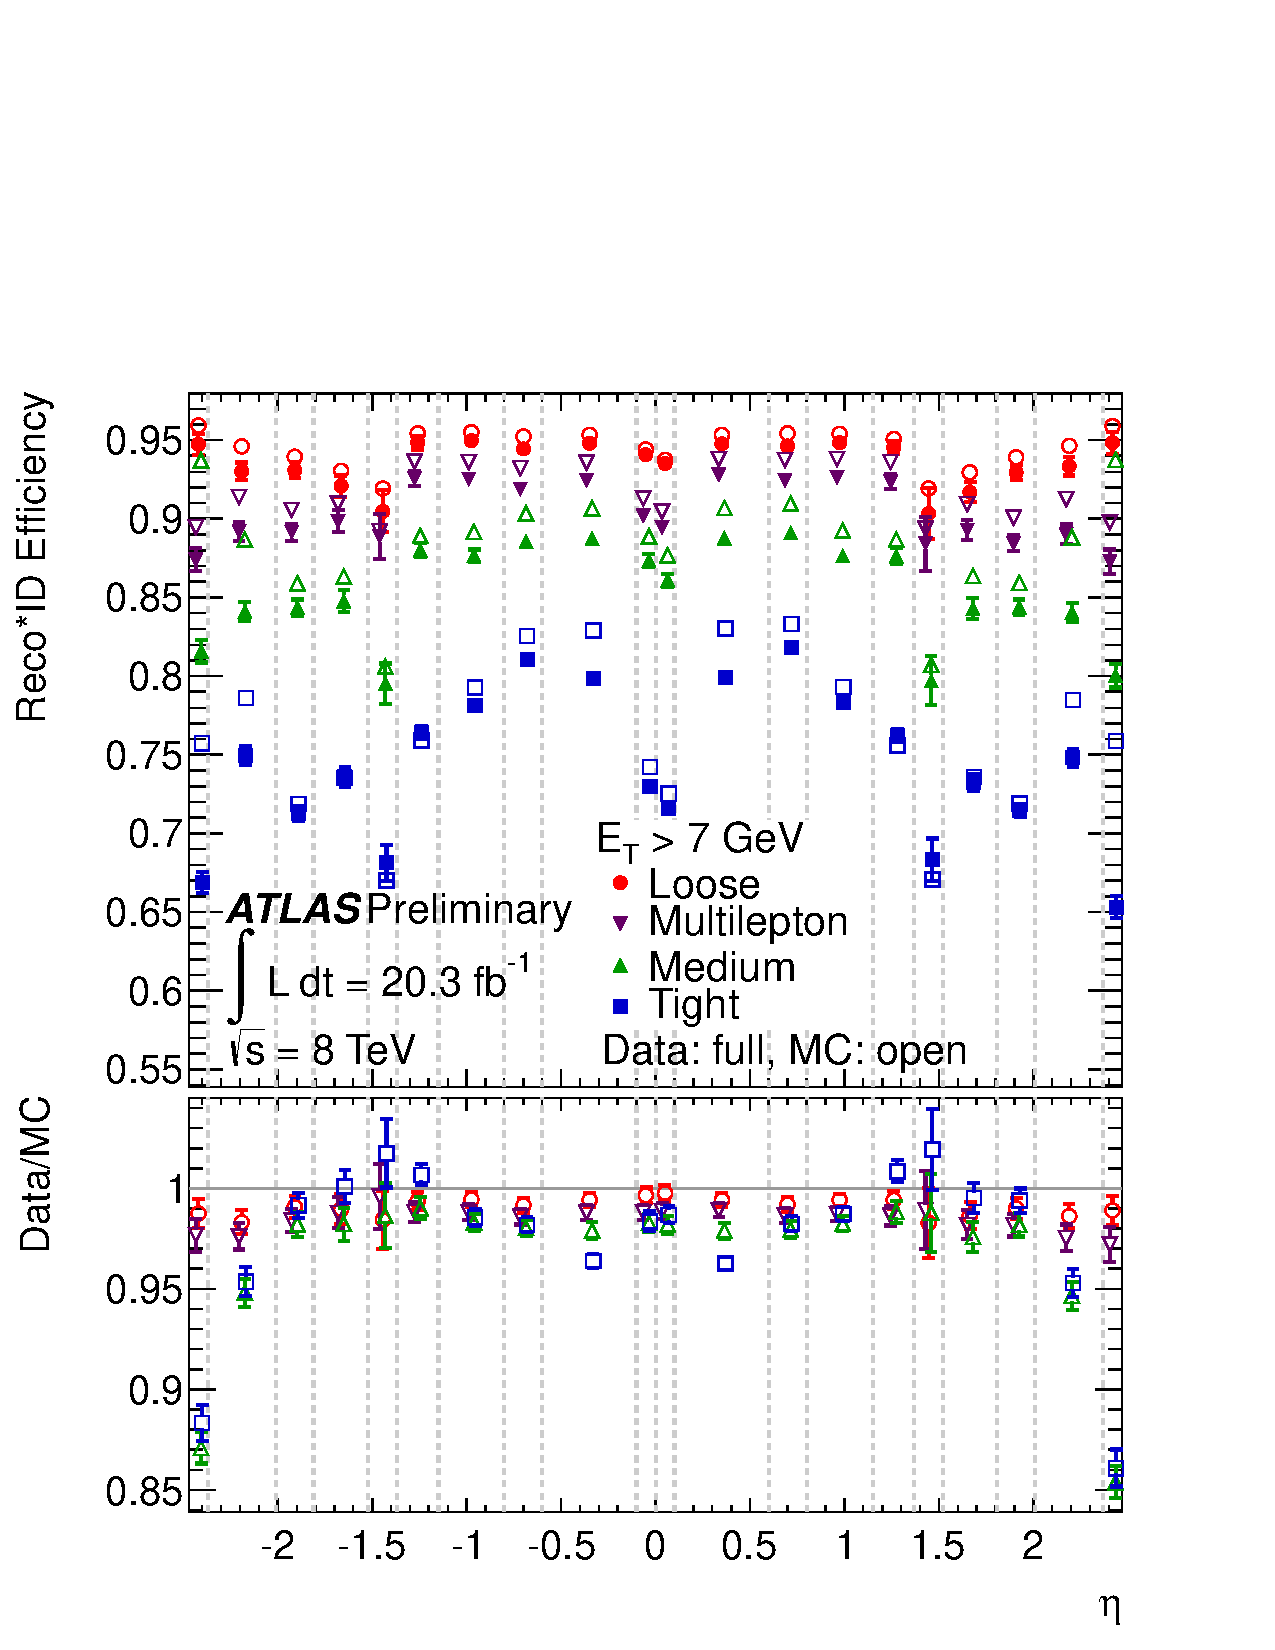
\includegraphics{figures/ch4-reconstruction/el_eff_idplusreco_eta}}
	}
	\caption{The combined reconstruction and identification efficiencies with respect to electrons detected as a cluster in the electromagnetic calorimeter, shown as a function of $\Et$ (left) and $\eta$ (right).}
	\label{fig:electron-id-efficiencies}
\end{figure}


\subsubsection{Energy and Momentum Measurement}\label{sec:reco-electron-energymomentum}
For electron candidates with at least four silicon hits, the energy of the electron is taken from the calorimeter measurement, while the trajectory is taken from the GSF track. Candidates with fewer silicon hits are not used in this dissertation. The energy resolution of the calorimeter is parametrized as:

\begin{equation}
	\frac{\sigma(E)}{E} = \frac{a}{\sqrt{e}} \oplus \frac{b}{E} \oplus c,
\end{equation}

where $a$, $b$, and $c$ are the sampling, noise, and constant terms, respectively, and generally vary with $\eta$. The design value of the sampling term is $a\approx 9-10\%$ in the central region, and worsens at higher pseudorapidities due to the increased material in front of the calorimeters. The noise term, due to electronics noise and pileup effects, is approximately $b = 350 \times \cosh\eta \MeV$. The constant term dominates the resolution at high energies, with a design value of $c=0.7\%$. 

As the ATLAS calorimeters are non-compensating, the energy measurement is calibrated using a multivariate algorithm trained on single-electron simulation to determine the most probable electron energy. The method takes into account differences between data and simulation in the energy scales of each longitudinal layer and other detector effects not modeled in simulation. 

After the initial simulation-based calibration, the electron energy scale and resolution are determined using $Z\rightarrow ee$ events. Residual differences in the energy scale between data and simulation are parametrized as:

\begin{equation}
	E^{\mathrm{data}} = E^{\mathrm{simulation}} (1 + \alpha_i),
\end{equation}

where the $\alpha_i$ quantify the energy scale difference in bins of pseudorapidity. The difference in energy resolution is derived assuming that the $Z\rightarrow ee$ invariant mass distribution is well-modeled up to a Gaussian constant term, 

\begin{equation}
	\left(\frac{\sigma_E}{E}\right)^{\mathrm{data}} = \left(\frac{\sigma_E}{E}\right)^{\mathrm{simulation}} \oplus c_i,
\end{equation}

where $i$ again denotes bins in pseudorapidity. Histograms of the $Z\rightarrow ee$ invariant mass distribution in simulation are then produced for a range of $\alpha_i$ and $c_i$ values, and the optimal values are determined using a $\chi^2$ minimization with respect to data. The results are shown in figures~\ref{fig:reco-el-EES} and \ref{fig:reco-el-EER}. 

Sources of systematic uncertainty on the energy scale include the intrinsic accuracy of the $Z\rightarrow ee$ method, determined from closure tests where known scale variations are injected into simulation, calorimeter gain and pedestal dependence, data-simulation differences in the calibration of the calorimeter layers, and the modeling of material in front of and within the calorimeter. The total uncertainty ranges from $0.03$-$0.22$\% for $\Et=40 \GeV$ and $0.27$-$2.25$\% for $\Et = 200 \GeV$, with larger uncertainties in the pseudorapidity range $1.37<|\eta|<1.82$ corresponding to the transition region between the barrel and the end-cap. 

The systematic uncertainty on the energy resolution less than $10\%$ for electrons with $\Et<50 \GeV$, and asymptotically approaches $\sim 40\%$ for high $\Et$. At low energies, the pileup contribution to the noise term, $b$, dominates the uncertainty; at higher energy, uncertainty is due to a mix of the sampling term, $a$, the pileup contribution to $b$, the modeling of material, and the intrinsic accuracy of the $Z\rightarrow ee$ method.


\subsection{Muons}\label{sec:event-reconstruction-muons}
Muons are identified by matching tracks in the muon spectrometer to tracks in the inner detector. The requirements differ based on the instrumentation available in the vicinity of the muon candidate. The analyses described here use \emph{combined} muons, consisting of tracks reconstructed independently in the inner detector and the muon spectrometer. The muon momentum is determined from a statistical combination of the two track's parameters and their corresponding covariance matrices. Combined muons have the highest purity, but suffer from a loss of acceptance near $\eta\sim 0$, where the muon spectrometer has gaps to accommodate services for the inner detector and calorimeters, and $1.1<\eta<1.3$, where some trajectories only pass through one muon station due to incomplete installation. The remaining categories are \emph{standalone} (SA) muons, consisting of a track ony in the muon spectrometer; \emph{segment-tagged} (ST) muons, consisting of an inner detector track and one or more track segments in the MDT or CSC chambers; and \emph{calorimeter-tagged} (CaloTag) muons, consisting of an inner detector track matched to a calorimeter energy deposit consistent with the passage of a muon. These categories recover efficiency in regions of the detector with less instrumentation at the cost of lower muon purity, and are not used in this dissertation. 

For all categories of muons, the inner detector track is required to have at least 1 pixel hit, at least 5 SCT hits, at most 2 pixel or SCT holes, and at least 9 TRT hits for $0.1<|\eta|<1.9$. Energy losses in the calorimeter due to ionization, bremsstrahlung, and electron pair production must also be taken into account. 

\subsubsection{Efficiency}\label{sec:reco-muon-efficiency}
The efficiency of the reconstructing CB muons is measured as:

\begin{equation}
	\epsilon(\mathrm{CB}) = \epsilon(\mathrm{CB}|\mathrm{ID}) \epsilon(\mathrm{ID}|\mathrm{MS}),
\end{equation}

where $\epsilon(\mathrm{CB}|\mathrm{ID})$ is the probability that a muon reconstructed as an inner detector track is also reconstructed as a CB muon, and $\epsilon(\mathrm{ID}|\mathrm{MS})\approx \epsilon(\mathrm{ID})$ is the probability that a muon with a track in the muon spectrometer, i.e. a CB or SA muon, is also reconstructed as an inner detector track. The latter approximation is made because $\epsilon(\mathrm{ID})$ is not directly accessible in data. 

The efficiencies are measured using tag-and-probe techniques similar to those described in section~\ref{sec:reco-electron-efficiency}, targeting $Z\rightarrow\mu\mu$ and $J/\Psi\rightarrow\mu\mu$ events. In this case, the tag muon is required to be a CB muon, and the probe muon is a CB or SA muon in the case of measuring $\epsilon(\mathrm{ID}|\mathrm{MS})$, and a CaloTag muon for the measurement of $\epsilon(\mathrm{CB}|\mathrm{ID})$. The efficiencies for all types of muon are shown in figure~\ref{fig:reco-muon-efficiency}. CB muons have an efficiency of greater than $97\%$ in most of the pseudorapidity range, except for significant inefficiencies due to gaps in the muon spectrometer in the ranges $|\eta|<0.1$ and $1.1<\eta<1.3$. The measured efficiencies in data and simulation agree to within $\sim2\%$, and the ratios in each pseudorapidity bin are used as scale factors to correct the efficiency in simulation. The systematic uncertainty on the scale factors is in the range $0.1$-$0.3\%$, rising near $|\eta|\sim 0$ and $|\eta|\sim 2.5$.

\begin{figure}[htbp]
	\centering
	Figure 3 from muon paper, and 5a
	\caption{Top: Muon reconstruction efficiencies as a function of $\eta$ for muons with $\pt>10 \GeV$. The uncertainty bars on the points indicate statistical uncertainties. Bottom: The ratio between the measured and simulated efficiencies, with the combination of statistical and systematic uncertainties indicated by the uncertainty bars.}
	\label{fig:reco-muon-efficiency}
\end{figure}


\subsubsection{Energy Scale and Resolution}
The muon momenta in simulation are scaled and smeared to match the momentum scale and resolution in data. The corrections are derived in bins of $\eta$ and $\phi$, with boundaries chosen to minimize the variation of the correction in each bin, and are applied separately to the transverse momenta measured by the inner detector (ID) and the muon spectrometer (MS). Specifically, the correction is implemented as:

\begin{equation}
	\pt^{\mathrm{Cor,Det}} = \frac{\pt^{\mathrm{MC,Det}} + \sum_{n=0}^1 s_n^{\mathrm{Det}(\eta,\phi)(\pt^{\mathrm{MC,Det}})^n}}{1+\sum_{m=0}^2 \Delta r_m^{\mathrm{Det}}(\eta,\phi)(\pt^{\mathrm{MC,Det}})^{m-1}g_m},
\end{equation}

where Det=ID or MS, the $\Delta r_m^{\mathrm{Det}}(\eta,\phi)$ parametrize the momentum resolution smearing, the $s_n^{\mathrm{Det}}(\eta,\phi)$ parametrize the scale corrections, and the $g_m$ are normally-distributed random variable with mean 0 and width 1\footnote{Note that this equation does not apply to cases where the resolution is data is better than that in simulation. In these cases, the resolution difference is included in the positive ID and MS variations, and the effect of the positive variation on the physical observables is symmetrized about the nominal value.}. The constant scale correction term, $s_0^{\mathrm{MS}}$, accounts for the difference between data and simulation in the energy lost by muons before reaching the muon spectrometer. $s_0^{\mathrm{ID}}$ is set to zero due to the negligible energy loss before the inner detector. The linear terms, $s_1^{\mathrm{ID,MS}}$, models discrepancies between data and simulation in the magnetic field integral and the radial dimension of the detector. The resolution corrections $\Delta r_m^{\mathrm{Det}}$ represent deviations from the resolution in data, which is parametrized empirically as:

\begin{equation}
	\frac{\sigma(\pt)}{\pt} = \frac{r_0}{\pt} \oplus r_1 \oplus r2\cdot\pt,
\end{equation}

where the $r_0$ term describes energy lost by muons as they traverse the material of the detector, the $r_1$ term describes multiple scattering, magnetic field inhomogeneities, and local radial displacements, and the $r_2$ term describes intrinsic resolution effects due to the spatial resolution of the hit measurements and residual misalignment. 

The corrections are derived from $J/\Psi\rightarrow\mu\mu$, $\Upsilon\rightarrow\mu\mu$, and $Z\rightarrow\mu\mu$ events using a template maximum likelihood fit, similar to that described in section~\ref{sec:reco-electron-energymomentum}. The effect of the corrections on the invariant mass distribution of $Z\rightarrow\mu\mu$ events is shown in figure~\ref{fig:reco-muon-momentum-corrections}, along with the total systematic uncertainty. \textcolor{red}{Consider showing the muon momentum resolution, figure 14.}

\begin{figure}
	Figure 10c
	\label{fig:reco-muon-momentum-corrections}
\end{figure}



\subsection{Tau Leptons}\label{sec:event-reconstruction-taus}
The signature of tau leptons is significantly more complex than electrons and muons due to the fact that they decay to a diverse set of final states. Tau leptons have a proper decay length of $87 \um$, and therefore typically decay before reaching the active layers of the detector. The leading decay modes are shown in table~\ref{table:reco-tau-decays}. $35.2\%$ of tau leptons decay to an electron or muon plus two neutrinos. The remaining $64.8\%$ decay to hadrons plus a neutrino. The hadronic decay modes contain one charged pion in $72\%$ of the decays, and three charged pions in $22\%$ of the decays; the majority of the remainder contain one or more charged kaons. The hadronic decay modes also frequently contain neutral pions, with $78\%$ containing at least one neutral pion. 



\subsubsection{Efficiency}

\subsubsection{Energy Scale and Resolution}



\subsection{Jets}\label{sec:event-reconstruction-jets}

%\subsubsection{Efficiency}

\subsubsection{Energy Scale and Resolution}

\subsubsection{$B$-tagging}\label{sec:event-reconstruction-bjets}

\subsection{Invisible Particles}\label{sec:event-reconstruction-met}
